% !TeX program = lualatex
% ALIUS Bulletin native visual reconstruction source.
% Generated from off-repo reference layout data; does not include or input a pre-existing article PDF.
\ifdefined\ALIUSIssueBuild
\else
\documentclass{article}
\usepackage[paperwidth=595.0000bp,paperheight=842.0000bp,margin=0bp]{geometry}
\usepackage{graphicx}
\usepackage{xcolor}
\usepackage{tikz}
\usepackage{iftex}
\usepackage[hidelinks]{hyperref}
\ifPDFTeX
  \usepackage[T1]{fontenc}
  \usepackage[utf8]{inputenc}
  \usepackage{textcomp}
  \usepackage{amssymb}
\else
  \usepackage{fontspec}
\fi
\pagestyle{empty}
\fi
\ifPDFTeX
  \providecommand{\ALIUSDeclareUnicodeFallbacks}{%
    \DeclareUnicodeCharacter{00AC}{\ensuremath{\neg}}%
    \DeclareUnicodeCharacter{00BE}{\ensuremath{\frac{3}{4}}}%
    \DeclareUnicodeCharacter{0101}{\=a}%
    \DeclareUnicodeCharacter{0107}{\'c}%
    \DeclareUnicodeCharacter{012B}{\=\i}%
    \DeclareUnicodeCharacter{0131}{\i}%
    \DeclareUnicodeCharacter{0142}{\l}%
    \DeclareUnicodeCharacter{015B}{\'s}%
    \DeclareUnicodeCharacter{016B}{\=u}%
    \DeclareUnicodeCharacter{025C}{q}%
    \DeclareUnicodeCharacter{0278}{t}%
    \DeclareUnicodeCharacter{02AE}{Th}%
    \DeclareUnicodeCharacter{02B0}{ff}%
    \DeclareUnicodeCharacter{02B4}{ffi}%
    \DeclareUnicodeCharacter{02BE}{ft}%
    \DeclareUnicodeCharacter{02BF}{fi}%
    \DeclareUnicodeCharacter{02C0}{fl}%
    \DeclareUnicodeCharacter{02C1}{fi}%
    \DeclareUnicodeCharacter{02D9}{Th}%
    \DeclareUnicodeCharacter{02EF}{gy}%
    \DeclareUnicodeCharacter{0394}{\ensuremath{\Delta}}%
    \DeclareUnicodeCharacter{03B2}{\ensuremath{\beta}}%
    \DeclareUnicodeCharacter{03BA}{\ensuremath{\kappa}}%
    \DeclareUnicodeCharacter{068D}{-}%
    \DeclareUnicodeCharacter{08BC}{ti}%
    \DeclareUnicodeCharacter{099E}{ti}%
    \DeclareUnicodeCharacter{1E43}{\d{m}}%
    \DeclareUnicodeCharacter{1E47}{\d{n}}%
    \DeclareUnicodeCharacter{1E63}{\d{s}}%
    \DeclareUnicodeCharacter{201C}{``}%
    \DeclareUnicodeCharacter{201D}{''}%
    \DeclareUnicodeCharacter{2260}{\ensuremath{\neq}}%
    \DeclareUnicodeCharacter{25A1}{\ensuremath{\square}}%
  }%
  \ifdefined\ALIUSIssueBuild\else\ALIUSDeclareUnicodeFallbacks\fi
  \providecommand{\ALIUSFontLatoLight}{\fontfamily{lato-LF}\fontseries{l}\selectfont}
  \providecommand{\ALIUSFontLatoRegular}{\fontfamily{lato-LF}\fontseries{m}\selectfont}
  \providecommand{\ALIUSFontLatoItalic}{\fontfamily{lato-LF}\fontseries{m}\itshape}
  \providecommand{\ALIUSFontLatoLightItalic}{\fontfamily{lato-LF}\fontseries{l}\itshape}
  \providecommand{\ALIUSFontCormorantRegular}{\fontfamily{CormorantGaramond-LF}\fontseries{m}\selectfont}
  \providecommand{\ALIUSFontCormorantLight}{\fontfamily{CormorantGaramond-LF}\fontseries{l}\selectfont}
  \providecommand{\ALIUSFontCormorantMedium}{\fontfamily{CormorantGaramond-LF}\fontseries{medium}\selectfont}
  \providecommand{\ALIUSFontCormorantBold}{\fontfamily{CormorantGaramond-LF}\fontseries{b}\selectfont}
  \providecommand{\ALIUSFontCormorantItalic}{\fontfamily{CormorantGaramond-LF}\fontseries{m}\itshape}
  \providecommand{\ALIUSFontTimes}{\fontfamily{ptm}\selectfont}
  \providecommand{\ALIUSFontCalibri}{\fontfamily{phv}\selectfont}
  \providecommand{\ALIUSFontCambria}{\fontfamily{ptm}\selectfont}
  \providecommand{\ALIUSFontSymbolFallback}{\fontfamily{ptm}\selectfont}
\else
  \providecommand{\ALIUSFontLatoLight}{\fontspec{Lato Light}}
  \providecommand{\ALIUSFontLatoRegular}{\fontspec{Lato Regular}}
  \providecommand{\ALIUSFontLatoItalic}{\fontspec{Lato Italic}}
  \providecommand{\ALIUSFontLatoLightItalic}{\fontspec{Lato Light Italic}}
  \providecommand{\ALIUSFontCormorantRegular}{\fontspec{Cormorant Garamond Regular}}
  \providecommand{\ALIUSFontCormorantLight}{\fontspec{Cormorant Garamond Light}}
  \providecommand{\ALIUSFontCormorantMedium}{\fontspec{Cormorant Garamond Medium}}
  \providecommand{\ALIUSFontCormorantBold}{\fontspec{Cormorant Garamond Bold}}
  \providecommand{\ALIUSFontCormorantItalic}{\fontspec{Cormorant Garamond Italic}}
  \providecommand{\ALIUSFontTimes}{\fontspec{Times New Roman}}
  \providecommand{\ALIUSFontCalibri}{\fontspec{Calibri}}
  \providecommand{\ALIUSFontCambria}{\fontspec{Cambria}}
  \providecommand{\ALIUSFontSymbolFallback}{\fontspec{Times New Roman}}
\fi
\providecommand{\ALIUSPullQuoteOpen}{\textquotedblleft}
\providecommand{\ALIUSPullQuoteClose}{\textquotedblright}
\providecommand{\ALIUSPullQuoteBlockAt}[4]{%
  \node[anchor=north west,inner sep=0pt,outer sep=0pt,text=ALIUSC7F7F7F] at (#1bp,-#2bp) {%
    {\ALIUSFontCormorantLight\fontsize{32.000bp}{32.000bp}\selectfont\ALIUSPullQuoteOpen}%
  };%
  \node[anchor=north west,inner sep=0pt,outer sep=0pt,xshift=24bp,text width=\dimexpr#3bp-48bp\relax,align=center,text=ALIUSC595959,font=\ALIUSFontLatoLight\fontsize{15.000bp}{18.000bp}\selectfont] (ALIUSPullQuoteBody) at (#1bp,-#2bp) {#4};%
  \node[anchor=south east,inner sep=0pt,outer sep=0pt,text=ALIUSC7F7F7F,xshift=24bp] at (ALIUSPullQuoteBody.south east) {%
    {\ALIUSFontCormorantLight\fontsize{32.000bp}{32.000bp}\selectfont\ALIUSPullQuoteClose}%
  };%
}
\providecommand{\ALIUSNotableQuoteAt}[4]{%
  \ALIUSPullQuoteBlockAt{#1}{#2}{#3}{#4}%
}
\providecommand{\ALIUSMaybeNotableQuoteAt}[4]{%
  \if\relax\detokenize{#4}\relax\else\ALIUSNotableQuoteAt{#1}{#2}{#3}{#4}\fi%
}
\providecommand{\ALIUSRefAnchor}[1]{\hypertarget{#1}{}}
\providecommand{\ALIUSCitationLink}[2]{\hyperlink{#1}{#2}}
\definecolor{ALIUSC000000}{HTML}{000000}
\definecolor{ALIUSC0563C1}{HTML}{0563C1}
\definecolor{ALIUSC1A1718}{HTML}{1A1718}
\definecolor{ALIUSC1F8135}{HTML}{1F8135}
\definecolor{ALIUSC595959}{HTML}{595959}
\definecolor{ALIUSC767171}{HTML}{767171}
\definecolor{ALIUSC7F7F7F}{HTML}{7F7F7F}
\definecolor{ALIUSCBFBFBF}{HTML}{BFBFBF}
\providecommand{\ALIUSPlacedText}[6]{%
  \node[anchor=north west,inner sep=0pt,outer sep=0pt,text=#4] at (#1bp,-#2bp) {%
    \resizebox{#3bp}{!}{{#5\fontsize{#6bp}{#6bp}\selectfont #6\kern0pt}}%
  };%
}
\providecommand{\ALIUSPlacedTextContent}[7]{%
  \node[anchor=north west,inner sep=0pt,outer sep=0pt,text=#4] at (#1bp,-#2bp) {%
    \resizebox{#3bp}{!}{{#5\fontsize{#6bp}{#6bp}\selectfont #7}}%
  };%
}
% --- Draft abstract retained as comments; not rendered in reconstruction. ---
% \section*{Abstract}
% This interview with Karl Friston presents a Bayesian account of cognition, life, and consciousness centred on the free energy principle. Friston recounts the origin of the principle in a childhood "Gerald Durrell" moment observing woodlice in the sun, later crystallized through Arthur Eddington's writings on space-time and developed mathematically through variational Bayes and ensemble density dynamics. He clarifies the relations among the Bayesian brain hypothesis, predictive coding, and the free energy principle by distinguishing principle from process theory, casting predictive coding as one of many ways to minimize variational free energy, and emphasizing the enactive, embodied, extended, embedded, and encultured aspect captured by active inference. The conversation maps these frameworks onto David Marr's three levels of analysis and proposes a six-level hierarchy of mind and brain running from peripheral reflexes through percepts, concepts, and narratives to self-awareness, with Markov blankets separating levels in ways consistent with Thomas Metzinger's self-modeling. Friston defends the view that all interesting states are low-entropy, recasting altered states through the resolution of uncertainty and the epistemic affordance of exploration. Further sections take up precision as the determinant of whether prediction errors are expressed phenomenologically, the "representation wars" between embodied and representationalist readings of the framework, and computational psychiatry, where Friston argues that process-based and precision-based models of psychosis collapse into a single story of false inference grounded in aberrant precision encoding. The interview closes on consciousness as a process of inference and self-evidencing, with self-awareness requiring counterfactual breadth and a generative model distinguishing self from other.\par
% --- End draft abstract. ---
\ifdefined\ALIUSIssueBuild
\else
\begin{document}
\fi
% Page 1
\thispagestyle{empty}
\noindent\begin{tikzpicture}[remember picture,overlay,x=1bp,y=1bp,shift={(current page.north west)}]
  \fill[ALIUSC767171] (69.640bp,-787.000bp) rectangle ++(456.480bp,-0.720bp);
  \fill[ALIUSC1F8135] (352.840bp,-161.320bp) rectangle ++(71.520bp,-0.240bp);
  \fill[ALIUSC1F8135] (352.840bp,-217.720bp) rectangle ++(80.880bp,-0.240bp);
  \fill[ALIUSC1F8135] (352.840bp,-277.720bp) rectangle ++(69.600bp,-0.240bp);
  \fill[ALIUSCBFBFBF] (347.320bp,-132.520bp) rectangle ++(0.240bp,-122.640bp);
  \fill[ALIUSCBFBFBF] (347.320bp,-255.160bp) rectangle ++(0.240bp,-2.160bp);
  \fill[ALIUSCBFBFBF] (347.320bp,-257.320bp) rectangle ++(0.240bp,-48.000bp);
  \ALIUSPlacedTextContent{511.620}{35.460}{14.844}{ALIUSC767171}{\ALIUSFontLatoLight}{10.800}{17}
  \ALIUSPlacedTextContent{71.080}{71.099}{191.242}{ALIUSC000000}{\ALIUSFontLatoRegular}{19.920}{Of woodlice and men}
  \ALIUSPlacedTextContent{71.080}{95.311}{420.572}{ALIUSC000000}{\ALIUSFontLatoLight}{17.755}{A Bayesian account of cognition, life and consciousness}
  \ALIUSPlacedTextContent{69.400}{132.486}{125.486}{ALIUSC000000}{\ALIUSFontLatoLight}{15.840}{An interview with}
  \ALIUSPlacedTextContent{352.840}{137.940}{59.107}{ALIUSC000000}{\ALIUSFontLatoRegular}{10.800}{Karl Friston}
  \ALIUSPlacedTextContent{352.840}{151.355}{73.163}{ALIUSC1F8135}{\ALIUSFontLatoLight}{8.880}{k.friston@ucl.ac.uk}
  \ALIUSPlacedTextContent{69.400}{151.726}{99.589}{ALIUSC000000}{\ALIUSFontLatoLight}{18.960}{Karl Friston}
  \ALIUSPlacedTextContent{352.840}{162.155}{168.215}{ALIUSC000000}{\ALIUSFontLatoLight}{8.880}{Wellcome Centre for Human Neuroimaging}
  \ALIUSPlacedTextContent{352.840}{172.955}{120.947}{ALIUSC000000}{\ALIUSFontLatoLight}{8.880}{University College London, UK}
  \ALIUSPlacedTextContent{69.400}{186.448}{218.543}{ALIUSC000000}{\ALIUSFontLatoLight}{12.960}{By Martin Fortier \& Daniel A. Friedman}
  \ALIUSPlacedTextContent{352.840}{194.340}{71.262}{ALIUSC000000}{\ALIUSFontLatoRegular}{10.800}{Martin Fortier}
  \ALIUSPlacedTextContent{352.840}{207.755}{82.654}{ALIUSC1F8135}{\ALIUSFontLatoLight}{8.880}{martin.fortier@ens.fr}
  \ALIUSPlacedTextContent{352.840}{218.555}{74.000}{ALIUSC000000}{\ALIUSFontLatoLight}{8.880}{Institut Jean Nicod}
  \ALIUSPlacedTextContent{352.840}{229.355}{101.584}{ALIUSC000000}{\ALIUSFontLatoLight}{8.880}{ENS/EHESS, Paris, France}
  \ALIUSPlacedTextContent{352.840}{254.340}{91.431}{ALIUSC000000}{\ALIUSFontLatoRegular}{10.800}{Daniel A. Friedman}
  % ALIUS normalized citation panel begin
  % ALIUS normalized citation panel text: Cite as: Friston, K., Fortier, M. \& Friedman, D. A. (2018). Of woodlice and men: A Bayesian account of cognition, life and consciousness. An interview with Karl Friston. ALIUS Bulletin 17-43.
  \fill[white] (67.900bp,-255.448bp) rectangle ++(252.991bp,-51.300bp);
  \node[anchor=north west,inner sep=0pt,outer sep=0pt,text=ALIUSC000000] at (69.400bp,-257.448bp) {\begin{minipage}{249.991bp}{\ALIUSFontLatoLight\fontsize{9.200bp}{10.700bp}\selectfont\raggedright Cite as: Friston, K., Fortier, M. \& Friedman, D. A. (2018). Of woodlice and men: A Bayesian account of cognition, life and consciousness. An interview with Karl Friston. ALIUS Bulletin 17-43. \mbox{\textcolor{ALIUSC1F8135}{\href{https://doi.org/10.34700/h460-nz89}{https://doi.org/10.34700/h460-nz89}}}\par}\end{minipage}};
  % ALIUS normalized citation panel end
  \ALIUSPlacedTextContent{352.840}{267.755}{71.368}{ALIUSC1F8135}{\ALIUSFontLatoLight}{8.880}{dfri@stanford.edu}
  \ALIUSPlacedTextContent{352.840}{278.555}{88.908}{ALIUSC000000}{\ALIUSFontLatoLight}{8.880}{Department of Biology}
  \ALIUSPlacedTextContent{329.391}{281.448}{14.558}{ALIUSC000000}{\ALIUSFontLatoLight}{9.840}{, 2,}
  \ALIUSPlacedTextContent{352.840}{289.355}{97.242}{ALIUSC000000}{\ALIUSFontLatoLight}{8.880}{Stanford University, USA}
  \ALIUSPlacedTextContent{71.080}{353.728}{453.293}{ALIUSC1F8135}{\ALIUSFontLatoLight}{12.960}{You are well known for being the founder of the free energy principle, a wide-}
  \ALIUSPlacedTextContent{71.080}{369.328}{455.868}{ALIUSC1F8135}{\ALIUSFontLatoLight}{12.960}{ranging theoretical framework aiming to unify the psychological, neural and}
  \ALIUSPlacedTextContent{71.080}{384.928}{455.754}{ALIUSC1F8135}{\ALIUSFontLatoLight}{12.960}{biological nature of living beings (\ALIUSCitationLink{aliusref-friston-fortier-friedman-friston-2010}{Friston, 2010}, 2013; Ramstead, Badcock, \&}
  \ALIUSPlacedTextContent{71.080}{400.528}{455.706}{ALIUSC1F8135}{\ALIUSFontLatoLight}{12.960}{Friston, 2017). When did you first come up with the idea of the free energy}
  \ALIUSPlacedTextContent{71.080}{416.128}{455.912}{ALIUSC1F8135}{\ALIUSFontLatoLight}{12.960}{principle? How did this first insight gradually develop to the point of being such a}
  \ALIUSPlacedTextContent{71.080}{431.728}{158.869}{ALIUSC1F8135}{\ALIUSFontLatoLight}{12.960}{groundbreaking framework?}
  \ALIUSPlacedTextContent{71.080}{459.258}{456.544}{ALIUSC1A1718}{\ALIUSFontCormorantRegular}{13.920}{I first came up with a prototypical free energy principle when I was eight years old,}
  \ALIUSPlacedTextContent{71.080}{476.058}{456.566}{ALIUSC1A1718}{\ALIUSFontCormorantRegular}{13.920}{in what I have previously called a "Gerald Durrell" moment (\ALIUSCitationLink{aliusref-friston-fortier-friedman-friston-2012}{Friston, 2012}). I was in}
  \ALIUSPlacedTextContent{71.080}{493.098}{456.662}{ALIUSC1A1718}{\ALIUSFontCormorantRegular}{13.920}{the garden, during a gloriously hot 1960s British summer, preoccupied with the}
  \ALIUSPlacedTextContent{71.080}{510.138}{298.931}{ALIUSC1A1718}{\ALIUSFontCormorantRegular}{13.920}{antics of some woodlice (small armadillo like bugs—see}
  \ALIUSPlacedTextContent{369.296}{510.138}{38.191}{ALIUSC1A1718}{\ALIUSFontCormorantItalic}{13.920}{Figure 1}
  \ALIUSPlacedTextContent{407.510}{510.138}{120.138}{ALIUSC1A1718}{\ALIUSFontCormorantRegular}{13.920}{) who were frantically}
  \ALIUSPlacedTextContent{71.080}{526.938}{241.113}{ALIUSC1A1718}{\ALIUSFontCormorantRegular}{13.920}{scurrying around trying to find some shade.}
  \ALIUSPlacedTextContent{71.080}{555.978}{456.592}{ALIUSC1A1718}{\ALIUSFontCormorantRegular}{13.920}{After half an hour of observation and innocent (childlike) contemplation, I realized}
  \ALIUSPlacedTextContent{71.080}{573.018}{456.686}{ALIUSC1A1718}{\ALIUSFontCormorantRegular}{13.920}{their "scurrying" had no purpose or intent: they were simply moving faster in the}
  \ALIUSPlacedTextContent{71.080}{589.818}{456.529}{ALIUSC1A1718}{\ALIUSFontCormorantRegular}{13.920}{sun—and slower in the shade. The simplicity of this explanation—for what one could}
  \ALIUSPlacedTextContent{71.080}{606.858}{65.357}{ALIUSC1A1718}{\ALIUSFontCormorantRegular}{13.920}{artfully call}
  \ALIUSPlacedTextContent{136.229}{606.858}{113.133}{ALIUSC1A1718}{\ALIUSFontCormorantItalic}{13.920}{biotic self-organization}
  \ALIUSPlacedTextContent{249.399}{606.858}{278.288}{ALIUSC1A1718}{\ALIUSFontCormorantRegular}{13.920}{—appealed to me then and appeals to me now. It is}
  \ALIUSPlacedTextContent{71.080}{623.658}{456.687}{ALIUSC1A1718}{\ALIUSFontCormorantRegular}{13.920}{exactly the same principle that underwrites the ensemble density dynamics of the}
  \ALIUSPlacedTextContent{71.080}{640.698}{246.881}{ALIUSC1A1718}{\ALIUSFontCormorantRegular}{13.920}{free energy principle—and all its corollaries.}
  \ALIUSPlacedTextContent{71.080}{669.738}{453.234}{ALIUSC1A1718}{\ALIUSFontCormorantRegular}{13.920}{The beautiful simplicity (or nihilistic tautology) of this sort of explanation for life—}
  \ALIUSPlacedTextContent{71.080}{686.538}{252.921}{ALIUSC1A1718}{\ALIUSFontCormorantRegular}{13.920}{and creatures like us—crystallized in my teens}
  \ALIUSPlacedTextContent{323.888}{686.538}{203.783}{ALIUSC000000}{\ALIUSFontCormorantRegular}{13.920}{(for an autobiographical account, see}
  \ALIUSPlacedTextContent{71.080}{703.578}{271.290}{ALIUSC000000}{\ALIUSFontCormorantRegular}{13.920}{my personal supplementary material in this issue)}
  \ALIUSPlacedTextContent{342.448}{703.578}{185.238}{ALIUSC1A1718}{\ALIUSFontCormorantRegular}{13.920}{. My father thought it would be a}
  \ALIUSPlacedTextContent{71.080}{720.618}{149.771}{ALIUSC1A1718}{\ALIUSFontCormorantRegular}{13.920}{good idea for me to read}
  \ALIUSPlacedTextContent{223.443}{720.618}{151.987}{ALIUSC1A1718}{\ALIUSFontCormorantItalic}{13.920}{Space, Time and Gravitation}
  \ALIUSPlacedTextContent{375.439}{720.618}{152.198}{ALIUSC1A1718}{\ALIUSFontCormorantRegular}{13.920}{by Sir Arthur Eddington}
  \ALIUSPlacedTextContent{71.080}{737.418}{456.500}{ALIUSC1A1718}{\ALIUSFontCormorantRegular}{13.920}{(\ALIUSCitationLink{aliusref-friston-fortier-friedman-eddington-2014}{Eddington, 2014}). Like my father, I took it to be a compelling essay on the structure}
  \ALIUSPlacedTextContent{71.080}{793.620}{125.501}{ALIUSC767171}{\ALIUSFontLatoLight}{10.800}{ALIUS Bulletin n°2 (2018)}
  \ALIUSPlacedTextContent{404.763}{793.620}{121.602}{ALIUSC767171}{\ALIUSFontLatoLight}{10.800}{aliusresearch.org/bulletin}
\end{tikzpicture}
\null
\newpage
% Page 2
\thispagestyle{empty}
\noindent\begin{tikzpicture}[remember picture,overlay,x=1bp,y=1bp,shift={(current page.north west)}]
  \fill[ALIUSC767171] (69.640bp,-54.760bp) rectangle ++(456.480bp,-0.480bp);
  \fill[ALIUSC767171] (69.640bp,-787.000bp) rectangle ++(456.480bp,-0.720bp);
  \fill[ALIUSC0563C1] (281.320bp,-723.880bp) rectangle ++(98.400bp,-0.480bp);
  \node[anchor=north west,inner sep=0pt,outer sep=0pt] at (71.080bp,-446.200bp) {
\includegraphics[width=453.840bp,height=254.880bp]{Interviews/Issue02/Friston_Fortier_Friedman/assets/alius-extracted-image-p002-b010.png}};
  \ALIUSPlacedTextContent{71.080}{35.460}{155.839}{ALIUSC767171}{\ALIUSFontLatoLight}{10.800}{K. Friston – Of woodlice and men}
  \ALIUSPlacedTextContent{511.720}{35.700}{12.644}{ALIUSC767171}{\ALIUSFontLatoLight}{10.800}{18}
  \ALIUSPlacedTextContent{71.080}{70.938}{456.618}{ALIUSC1A1718}{\ALIUSFontCormorantRegular}{13.920}{of space-time, in which dynamics and motion are just shapes. The implication was}
  \ALIUSPlacedTextContent{71.080}{87.978}{456.557}{ALIUSC1A1718}{\ALIUSFontCormorantRegular}{13.920}{that a sufficient explanation—for nearly everything we see around us—lies in the}
  \ALIUSPlacedTextContent{71.080}{104.778}{456.725}{ALIUSC1A1718}{\ALIUSFontCormorantRegular}{13.920}{structured dynamics of their behavior, which is just the "shape of things" in space}
  \ALIUSPlacedTextContent{71.080}{121.818}{366.158}{ALIUSC1A1718}{\ALIUSFontCormorantRegular}{13.920}{and time. On this view, the self-organized world "just is" its shape.}
  \ALIUSPlacedTextContent{71.080}{150.858}{456.445}{ALIUSC1A1718}{\ALIUSFontCormorantRegular}{13.920}{Over the subsequent 20 years, I learned enough mathematics to think about these}
  \ALIUSPlacedTextContent{71.080}{167.658}{456.616}{ALIUSC1A1718}{\ALIUSFontCormorantRegular}{13.920}{shapes in terms of density dynamics; namely, the evolution of probability density}
  \ALIUSPlacedTextContent{71.080}{184.698}{456.559}{ALIUSC1A1718}{\ALIUSFontCormorantRegular}{13.920}{distributions over ensembles of states (e.g., swarms of woodlice). Happily, people}
  \ALIUSPlacedTextContent{71.080}{201.738}{456.536}{ALIUSC1A1718}{\ALIUSFontCormorantRegular}{13.920}{had been using exactly this sort of framework both to model the world and analyze}
  \ALIUSPlacedTextContent{71.080}{218.538}{195.515}{ALIUSC1A1718}{\ALIUSFontCormorantRegular}{13.920}{their data. I came to know this as}
  \ALIUSPlacedTextContent{268.161}{218.538}{89.687}{ALIUSC1A1718}{\ALIUSFontCormorantItalic}{13.920}{ensemble learning}
  \ALIUSPlacedTextContent{357.850}{218.538}{109.400}{ALIUSC1A1718}{\ALIUSFontCormorantRegular}{13.920}{and, in particular,}
  \ALIUSPlacedTextContent{468.871}{218.538}{58.763}{ALIUSC1A1718}{\ALIUSFontCormorantItalic}{13.920}{variational}
  \ALIUSPlacedTextContent{71.080}{235.578}{28.550}{ALIUSC1A1718}{\ALIUSFontCormorantItalic}{13.920}{Bayes}
  \ALIUSPlacedTextContent{99.667}{235.578}{428.105}{ALIUSC1A1718}{\ALIUSFontCormorantRegular}{13.920}{. This is how the free energy principle developed into the current framework.}
  \ALIUSPlacedTextContent{71.080}{252.618}{456.532}{ALIUSC1A1718}{\ALIUSFontCormorantRegular}{13.920}{In brief, I was very lucky to meet the right people—and work in an era—when these}
  \ALIUSPlacedTextContent{71.080}{269.418}{127.323}{ALIUSC1A1718}{\ALIUSFontCormorantRegular}{13.920}{ideas were "in the air".}
  \ALIUSPlacedTextContent{71.080}{298.458}{456.437}{ALIUSC1A1718}{\ALIUSFontCormorantRegular}{13.920}{You may get a sense that the explanations on offer under this framework are rather}
  \ALIUSPlacedTextContent{71.080}{315.498}{456.551}{ALIUSC1A1718}{\ALIUSFontCormorantRegular}{13.920}{deflationary; something that Andy Clark refers to as a (Quinean) desert landscape}
  \ALIUSPlacedTextContent{71.080}{332.298}{456.520}{ALIUSC1A1718}{\ALIUSFontCormorantRegular}{13.920}{(\ALIUSCitationLink{aliusref-friston-fortier-friedman-clark-2013a}{Clark, 2013a}). Personally, I am drawn to that parsimony—always trying to chase}
  \ALIUSPlacedTextContent{71.080}{349.338}{456.539}{ALIUSC1A1718}{\ALIUSFontCormorantRegular}{13.920}{those early "aha moments" when I was a young boy—when insight meant that}
  \ALIUSPlacedTextContent{71.080}{366.138}{456.713}{ALIUSC1A1718}{\ALIUSFontCormorantRegular}{13.920}{something that looked very complicated was, in fact, very simple. Although, at its}
  \ALIUSPlacedTextContent{71.080}{383.178}{456.614}{ALIUSC1A1718}{\ALIUSFontCormorantRegular}{13.920}{heart, the free energy principle is the ultimate deflationary (possibly tautological)}
  \ALIUSPlacedTextContent{71.080}{400.218}{456.511}{ALIUSC1A1718}{\ALIUSFontCormorantRegular}{13.920}{account, one can spin-off a number of interesting corollaries, which I am sure you}
  \ALIUSPlacedTextContent{71.080}{417.018}{94.074}{ALIUSC1A1718}{\ALIUSFontCormorantRegular}{13.920}{will press me on.}
  \ALIUSPlacedTextContent{223.632}{701.208}{150.095}{ALIUSC000000}{\ALIUSFontLatoRegular}{9.840}{Figure 1: A woodlouse (Oniscidea)}
  \ALIUSPlacedTextContent{212.798}{713.208}{68.520}{ALIUSC000000}{\ALIUSFontLatoRegular}{9.840}{(original image:}
  \ALIUSPlacedTextContent{281.375}{713.208}{98.174}{ALIUSC0563C1}{\ALIUSFontLatoRegular}{9.840}{http://bit.ly/2nhmDT8}
  \ALIUSPlacedTextContent{379.663}{713.208}{4.899}{ALIUSC000000}{\ALIUSFontLatoRegular}{9.840}{)}
  \ALIUSPlacedTextContent{71.080}{793.620}{125.501}{ALIUSC767171}{\ALIUSFontLatoLight}{10.800}{ALIUS Bulletin n°2 (2018)}
  \ALIUSPlacedTextContent{405.163}{793.620}{121.602}{ALIUSC767171}{\ALIUSFontLatoLight}{10.800}{aliusresearch.org/bulletin}
\end{tikzpicture}
\null
\newpage
% Page 3
\thispagestyle{empty}
\noindent\begin{tikzpicture}[remember picture,overlay,x=1bp,y=1bp,shift={(current page.north west)}]
  \fill[ALIUSC767171] (69.640bp,-54.760bp) rectangle ++(456.480bp,-0.480bp);
  \fill[ALIUSC767171] (69.640bp,-787.000bp) rectangle ++(456.480bp,-0.720bp);
  \ALIUSPlacedTextContent{71.080}{35.460}{155.839}{ALIUSC767171}{\ALIUSFontLatoLight}{10.800}{K. Friston – Of woodlice and men}
  \ALIUSPlacedTextContent{511.720}{35.700}{12.644}{ALIUSC767171}{\ALIUSFontLatoLight}{10.800}{19}
  \ALIUSPlacedTextContent{71.080}{98.609}{455.765}{ALIUSC1F8135}{\ALIUSFontLatoLight}{12.960}{The Bayesian brain hypothesis (e.g., \ALIUSCitationLink{aliusref-friston-fortier-friedman-knill-richards-1996}{Knill \& Richards, 1996}), predictive coding (e.g.,}
  \ALIUSPlacedTextContent{71.080}{114.208}{455.740}{ALIUSC1F8135}{\ALIUSFontLatoLight}{12.960}{\ALIUSCitationLink{aliusref-friston-fortier-friedman-clark-2013a}{Clark, 2013a}) and the free energy principle (e.g., \ALIUSCitationLink{aliusref-friston-fortier-friedman-friston-2010}{Friston, 2010}) are often equated}
  \ALIUSPlacedTextContent{71.080}{129.808}{455.804}{ALIUSC1F8135}{\ALIUSFontLatoLight}{12.960}{with one another. You have yourself suggested that these three frameworks are}
  \ALIUSPlacedTextContent{71.080}{145.408}{455.881}{ALIUSC1F8135}{\ALIUSFontLatoLight}{12.960}{"variations" of the same basic mechanisms (\ALIUSCitationLink{aliusref-friston-fortier-friedman-friston-2010}{Friston, 2010}; Friston, Kilner, \&}
  \ALIUSPlacedTextContent{71.080}{161.008}{93.421}{ALIUSC1F8135}{\ALIUSFontLatoLight}{12.960}{Harrison, 2006).}
  \ALIUSPlacedTextContent{71.080}{188.609}{455.707}{ALIUSC1F8135}{\ALIUSFontLatoLight}{12.960}{To be clear, what we call the Bayesian brain hypothesis is the idea that the brain}
  \ALIUSPlacedTextContent{71.080}{204.208}{455.860}{ALIUSC1F8135}{\ALIUSFontLatoLight}{12.960}{performs inference according to Bayes' theorem, integrating new information in}
  \ALIUSPlacedTextContent{71.080}{219.808}{455.803}{ALIUSC1F8135}{\ALIUSFontLatoLight}{12.960}{light of existing models of the world. A perceptual or cognitive state can be modeled}
  \ALIUSPlacedTextContent{71.080}{235.408}{66.822}{ALIUSC1F8135}{\ALIUSFontLatoLight}{12.960}{as being a}
  \ALIUSPlacedTextContent{143.210}{235.408}{109.979}{ALIUSC1F8135}{\ALIUSFontLatoLightItalic}{12.960}{posterior probability}
  \ALIUSPlacedTextContent{253.179}{235.408}{5.069}{ALIUSC1F8135}{\ALIUSFontLatoLight}{12.960}{,}
  \ALIUSPlacedTextContent{263.570}{235.408}{36.307}{ALIUSC1F8135}{\ALIUSFontLatoLightItalic}{12.960}{P(H|D)}
  \ALIUSPlacedTextContent{299.892}{235.408}{47.974}{ALIUSC1F8135}{\ALIUSFontLatoLight}{12.960}{, where}
  \ALIUSPlacedTextContent{353.168}{235.408}{7.089}{ALIUSC1F8135}{\ALIUSFontLatoLightItalic}{12.960}{P}
  \ALIUSPlacedTextContent{360.279}{235.408}{149.691}{ALIUSC1F8135}{\ALIUSFontLatoLight}{12.960}{stands for "probability",}
  \ALIUSPlacedTextContent{515.332}{235.408}{9.020}{ALIUSC1F8135}{\ALIUSFontLatoLightItalic}{12.960}{H}
  \ALIUSPlacedTextContent{71.080}{251.008}{147.439}{ALIUSC1F8135}{\ALIUSFontLatoLight}{12.960}{"hypothesized causes" and}
  \ALIUSPlacedTextContent{218.402}{251.008}{11.589}{ALIUSC1F8135}{\ALIUSFontLatoLightItalic}{12.960}{D}
  \ALIUSPlacedTextContent{229.880}{251.008}{297.034}{ALIUSC1F8135}{\ALIUSFontLatoLight}{12.960}{"observed or available data". The posterior probability}
  \ALIUSPlacedTextContent{71.080}{266.608}{113.079}{ALIUSC1F8135}{\ALIUSFontLatoLight}{12.960}{is the product of the}
  \ALIUSPlacedTextContent{184.174}{266.608}{49.511}{ALIUSC1F8135}{\ALIUSFontLatoLightItalic}{12.960}{likelihood}
  \ALIUSPlacedTextContent{233.676}{266.608}{5.069}{ALIUSC1F8135}{\ALIUSFontLatoLight}{12.960}{,}
  \ALIUSPlacedTextContent{238.794}{266.608}{36.307}{ALIUSC1F8135}{\ALIUSFontLatoLightItalic}{12.960}{P(D|H)}
  \ALIUSPlacedTextContent{275.115}{266.608}{48.975}{ALIUSC1F8135}{\ALIUSFontLatoLight}{12.960}{, and the}
  \ALIUSPlacedTextContent{324.097}{266.608}{83.164}{ALIUSC1F8135}{\ALIUSFontLatoLightItalic}{12.960}{prior probability}
  \ALIUSPlacedTextContent{407.258}{266.608}{5.069}{ALIUSC1F8135}{\ALIUSFontLatoLight}{12.960}{,}
  \ALIUSPlacedTextContent{412.375}{266.608}{23.316}{ALIUSC1F8135}{\ALIUSFontLatoLightItalic}{12.960}{P(H)}
  \ALIUSPlacedTextContent{435.709}{266.608}{91.222}{ALIUSC1F8135}{\ALIUSFontLatoLight}{12.960}{. In other words,}
  \ALIUSPlacedTextContent{71.080}{282.208}{156.243}{ALIUSC1F8135}{\ALIUSFontLatoLight}{12.960}{the probability of the model}
  \ALIUSPlacedTextContent{227.739}{282.208}{9.020}{ALIUSC1F8135}{\ALIUSFontLatoLightItalic}{12.960}{H}
  \ALIUSPlacedTextContent{236.787}{282.208}{224.258}{ALIUSC1F8135}{\ALIUSFontLatoLight}{12.960}{being true is the likelihood of the model}
  \ALIUSPlacedTextContent{461.481}{282.208}{9.020}{ALIUSC1F8135}{\ALIUSFontLatoLightItalic}{12.960}{H}
  \ALIUSPlacedTextContent{470.529}{282.208}{56.378}{ALIUSC1F8135}{\ALIUSFontLatoLight}{12.960}{given the}
  \ALIUSPlacedTextContent{71.080}{297.808}{68.464}{ALIUSC1F8135}{\ALIUSFontLatoLight}{12.960}{observation}
  \ALIUSPlacedTextContent{141.794}{297.808}{9.059}{ALIUSC1F8135}{\ALIUSFontLatoLightItalic}{12.960}{D}
  \ALIUSPlacedTextContent{150.880}{297.808}{219.424}{ALIUSC1F8135}{\ALIUSFontLatoLight}{12.960}{, multiplied by the likelihood of model}
  \ALIUSPlacedTextContent{372.472}{297.808}{9.020}{ALIUSC1F8135}{\ALIUSFontLatoLightItalic}{12.960}{H}
  \ALIUSPlacedTextContent{381.520}{297.808}{145.365}{ALIUSC1F8135}{\ALIUSFontLatoLight}{12.960}{relative to other models}
  \ALIUSPlacedTextContent{71.080}{313.408}{116.217}{ALIUSC1F8135}{\ALIUSFontLatoLight}{12.960}{under consideration.}
  \ALIUSPlacedTextContent{71.080}{341.008}{455.685}{ALIUSC1F8135}{\ALIUSFontLatoLight}{12.960}{To make these equations a bit more concrete, let us take the following example: the}
  \ALIUSPlacedTextContent{71.080}{356.608}{146.848}{ALIUSC1F8135}{\ALIUSFontLatoLight}{12.960}{brain receives scarce data (}
  \ALIUSPlacedTextContent{217.981}{356.608}{9.059}{ALIUSC1F8135}{\ALIUSFontLatoLightItalic}{12.960}{D}
  \ALIUSPlacedTextContent{227.068}{356.608}{224.892}{ALIUSC1F8135}{\ALIUSFontLatoLight}{12.960}{) from the retina and has to form a model (}
  \ALIUSPlacedTextContent{451.990}{356.608}{9.020}{ALIUSC1F8135}{\ALIUSFontLatoLightItalic}{12.960}{H}
  \ALIUSPlacedTextContent{461.038}{356.608}{65.847}{ALIUSC1F8135}{\ALIUSFontLatoLight}{12.960}{) of how the}
  \ALIUSPlacedTextContent{71.080}{372.208}{455.842}{ALIUSC1F8135}{\ALIUSFontLatoLight}{12.960}{world has caused this pattern on the retina. In Bayesian terms, the problem to be}
  \ALIUSPlacedTextContent{71.080}{387.808}{126.531}{ALIUSC1F8135}{\ALIUSFontLatoLight}{12.960}{solved is the following:}
  \ALIUSPlacedTextContent{197.658}{387.808}{36.307}{ALIUSC1F8135}{\ALIUSFontLatoLightItalic}{12.960}{P(H|D)}
  \ALIUSPlacedTextContent{233.979}{387.808}{5.069}{ALIUSC1F8135}{\ALIUSFontLatoLight}{12.960}{.}
  \ALIUSPlacedTextContent{71.080}{415.408}{440.156}{ALIUSC1F8135}{\ALIUSFontLatoLight}{12.960}{The Bayesian brain hypothesis implies that the posterior probability at time 1 (}
  \ALIUSPlacedTextContent{511.273}{415.408}{4.264}{ALIUSC1F8135}{\ALIUSFontLatoLightItalic}{12.960}{t}
  \ALIUSPlacedTextContent{520.480}{415.408}{6.401}{ALIUSC1F8135}{\ALIUSFontLatoLight}{12.960}{)}
  \ALIUSPlacedTextContent{515.550}{421.829}{4.872}{ALIUSC1F8135}{\ALIUSFontLatoLightItalic}{8.400}{1}
  \ALIUSPlacedTextContent{71.080}{431.008}{218.189}{ALIUSC1F8135}{\ALIUSFontLatoLight}{12.960}{provides the prior probability at time 2 (}
  \ALIUSPlacedTextContent{289.246}{431.008}{4.264}{ALIUSC1F8135}{\ALIUSFontLatoLightItalic}{12.960}{t}
  \ALIUSPlacedTextContent{298.453}{431.008}{9.489}{ALIUSC1F8135}{\ALIUSFontLatoLight}{12.960}{):}
  \ALIUSPlacedTextContent{293.523}{437.429}{4.872}{ALIUSC1F8135}{\ALIUSFontLatoLightItalic}{8.400}{2}
  \ALIUSPlacedTextContent{71.080}{458.848}{4.264}{ALIUSC1F8135}{\ALIUSFontLatoLightItalic}{12.960}{t}
  \ALIUSPlacedTextContent{80.287}{458.848}{64.786}{ALIUSC1F8135}{\ALIUSFontLatoLight}{12.960}{:         P(H|D)}
  \ALIUSPlacedTextContent{168.024}{458.848}{21.470}{ALIUSC1F8135}{\ALIUSFontLatoLight}{12.960}{P(D}
  \ALIUSPlacedTextContent{194.449}{458.848}{55.509}{ALIUSC1F8135}{\ALIUSFontLatoLight}{12.960}{|H) • P(H)}
  \ALIUSPlacedTextContent{75.357}{465.269}{4.872}{ALIUSC1F8135}{\ALIUSFontLatoLightItalic}{8.400}{1}
  \ALIUSPlacedTextContent{145.076}{465.269}{4.872}{ALIUSC1F8135}{\ALIUSFontLatoLight}{8.400}{1}
  \ALIUSPlacedTextContent{189.519}{465.269}{4.872}{ALIUSC1F8135}{\ALIUSFontLatoLight}{8.400}{1}
  \ALIUSPlacedTextContent{71.080}{475.648}{4.264}{ALIUSC1F8135}{\ALIUSFontLatoLightItalic}{12.960}{t}
  \ALIUSPlacedTextContent{80.287}{475.648}{64.771}{ALIUSC1F8135}{\ALIUSFontLatoLight}{12.960}{:         P(H|D)}
  \ALIUSPlacedTextContent{168.024}{475.648}{21.470}{ALIUSC1F8135}{\ALIUSFontLatoLight}{12.960}{P(D}
  \ALIUSPlacedTextContent{194.449}{475.648}{69.283}{ALIUSC1F8135}{\ALIUSFontLatoLight}{12.960}{|H) • P(H|D)}
  \ALIUSPlacedTextContent{75.357}{482.069}{4.872}{ALIUSC1F8135}{\ALIUSFontLatoLightItalic}{8.400}{2}
  \ALIUSPlacedTextContent{145.076}{482.069}{4.872}{ALIUSC1F8135}{\ALIUSFontLatoLight}{8.400}{2}
  \ALIUSPlacedTextContent{189.519}{482.069}{4.872}{ALIUSC1F8135}{\ALIUSFontLatoLight}{8.400}{2}
  \ALIUSPlacedTextContent{263.757}{482.069}{6.551}{ALIUSC1F8135}{\ALIUSFontLatoLight}{8.400}{1}
  \ALIUSPlacedTextContent{71.080}{498.869}{7.469}{ALIUSC1F8135}{\ALIUSFontLatoLight}{8.400}{…}
  \ALIUSPlacedTextContent{71.080}{508.288}{4.264}{ALIUSC1F8135}{\ALIUSFontLatoLightItalic}{12.960}{t}
  \ALIUSPlacedTextContent{79.709}{508.288}{64.786}{ALIUSC1F8135}{\ALIUSFontLatoLight}{12.960}{:         P(H|D)}
  \ALIUSPlacedTextContent{167.114}{508.288}{21.470}{ALIUSC1F8135}{\ALIUSFontLatoLight}{12.960}{P(D}
  \ALIUSPlacedTextContent{194.848}{508.288}{69.283}{ALIUSC1F8135}{\ALIUSFontLatoLight}{12.960}{|H) • P(H|D)}
  \ALIUSPlacedTextContent{75.357}{514.709}{4.301}{ALIUSC1F8135}{\ALIUSFontLatoLightItalic}{8.400}{n}
  \ALIUSPlacedTextContent{144.498}{514.709}{4.544}{ALIUSC1F8135}{\ALIUSFontLatoLight}{8.400}{n}
  \ALIUSPlacedTextContent{188.609}{514.709}{6.185}{ALIUSC1F8135}{\ALIUSFontLatoLight}{8.400}{n}
  \ALIUSPlacedTextContent{264.156}{514.709}{13.976}{ALIUSC1F8135}{\ALIUSFontLatoLight}{8.400}{n-1}
  \ALIUSPlacedTextContent{71.080}{536.849}{94.320}{ALIUSC1F8135}{\ALIUSFontLatoLight}{12.960}{This is known as}
  \ALIUSPlacedTextContent{166.529}{536.849}{130.121}{ALIUSC1F8135}{\ALIUSFontLatoLightItalic}{12.960}{Bayesian belief updating}
  \ALIUSPlacedTextContent{297.748}{536.849}{229.172}{ALIUSC1F8135}{\ALIUSFontLatoLight}{12.960}{and is the underlying principle behind all}
  \ALIUSPlacedTextContent{71.080}{552.448}{455.894}{ALIUSC1F8135}{\ALIUSFontLatoLight}{12.960}{forms of evidence accumulation such as Bayesian (Kalman) filtering, predictive}
  \ALIUSPlacedTextContent{71.080}{568.048}{321.637}{ALIUSC1F8135}{\ALIUSFontLatoLight}{12.960}{coding, and other principled schemes for data assimilation.}
  \ALIUSPlacedTextContent{71.080}{595.648}{455.703}{ALIUSC1F8135}{\ALIUSFontLatoLight}{12.960}{Considering now the hierarchical structure of the brain, the Bayesian framework}
  \ALIUSPlacedTextContent{71.080}{611.248}{258.345}{ALIUSC1F8135}{\ALIUSFontLatoLight}{12.960}{implies that the posterior probability of level 1 (}
  \ALIUSPlacedTextContent{329.476}{611.248}{2.903}{ALIUSC1F8135}{\ALIUSFontLatoLightItalic}{12.960}{l}
  \ALIUSPlacedTextContent{337.318}{611.248}{189.584}{ALIUSC1F8135}{\ALIUSFontLatoLight}{12.960}{) of the cortical hierarchy provides}
  \ALIUSPlacedTextContent{332.388}{617.669}{4.872}{ALIUSC1F8135}{\ALIUSFontLatoLightItalic}{8.400}{1}
  \ALIUSPlacedTextContent{71.080}{626.849}{79.968}{ALIUSC1F8135}{\ALIUSFontLatoLight}{12.960}{the content of}
  \ALIUSPlacedTextContent{151.060}{626.849}{9.059}{ALIUSC1F8135}{\ALIUSFontLatoLightItalic}{12.960}{D}
  \ALIUSPlacedTextContent{160.147}{626.849}{58.250}{ALIUSC1F8135}{\ALIUSFontLatoLight}{12.960}{at level 2 (}
  \ALIUSPlacedTextContent{218.372}{626.849}{2.903}{ALIUSC1F8135}{\ALIUSFontLatoLightItalic}{12.960}{l}
  \ALIUSPlacedTextContent{226.214}{626.849}{9.489}{ALIUSC1F8135}{\ALIUSFontLatoLight}{12.960}{):}
  \ALIUSPlacedTextContent{221.284}{633.269}{4.872}{ALIUSC1F8135}{\ALIUSFontLatoLightItalic}{8.400}{2}
  \ALIUSPlacedTextContent{71.080}{654.688}{21.418}{ALIUSC1F8135}{\ALIUSFontLatoLight}{12.960}{P(H}
  \ALIUSPlacedTextContent{99.132}{654.688}{12.307}{ALIUSC1F8135}{\ALIUSFontLatoLight}{12.960}{H}
  \ALIUSPlacedTextContent{125.604}{654.688}{12.307}{ALIUSC1F8135}{\ALIUSFontLatoLight}{12.960}{H}
  \ALIUSPlacedTextContent{142.539}{654.688}{20.181}{ALIUSC1F8135}{\ALIUSFontLatoLight}{12.960}{|D)}
  \ALIUSPlacedTextContent{178.236}{654.688}{35.202}{ALIUSC1F8135}{\ALIUSFontLatoLight}{12.960}{P(D|H}
  \ALIUSPlacedTextContent{218.389}{654.688}{37.874}{ALIUSC1F8135}{\ALIUSFontLatoLight}{12.960}{) • P(H}
  \ALIUSPlacedTextContent{261.219}{654.688}{13.697}{ALIUSC1F8135}{\ALIUSFontLatoLight}{12.960}{|H}
  \ALIUSPlacedTextContent{279.877}{654.688}{39.274}{ALIUSC1F8135}{\ALIUSFontLatoLight}{12.960}{) … P(H}
  \ALIUSPlacedTextContent{323.780}{654.688}{6.401}{ALIUSC1F8135}{\ALIUSFontLatoLight}{12.960}{)}
  \ALIUSPlacedTextContent{92.523}{661.109}{6.593}{ALIUSC1F8135}{\ALIUSFontLatoLight}{8.400}{1,}
  \ALIUSPlacedTextContent{111.468}{661.109}{14.118}{ALIUSC1F8135}{\ALIUSFontLatoLight}{8.400}{2,…,}
  \ALIUSPlacedTextContent{137.940}{661.109}{4.544}{ALIUSC1F8135}{\ALIUSFontLatoLight}{8.400}{n}
  \ALIUSPlacedTextContent{213.459}{661.109}{4.872}{ALIUSC1F8135}{\ALIUSFontLatoLight}{8.400}{1}
  \ALIUSPlacedTextContent{256.289}{661.109}{4.872}{ALIUSC1F8135}{\ALIUSFontLatoLight}{8.400}{1}
  \ALIUSPlacedTextContent{274.947}{661.109}{4.872}{ALIUSC1F8135}{\ALIUSFontLatoLight}{8.400}{2}
  \ALIUSPlacedTextContent{319.181}{661.109}{4.544}{ALIUSC1F8135}{\ALIUSFontLatoLight}{8.400}{n}
  \ALIUSPlacedTextContent{71.080}{671.489}{2.903}{ALIUSC1F8135}{\ALIUSFontLatoLightItalic}{12.960}{l}
  \ALIUSPlacedTextContent{78.922}{671.489}{62.277}{ALIUSC1F8135}{\ALIUSFontLatoLight}{12.960}{:        P(H|D)}
  \ALIUSPlacedTextContent{164.150}{671.489}{35.202}{ALIUSC1F8135}{\ALIUSFontLatoLight}{12.960}{P(D|H}
  \ALIUSPlacedTextContent{204.303}{671.489}{37.874}{ALIUSC1F8135}{\ALIUSFontLatoLight}{12.960}{) • P(H}
  \ALIUSPlacedTextContent{247.133}{671.489}{13.697}{ALIUSC1F8135}{\ALIUSFontLatoLight}{12.960}{|H}
  \ALIUSPlacedTextContent{265.791}{671.489}{3.888}{ALIUSC1F8135}{\ALIUSFontLatoLight}{12.960}{)}
  \ALIUSPlacedTextContent{73.992}{677.909}{4.872}{ALIUSC1F8135}{\ALIUSFontLatoLightItalic}{8.400}{1}
  \ALIUSPlacedTextContent{141.202}{677.909}{4.872}{ALIUSC1F8135}{\ALIUSFontLatoLight}{8.400}{1}
  \ALIUSPlacedTextContent{199.373}{677.909}{4.872}{ALIUSC1F8135}{\ALIUSFontLatoLight}{8.400}{1}
  \ALIUSPlacedTextContent{242.203}{677.909}{4.872}{ALIUSC1F8135}{\ALIUSFontLatoLight}{8.400}{1}
  \ALIUSPlacedTextContent{260.861}{677.909}{4.872}{ALIUSC1F8135}{\ALIUSFontLatoLight}{8.400}{2}
  \ALIUSPlacedTextContent{71.080}{688.289}{2.903}{ALIUSC1F8135}{\ALIUSFontLatoLightItalic}{12.960}{l}
  \ALIUSPlacedTextContent{78.922}{688.289}{62.277}{ALIUSC1F8135}{\ALIUSFontLatoLight}{12.960}{:        P(H|D)}
  \ALIUSPlacedTextContent{164.150}{688.289}{39.120}{ALIUSC1F8135}{\ALIUSFontLatoLight}{12.960}{P(H|D)}
  \ALIUSPlacedTextContent{208.203}{688.289}{33.965}{ALIUSC1F8135}{\ALIUSFontLatoLight}{12.960}{• P(H}
  \ALIUSPlacedTextContent{247.133}{688.289}{13.697}{ALIUSC1F8135}{\ALIUSFontLatoLight}{12.960}{|H}
  \ALIUSPlacedTextContent{265.791}{688.289}{3.888}{ALIUSC1F8135}{\ALIUSFontLatoLight}{12.960}{)}
  \ALIUSPlacedTextContent{73.992}{694.709}{4.872}{ALIUSC1F8135}{\ALIUSFontLatoLightItalic}{8.400}{2}
  \ALIUSPlacedTextContent{141.202}{694.709}{4.872}{ALIUSC1F8135}{\ALIUSFontLatoLight}{8.400}{2}
  \ALIUSPlacedTextContent{203.273}{694.709}{4.872}{ALIUSC1F8135}{\ALIUSFontLatoLight}{8.400}{1}
  \ALIUSPlacedTextContent{242.203}{694.709}{4.872}{ALIUSC1F8135}{\ALIUSFontLatoLight}{8.400}{2}
  \ALIUSPlacedTextContent{260.861}{694.709}{4.872}{ALIUSC1F8135}{\ALIUSFontLatoLight}{8.400}{3}
  \ALIUSPlacedTextContent{71.080}{711.509}{7.469}{ALIUSC1F8135}{\ALIUSFontLatoLight}{8.400}{…}
  \ALIUSPlacedTextContent{71.080}{720.928}{2.903}{ALIUSC1F8135}{\ALIUSFontLatoLightItalic}{12.960}{l}
  \ALIUSPlacedTextContent{78.344}{720.928}{62.277}{ALIUSC1F8135}{\ALIUSFontLatoLight}{12.960}{:        P(H|D)}
  \ALIUSPlacedTextContent{163.240}{720.928}{39.120}{ALIUSC1F8135}{\ALIUSFontLatoLight}{12.960}{P(H|D)}
  \ALIUSPlacedTextContent{214.717}{720.928}{33.965}{ALIUSC1F8135}{\ALIUSFontLatoLight}{12.960}{• P(H}
  \ALIUSPlacedTextContent{253.316}{720.928}{3.888}{ALIUSC1F8135}{\ALIUSFontLatoLight}{12.960}{)}
  \ALIUSPlacedTextContent{73.992}{727.349}{4.301}{ALIUSC1F8135}{\ALIUSFontLatoLightItalic}{8.400}{n}
  \ALIUSPlacedTextContent{140.624}{727.349}{4.544}{ALIUSC1F8135}{\ALIUSFontLatoLight}{8.400}{n}
  \ALIUSPlacedTextContent{202.363}{727.349}{12.296}{ALIUSC1F8135}{\ALIUSFontLatoLight}{8.400}{n-1}
  \ALIUSPlacedTextContent{248.718}{727.349}{4.544}{ALIUSC1F8135}{\ALIUSFontLatoLight}{8.400}{n}
  \ALIUSPlacedTextContent{71.080}{749.489}{455.730}{ALIUSC1F8135}{\ALIUSFontLatoLight}{12.960}{Note, in this construction, the most general hypotheses are divided into a nested}
  \ALIUSPlacedTextContent{71.080}{793.620}{125.501}{ALIUSC767171}{\ALIUSFontLatoLight}{10.800}{ALIUS Bulletin n°2 (2018)}
  \ALIUSPlacedTextContent{405.163}{793.620}{121.602}{ALIUSC767171}{\ALIUSFontLatoLight}{10.800}{aliusresearch.org/bulletin}
\end{tikzpicture}
\null
\newpage
% Page 4
\thispagestyle{empty}
\noindent
\begin{tikzpicture}[remember picture,overlay,x=1bp,y=1bp,shift={(current page.north west)}]
  \fill[ALIUSC767171] (69.640bp,-54.760bp) rectangle ++(456.480bp,-0.480bp);
  \fill[ALIUSC767171] (69.640bp,-787.000bp) rectangle ++(456.480bp,-0.720bp);
  \ALIUSPlacedTextContent{71.080}{35.460}{155.839}{ALIUSC767171}{\ALIUSFontLatoLight}{10.800}{K. Friston – Of woodlice and men}
  \ALIUSPlacedTextContent{511.720}{35.700}{12.644}{ALIUSC767171}{\ALIUSFontLatoLight}{10.800}{20}
  \ALIUSPlacedTextContent{71.080}{71.008}{455.851}{ALIUSC1F8135}{\ALIUSFontLatoLight}{12.960}{hierarchy of spatially-realized hypotheses, whereas in Bayesian belief updating}
  \ALIUSPlacedTextContent{71.080}{86.609}{455.818}{ALIUSC1F8135}{\ALIUSFontLatoLight}{12.960}{there is a temporal re-evaluation of one hypothesis. The Bayesian brain model}
  \ALIUSPlacedTextContent{71.080}{102.208}{455.794}{ALIUSC1F8135}{\ALIUSFontLatoLight}{12.960}{suggests that both these spatial and temporal processes are co-occurring in the}
  \ALIUSPlacedTextContent{71.080}{117.808}{74.988}{ALIUSC1F8135}{\ALIUSFontLatoLight}{12.960}{animal brain.}
  \ALIUSPlacedTextContent{71.080}{145.408}{455.777}{ALIUSC1F8135}{\ALIUSFontLatoLight}{12.960}{With these technical details in mind, we can now define what the free energy}
  \ALIUSPlacedTextContent{71.080}{161.008}{455.871}{ALIUSC1F8135}{\ALIUSFontLatoLight}{12.960}{principle and the predictive coding framework add to the Bayesian brain hypothesis}
  \ALIUSPlacedTextContent{71.080}{176.609}{455.797}{ALIUSC1F8135}{\ALIUSFontLatoLight}{12.960}{(cf. \ALIUSCitationLink{aliusref-friston-fortier-friedman-aitchison-lengyel-2017}{Aitchison \& Lengyel, 2017}). The free energy principle states that the brain aims}
  \ALIUSPlacedTextContent{71.080}{192.208}{67.444}{ALIUSC1F8135}{\ALIUSFontLatoLight}{12.960}{at reducing}
  \ALIUSPlacedTextContent{141.464}{192.208}{40.738}{ALIUSC1F8135}{\ALIUSFontLatoLightItalic}{12.960}{surprise}
  \ALIUSPlacedTextContent{182.211}{192.208}{143.582}{ALIUSC1F8135}{\ALIUSFontLatoLight}{12.960}{, where this surprise (or}
  \ALIUSPlacedTextContent{328.740}{192.208}{44.201}{ALIUSC1F8135}{\ALIUSFontLatoLightItalic}{12.960}{surprisal}
  \ALIUSPlacedTextContent{372.952}{192.208}{153.930}{ALIUSC1F8135}{\ALIUSFontLatoLight}{12.960}{) is quantified as accuracy}
  \ALIUSPlacedTextContent{71.080}{207.808}{455.894}{ALIUSC1F8135}{\ALIUSFontLatoLight}{12.960}{(expected log likelihood) minus complexity (informational divergence between the}
  \ALIUSPlacedTextContent{71.080}{223.408}{455.879}{ALIUSC1F8135}{\ALIUSFontLatoLight}{12.960}{posterior probability and prior probability). This complexity is also known as}
  \ALIUSPlacedTextContent{71.080}{239.008}{158.293}{ALIUSC1F8135}{\ALIUSFontLatoLightItalic}{12.960}{Bayesian surprise (or salience)}
  \ALIUSPlacedTextContent{229.386}{239.008}{297.498}{ALIUSC1F8135}{\ALIUSFontLatoLight}{12.960}{, and represents the extent to which the new data is}
  \ALIUSPlacedTextContent{71.080}{254.609}{455.907}{ALIUSC1F8135}{\ALIUSFontLatoLight}{12.960}{"surprising" to the prior model. The predictive coding framework depicts the brain}
  \ALIUSPlacedTextContent{71.080}{270.208}{455.881}{ALIUSC1F8135}{\ALIUSFontLatoLight}{12.960}{as making predictions based on prior hypotheses and then updating these}
  \ALIUSPlacedTextContent{71.080}{285.808}{455.778}{ALIUSC1F8135}{\ALIUSFontLatoLight}{12.960}{hypotheses by taking into account the difference between predictions and recent}
  \ALIUSPlacedTextContent{71.080}{301.408}{188.280}{ALIUSC1F8135}{\ALIUSFontLatoLight}{12.960}{data (rather than data as a whole).}
  \ALIUSPlacedTextContent{71.080}{329.008}{455.765}{ALIUSC1F8135}{\ALIUSFontLatoLight}{12.960}{Although these three frameworks share many commonalities, they also have}
  \ALIUSPlacedTextContent{71.080}{344.608}{455.793}{ALIUSC1F8135}{\ALIUSFontLatoLight}{12.960}{striking differences. For example, within the Bayesian framework, all data are taken}
  \ALIUSPlacedTextContent{71.080}{360.208}{455.839}{ALIUSC1F8135}{\ALIUSFontLatoLight}{12.960}{into account in the likelihood to compute the posterior probability. This is quite}
  \ALIUSPlacedTextContent{71.080}{375.808}{455.734}{ALIUSC1F8135}{\ALIUSFontLatoLight}{12.960}{different from what happens within the predictive coding framework where only the}
  \ALIUSPlacedTextContent{71.080}{391.408}{455.778}{ALIUSC1F8135}{\ALIUSFontLatoLight}{12.960}{data which were inconsistent with the prior hypothesis are sent up in the hierarchy}
  \ALIUSPlacedTextContent{71.080}{407.008}{455.765}{ALIUSC1F8135}{\ALIUSFontLatoLight}{12.960}{in order to update the model of the world. Predictive coding also differs from the}
  \ALIUSPlacedTextContent{71.080}{422.608}{455.868}{ALIUSC1F8135}{\ALIUSFontLatoLight}{12.960}{Bayesian framework as it implies that prediction comes first and the correction of}
  \ALIUSPlacedTextContent{71.080}{438.208}{455.733}{ALIUSC1F8135}{\ALIUSFontLatoLight}{12.960}{predictions by data comes at a separate time. By contrast, in Bayesian models the}
  \ALIUSPlacedTextContent{71.080}{453.808}{455.845}{ALIUSC1F8135}{\ALIUSFontLatoLight}{12.960}{prior probability and the likelihood are computed at the same time to obtain the}
  \ALIUSPlacedTextContent{71.080}{469.408}{455.840}{ALIUSC1F8135}{\ALIUSFontLatoLight}{12.960}{posterior probability. The free energy principle seems to differ from both the}
  \ALIUSPlacedTextContent{71.080}{485.008}{455.920}{ALIUSC1F8135}{\ALIUSFontLatoLight}{12.960}{Bayesian brain and predictive coding models as it regards the reduction of}
  \ALIUSPlacedTextContent{71.080}{500.608}{455.853}{ALIUSC1F8135}{\ALIUSFontLatoLight}{12.960}{informational entropy between hypotheses and sensory data rather than}
  \ALIUSPlacedTextContent{71.080}{516.208}{455.758}{ALIUSC1F8135}{\ALIUSFontLatoLight}{12.960}{maximization of hypothesis likelihood given sensory data. If the brain is Bayesian,}
  \ALIUSPlacedTextContent{71.080}{531.808}{455.769}{ALIUSC1F8135}{\ALIUSFontLatoLight}{12.960}{then perceptual and cognitive states are the product of the likelihood and the prior}
  \ALIUSPlacedTextContent{71.080}{547.409}{455.881}{ALIUSC1F8135}{\ALIUSFontLatoLight}{12.960}{probability, but this is not to say that the difference between the prior probability}
  \ALIUSPlacedTextContent{71.080}{563.008}{455.770}{ALIUSC1F8135}{\ALIUSFontLatoLight}{12.960}{and the posterior probability tends to be reduced over time. The latter claim is an}
  \ALIUSPlacedTextContent{71.080}{578.609}{455.933}{ALIUSC1F8135}{\ALIUSFontLatoLight}{12.960}{additional requirement that proponents of the Bayesian brain or predictive coding}
  \ALIUSPlacedTextContent{71.080}{594.208}{125.589}{ALIUSC1F8135}{\ALIUSFontLatoLight}{12.960}{may not need to make.}
  \ALIUSPlacedTextContent{71.080}{621.808}{455.723}{ALIUSC1F8135}{\ALIUSFontLatoLight}{12.960}{Do you agree with this characterization of the Bayesian brain hypothesis, of}
  \ALIUSPlacedTextContent{71.080}{637.409}{455.921}{ALIUSC1F8135}{\ALIUSFontLatoLight}{12.960}{predictive coding, and of the free energy principle? If so, how do you conceive of the}
  \ALIUSPlacedTextContent{71.080}{653.008}{455.775}{ALIUSC1F8135}{\ALIUSFontLatoLight}{12.960}{relation between the free energy principle and predictive coding? In your view, does}
  \ALIUSPlacedTextContent{71.080}{668.609}{453.293}{ALIUSC1F8135}{\ALIUSFontLatoLight}{12.960}{free energy endorse the two central tenets of predictive coding, that predictive top-}
  \ALIUSPlacedTextContent{71.080}{684.208}{455.793}{ALIUSC1F8135}{\ALIUSFontLatoLight}{12.960}{down processing has a primacy over corrective bottom-up processing and that not}
  \ALIUSPlacedTextContent{71.080}{699.808}{455.920}{ALIUSC1F8135}{\ALIUSFontLatoLight}{12.960}{all sensory data are sent up into the hierarchy, but only those that were not}
  \ALIUSPlacedTextContent{71.080}{715.409}{194.760}{ALIUSC1F8135}{\ALIUSFontLatoLight}{12.960}{predicted by top-down processing?}
  \ALIUSPlacedTextContent{71.080}{743.008}{455.787}{ALIUSC1F8135}{\ALIUSFontLatoLight}{12.960}{Conversely, what do you consider lacking from the Bayesian brain and predictive}
  \ALIUSPlacedTextContent{71.080}{793.620}{125.501}{ALIUSC767171}{\ALIUSFontLatoLight}{10.800}{ALIUS Bulletin n°2 (2018)}
  \ALIUSPlacedTextContent{405.163}{793.620}{121.602}{ALIUSC767171}{\ALIUSFontLatoLight}{10.800}{aliusresearch.org/bulletin}
\end{tikzpicture}
\null
\newpage
% Page 5
\thispagestyle{empty}
\noindent\begin{tikzpicture}[remember picture,overlay,x=1bp,y=1bp,shift={(current page.north west)}]
  \fill[ALIUSC767171] (69.640bp,-54.760bp) rectangle ++(456.480bp,-0.480bp);
  \fill[ALIUSC767171] (69.640bp,-787.000bp) rectangle ++(456.480bp,-0.720bp);
  \ALIUSPlacedTextContent{71.080}{35.460}{155.839}{ALIUSC767171}{\ALIUSFontLatoLight}{10.800}{K. Friston – Of woodlice and men}
  \ALIUSPlacedTextContent{511.720}{35.700}{12.644}{ALIUSC767171}{\ALIUSFontLatoLight}{10.800}{21}
  \ALIUSPlacedTextContent{71.080}{71.008}{455.650}{ALIUSC1F8135}{\ALIUSFontLatoLight}{12.960}{coding models as long as they do not focus on entropy reduction, as the free energy}
  \ALIUSPlacedTextContent{71.080}{86.609}{455.811}{ALIUSC1F8135}{\ALIUSFontLatoLight}{12.960}{principle? In other words, what is explained by the entropic reduction within the free}
  \ALIUSPlacedTextContent{71.080}{102.208}{455.801}{ALIUSC1F8135}{\ALIUSFontLatoLight}{12.960}{energy principle that is not explained by any model parameters in the other}
  \ALIUSPlacedTextContent{71.080}{117.808}{76.242}{ALIUSC1F8135}{\ALIUSFontLatoLight}{12.960}{frameworks?}
  \ALIUSPlacedTextContent{71.080}{145.338}{456.557}{ALIUSC1A1718}{\ALIUSFontCormorantRegular}{13.920}{Do I agree with this characterization the Bayesian brain hypothesis? Yes, I do—with}
  \ALIUSPlacedTextContent{71.080}{162.378}{456.398}{ALIUSC1A1718}{\ALIUSFontCormorantRegular}{13.920}{a couple of caveats. I think it is useful to make a fundamental distinction at this}
  \ALIUSPlacedTextContent{71.080}{179.178}{364.470}{ALIUSC1A1718}{\ALIUSFontCormorantRegular}{13.920}{point—that we can appeal to later. The distinction is between a}
  \ALIUSPlacedTextContent{437.036}{179.178}{23.341}{ALIUSC1A1718}{\ALIUSFontCormorantItalic}{13.920}{state}
  \ALIUSPlacedTextContent{460.401}{179.178}{28.330}{ALIUSC1A1718}{\ALIUSFontCormorantRegular}{13.920}{and}
  \ALIUSPlacedTextContent{490.235}{179.178}{34.129}{ALIUSC1A1718}{\ALIUSFontCormorantItalic}{13.920}{process}
  \ALIUSPlacedTextContent{71.080}{196.218}{259.054}{ALIUSC1A1718}{\ALIUSFontCormorantRegular}{13.920}{theory; i.e., the difference between a normative}
  \ALIUSPlacedTextContent{330.223}{196.218}{42.531}{ALIUSC1A1718}{\ALIUSFontCormorantItalic}{13.920}{principle}
  \ALIUSPlacedTextContent{372.782}{196.218}{154.883}{ALIUSC1A1718}{\ALIUSFontCormorantRegular}{13.920}{that things may or may not}
  \ALIUSPlacedTextContent{71.080}{213.258}{102.170}{ALIUSC1A1718}{\ALIUSFontCormorantRegular}{13.920}{conform to, and a}
  \ALIUSPlacedTextContent{173.896}{213.258}{69.724}{ALIUSC1A1718}{\ALIUSFontCormorantItalic}{13.920}{process theory}
  \ALIUSPlacedTextContent{243.653}{213.258}{283.998}{ALIUSC1A1718}{\ALIUSFontCormorantRegular}{13.920}{or hypothesis about how that principle is realized.}
  \ALIUSPlacedTextContent{71.080}{230.058}{212.517}{ALIUSC1A1718}{\ALIUSFontCormorantRegular}{13.920}{Under this distinction, the free energy}
  \ALIUSPlacedTextContent{283.738}{230.058}{42.531}{ALIUSC1A1718}{\ALIUSFontCormorantItalic}{13.920}{principle}
  \ALIUSPlacedTextContent{326.297}{230.058}{201.346}{ALIUSC1A1718}{\ALIUSFontCormorantRegular}{13.920}{stands in stark distinction to things}
  \ALIUSPlacedTextContent{71.080}{247.098}{259.601}{ALIUSC1A1718}{\ALIUSFontCormorantRegular}{13.920}{like predictive coding and the Bayesian brain}
  \ALIUSPlacedTextContent{332.522}{247.098}{50.786}{ALIUSC1A1718}{\ALIUSFontCormorantItalic}{13.920}{hypothesis}
  \ALIUSPlacedTextContent{383.327}{247.098}{144.359}{ALIUSC1A1718}{\ALIUSFontCormorantRegular}{13.920}{. This is because the free}
  \ALIUSPlacedTextContent{71.080}{264.138}{456.554}{ALIUSC1A1718}{\ALIUSFontCormorantRegular}{13.920}{energy principle is what it is—a principle. Like Hamilton's Principle of Stationary}
  \ALIUSPlacedTextContent{71.080}{280.938}{456.564}{ALIUSC1A1718}{\ALIUSFontCormorantRegular}{13.920}{Action, it cannot be falsified. It cannot be disproven. In fact, there's not much you}
  \ALIUSPlacedTextContent{71.080}{297.978}{456.565}{ALIUSC1A1718}{\ALIUSFontCormorantRegular}{13.920}{can do with it, unless you ask whether measurable systems conform to the principle.}
  \ALIUSPlacedTextContent{71.080}{315.018}{456.395}{ALIUSC1A1718}{\ALIUSFontCormorantRegular}{13.920}{On the other hand, hypotheses that the brain performs some form of Bayesian}
  \ALIUSPlacedTextContent{71.080}{331.818}{456.536}{ALIUSC1A1718}{\ALIUSFontCormorantRegular}{13.920}{inference or predictive coding are what they are—hypotheses. These hypotheses may}
  \ALIUSPlacedTextContent{71.080}{348.858}{265.459}{ALIUSC1A1718}{\ALIUSFontCormorantRegular}{13.920}{or may not be supported by empirical evidence.}
  \ALIUSPlacedTextContent{71.080}{377.898}{456.392}{ALIUSC1A1718}{\ALIUSFontCormorantRegular}{13.920}{On this view, the relation between the free energy principle and predictive coding}
  \ALIUSPlacedTextContent{71.080}{394.698}{456.565}{ALIUSC1A1718}{\ALIUSFontCormorantRegular}{13.920}{is the relationship between a principle and a process theory. Crucially, there are lots}
  \ALIUSPlacedTextContent{71.080}{411.738}{456.619}{ALIUSC1A1718}{\ALIUSFontCormorantRegular}{13.920}{of process theories that conform to the free energy principle. Predictive coding is}
  \ALIUSPlacedTextContent{71.080}{428.538}{456.582}{ALIUSC1A1718}{\ALIUSFontCormorantRegular}{13.920}{arguably the predominant process theory in cognitive neuroscience; however, there}
  \ALIUSPlacedTextContent{71.080}{445.578}{456.526}{ALIUSC1A1718}{\ALIUSFontCormorantRegular}{13.920}{are other contenders (based on discrete as opposed to continuous state space}
  \ALIUSPlacedTextContent{71.080}{462.618}{232.715}{ALIUSC1A1718}{\ALIUSFontCormorantRegular}{13.920}{models). These would include things like}
  \ALIUSPlacedTextContent{305.435}{462.618}{89.790}{ALIUSC1A1718}{\ALIUSFontCormorantItalic}{13.920}{belief propagation}
  \ALIUSPlacedTextContent{395.262}{462.618}{28.362}{ALIUSC1A1718}{\ALIUSFontCormorantRegular}{13.920}{and}
  \ALIUSPlacedTextContent{425.160}{462.618}{102.458}{ALIUSC1A1718}{\ALIUSFontCormorantItalic}{13.920}{variational message}
  \ALIUSPlacedTextContent{71.080}{479.418}{35.465}{ALIUSC1A1718}{\ALIUSFontCormorantItalic}{13.920}{passing}
  \ALIUSPlacedTextContent{106.597}{479.418}{421.122}{ALIUSC1A1718}{\ALIUSFontCormorantRegular}{13.920}{. These schemes or processes serve as plausible metaphors for neuronal}
  \ALIUSPlacedTextContent{71.080}{496.458}{456.342}{ALIUSC1A1718}{\ALIUSFontCormorantRegular}{13.920}{message passing that may or may not have the look and feel of predictive coding. It}
  \ALIUSPlacedTextContent{71.080}{513.498}{456.518}{ALIUSC1A1718}{\ALIUSFontCormorantRegular}{13.920}{is important to note that there have been other process theories that have not fared}
  \ALIUSPlacedTextContent{71.080}{530.298}{456.669}{ALIUSC1A1718}{\ALIUSFontCormorantRegular}{13.920}{so well in light of empirical evidence; for example, probabilistic population codes}
  \ALIUSPlacedTextContent{71.080}{547.338}{456.598}{ALIUSC1A1718}{\ALIUSFontCormorantRegular}{13.920}{and attempts to understand ensemble dynamics in terms of sampling from the}
  \ALIUSPlacedTextContent{71.080}{564.378}{456.512}{ALIUSC1A1718}{\ALIUSFontCormorantRegular}{13.920}{posterior; e.g., Gibbs sampling and particle filtering (\ALIUSCitationLink{aliusref-friston-fortier-friedman-beck-ma-2008}{Beck et al., 2008}; Lee \&}
  \ALIUSPlacedTextContent{71.080}{581.178}{93.752}{ALIUSC1A1718}{\ALIUSFontCormorantRegular}{13.920}{Mumford, 2003).}
  \ALIUSPlacedTextContent{71.080}{610.218}{456.676}{ALIUSC1A1718}{\ALIUSFontCormorantRegular}{13.920}{In short, predictive coding is one of many ways of minimizing variational free}
  \ALIUSPlacedTextContent{71.080}{627.258}{456.515}{ALIUSC1A1718}{\ALIUSFontCormorantRegular}{13.920}{energy. It is formally equivalent to Bayesian filtering; e.g., Kalman filtering in}
  \ALIUSPlacedTextContent{71.080}{644.058}{453.234}{ALIUSC1A1718}{\ALIUSFontCormorantRegular}{13.920}{engineering (Rao \& Ballard, 1999). One aspect of these Bayesian filtering schemes—}
  \ALIUSPlacedTextContent{71.080}{661.098}{456.564}{ALIUSC1A1718}{\ALIUSFontCormorantRegular}{13.920}{that speaks to a possible confusion in your question—is that the "predictive" bit of}
  \ALIUSPlacedTextContent{71.080}{677.898}{456.576}{ALIUSC1A1718}{\ALIUSFontCormorantRegular}{13.920}{predictive coding is not about anticipation or the future. It is more simply}
  \ALIUSPlacedTextContent{71.080}{694.938}{456.406}{ALIUSC1A1718}{\ALIUSFontCormorantRegular}{13.920}{generating predictions of "what is happening now", under my current beliefs or}
  \ALIUSPlacedTextContent{71.080}{711.978}{456.651}{ALIUSC1A1718}{\ALIUSFontCormorantRegular}{13.920}{expectations about how my sensations are caused. I am trying to emphasize that}
  \ALIUSPlacedTextContent{71.080}{728.778}{456.557}{ALIUSC1A1718}{\ALIUSFontCormorantRegular}{13.920}{there is no alternation between prediction and subsequent correction; everything}
  \ALIUSPlacedTextContent{71.080}{745.818}{456.561}{ALIUSC1A1718}{\ALIUSFontCormorantRegular}{13.920}{happens seamlessly over time—with continuous self-adjusting, self-organizing}
  \ALIUSPlacedTextContent{71.080}{793.620}{125.501}{ALIUSC767171}{\ALIUSFontLatoLight}{10.800}{ALIUS Bulletin n°2 (2018)}
  \ALIUSPlacedTextContent{405.163}{793.620}{121.602}{ALIUSC767171}{\ALIUSFontLatoLight}{10.800}{aliusresearch.org/bulletin}
\end{tikzpicture}
\null
\newpage
% Page 6
\thispagestyle{empty}
\noindent
\begin{tikzpicture}[remember picture,overlay,x=1bp,y=1bp,shift={(current page.north west)}]
  \fill[ALIUSC767171] (69.640bp,-54.760bp) rectangle ++(456.480bp,-0.480bp);
  \fill[ALIUSC767171] (69.640bp,-787.000bp) rectangle ++(456.480bp,-0.720bp);
  \ALIUSPlacedTextContent{71.080}{35.460}{155.839}{ALIUSC767171}{\ALIUSFontLatoLight}{10.800}{K. Friston – Of woodlice and men}
  \ALIUSPlacedTextContent{511.720}{35.700}{12.644}{ALIUSC767171}{\ALIUSFontLatoLight}{10.800}{22}
  \ALIUSPlacedTextContent{71.080}{70.938}{456.501}{ALIUSC1A1718}{\ALIUSFontCormorantRegular}{13.920}{dynamics which try to keep your expectations flowing in exactly the right direction.}
  \ALIUSPlacedTextContent{71.080}{87.978}{456.561}{ALIUSC1A1718}{\ALIUSFontCormorantRegular}{13.920}{If you get this right, it will look as if you are predicting things. In other words, if you}
  \ALIUSPlacedTextContent{71.080}{104.778}{456.492}{ALIUSC1A1718}{\ALIUSFontCormorantRegular}{13.920}{can predict the motion of something now, you know where it will be after a short}
  \ALIUSPlacedTextContent{71.080}{121.818}{84.162}{ALIUSC1A1718}{\ALIUSFontCormorantRegular}{13.920}{period of time.}
  \ALIUSPlacedTextContent{71.080}{150.858}{166.962}{ALIUSC1A1718}{\ALIUSFontCormorantRegular}{13.920}{The Bayesian brain hypothesis}
  \ALIUSPlacedTextContent{237.580}{150.858}{27.026}{ALIUSC1A1718}{\ALIUSFontCormorantItalic}{13.920}{per se}
  \ALIUSPlacedTextContent{264.634}{150.858}{263.029}{ALIUSC1A1718}{\ALIUSFontCormorantRegular}{13.920}{does not trouble itself to commit to a particular}
  \ALIUSPlacedTextContent{71.080}{167.658}{456.560}{ALIUSC1A1718}{\ALIUSFontCormorantRegular}{13.920}{process theory; other than requiring the implicit beliefs to conform to Bayes rule.}
  \ALIUSPlacedTextContent{71.080}{184.698}{456.423}{ALIUSC1A1718}{\ALIUSFontCormorantRegular}{13.920}{The Bayesian brain hypothesis is a corollary of the free energy principle and is}
  \ALIUSPlacedTextContent{71.080}{201.738}{456.498}{ALIUSC1A1718}{\ALIUSFontCormorantRegular}{13.920}{realized through processes like predictive coding or abductive inference under prior}
  \ALIUSPlacedTextContent{71.080}{218.538}{456.559}{ALIUSC1A1718}{\ALIUSFontCormorantRegular}{13.920}{beliefs. However, the Bayesian brain is not the free energy principle, because both}
  \ALIUSPlacedTextContent{71.080}{235.578}{456.629}{ALIUSC1A1718}{\ALIUSFontCormorantRegular}{13.920}{the Bayesian brain hypothesis and predictive coding are incomplete theories of how}
  \ALIUSPlacedTextContent{71.080}{252.618}{135.723}{ALIUSC1A1718}{\ALIUSFontCormorantRegular}{13.920}{we infer states of affairs.}
  \ALIUSPlacedTextContent{116.680}{292.793}{14.160}{ALIUSC7F7F7F}{\ALIUSFontCormorantLight}{48.000}{\ALIUSPullQuoteOpen}
  \ALIUSPlacedTextContent{134.680}{292.793}{346.317}{ALIUSC595959}{\ALIUSFontLatoLight}{14.880}{It is this enactive, embodied, extended, embedded, and}
  \ALIUSPlacedTextContent{145.962}{310.313}{323.752}{ALIUSC595959}{\ALIUSFontLatoLight}{14.880}{encultured aspect that is lacking from the Bayesian}
  \ALIUSPlacedTextContent{160.826}{327.833}{294.026}{ALIUSC595959}{\ALIUSFontLatoLight}{14.880}{brain and predictive coding theories; precisely}
  \ALIUSPlacedTextContent{484.997}{345.353}{14.160}{ALIUSC7F7F7F}{\ALIUSFontCormorantLight}{48.000}{\ALIUSPullQuoteClose}
  \ALIUSPlacedTextContent{153.403}{345.353}{308.872}{ALIUSC595959}{\ALIUSFontLatoLight}{14.880}{because they do not consider entropy reduction.}
  \ALIUSPlacedTextContent{71.080}{397.338}{123.342}{ALIUSC1A1718}{\ALIUSFontCormorantRegular}{13.920}{This missing bit is the}
  \ALIUSPlacedTextContent{194.431}{397.338}{40.674}{ALIUSC1A1718}{\ALIUSFontCormorantItalic}{13.920}{enactive}
  \ALIUSPlacedTextContent{235.113}{397.338}{292.474}{ALIUSC1A1718}{\ALIUSFontCormorantRegular}{13.920}{compass of the free energy principle. In other words,}
  \ALIUSPlacedTextContent{71.080}{414.138}{456.518}{ALIUSC1A1718}{\ALIUSFontCormorantRegular}{13.920}{the free energy principle is not just about making the best (Bayesian) sense of sensory}
  \ALIUSPlacedTextContent{71.080}{431.178}{456.515}{ALIUSC1A1718}{\ALIUSFontCormorantRegular}{13.920}{impressions of what's "out there". It tries to understand how we sample the world}
  \ALIUSPlacedTextContent{71.080}{448.218}{456.498}{ALIUSC1A1718}{\ALIUSFontCormorantRegular}{13.920}{and author our own sensations. Again, we come back to the woodlice and their}
  \ALIUSPlacedTextContent{71.080}{465.018}{257.331}{ALIUSC1A1718}{\ALIUSFontCormorantRegular}{13.920}{scurrying—and an attempt to understand the}
  \ALIUSPlacedTextContent{329.932}{465.018}{197.698}{ALIUSC000000}{\ALIUSFontCormorantRegular}{13.920}{imperatives behind this apparently}
  \ALIUSPlacedTextContent{71.080}{482.058}{456.529}{ALIUSC000000}{\ALIUSFontCormorantRegular}{13.920}{purposeful sampling of the world. It is this enactive, embodied, extended,}
  \ALIUSPlacedTextContent{71.080}{499.098}{456.694}{ALIUSC000000}{\ALIUSFontCormorantRegular}{13.920}{embedded, and encultured aspect that is lacking from the Bayesian brain and}
  \ALIUSPlacedTextContent{71.080}{515.898}{456.529}{ALIUSC000000}{\ALIUSFontCormorantRegular}{13.920}{predictive coding theories; precisely because they do not consider entropy}
  \ALIUSPlacedTextContent{71.080}{532.938}{55.884}{ALIUSC000000}{\ALIUSFontCormorantRegular}{13.920}{reduction.}
  \ALIUSPlacedTextContent{71.080}{561.978}{229.658}{ALIUSC1A1718}{\ALIUSFontCormorantRegular}{13.920}{So why have we introduced notions like}
  \ALIUSPlacedTextContent{302.380}{561.978}{95.839}{ALIUSC1A1718}{\ALIUSFontCormorantItalic}{13.920}{entropy production}
  \ALIUSPlacedTextContent{398.252}{561.978}{28.415}{ALIUSC1A1718}{\ALIUSFontCormorantRegular}{13.920}{and}
  \ALIUSPlacedTextContent{428.257}{561.978}{91.468}{ALIUSC1A1718}{\ALIUSFontCormorantItalic}{13.920}{entropic reduction}
  \ALIUSPlacedTextContent{519.760}{561.978}{7.877}{ALIUSC1A1718}{\ALIUSFontCormorantRegular}{13.920}{?}
  \ALIUSPlacedTextContent{71.080}{578.778}{456.717}{ALIUSC1A1718}{\ALIUSFontCormorantRegular}{13.920}{Well, entropy is just a measure of the "shape of things". In this instance the "things"}
  \ALIUSPlacedTextContent{71.080}{595.818}{456.556}{ALIUSC1A1718}{\ALIUSFontCormorantRegular}{13.920}{in question are the ensemble densities above (i.e., the relative probabilities of states}
  \ALIUSPlacedTextContent{71.080}{612.858}{456.563}{ALIUSC1A1718}{\ALIUSFontCormorantRegular}{13.920}{of affairs). Interesting shapes (i.e., those characteristic of self-organizing systems like}
  \ALIUSPlacedTextContent{71.080}{629.658}{456.597}{ALIUSC1A1718}{\ALIUSFontCormorantRegular}{13.920}{you and me) have a low entropy because our sensory states are concentrated in small}
  \ALIUSPlacedTextContent{71.080}{646.698}{456.544}{ALIUSC1A1718}{\ALIUSFontCormorantRegular}{13.920}{regions of state space, with large regimes that are sparsely occupied (Schrödinger,}
  \ALIUSPlacedTextContent{71.080}{663.498}{456.576}{ALIUSC1A1718}{\ALIUSFontCormorantRegular}{13.920}{1944). This is exactly the same as the (non-equilibrium steady-state) distribution of}
  \ALIUSPlacedTextContent{71.080}{680.538}{456.551}{ALIUSC1A1718}{\ALIUSFontCormorantRegular}{13.920}{woodlice in the shade. Crucially, in the absence of any movement, a low entropy}
  \ALIUSPlacedTextContent{71.080}{697.578}{456.568}{ALIUSC1A1718}{\ALIUSFontCormorantRegular}{13.920}{"shaped" probability distribution would simply not exist (\ALIUSCitationLink{aliusref-friston-fortier-friedman-friston-2013}{Friston, 2013}). In other}
  \ALIUSPlacedTextContent{71.080}{714.378}{456.523}{ALIUSC1A1718}{\ALIUSFontCormorantRegular}{13.920}{words, had my woodlice just been basking in the sun—making exquisite Bayesian}
  \ALIUSPlacedTextContent{71.080}{731.418}{453.274}{ALIUSC1A1718}{\ALIUSFontCormorantRegular}{13.920}{inferences about their inexorable desiccation—there would have been no self-}
  \ALIUSPlacedTextContent{71.080}{748.458}{456.459}{ALIUSC1A1718}{\ALIUSFontCormorantRegular}{13.920}{organization (and nothing of note to witness). In short, the free energy principle}
  \ALIUSPlacedTextContent{71.080}{793.620}{125.501}{ALIUSC767171}{\ALIUSFontLatoLight}{10.800}{ALIUS Bulletin n°2 (2018)}
  \ALIUSPlacedTextContent{405.163}{793.620}{121.602}{ALIUSC767171}{\ALIUSFontLatoLight}{10.800}{aliusresearch.org/bulletin}
\end{tikzpicture}
\null
\newpage
% Page 7
\thispagestyle{empty}
\noindent\begin{tikzpicture}[remember picture,overlay,x=1bp,y=1bp,shift={(current page.north west)}]
  \fill[ALIUSC767171] (69.640bp,-54.760bp) rectangle ++(456.480bp,-0.480bp);
  \fill[ALIUSC767171] (69.640bp,-787.000bp) rectangle ++(456.480bp,-0.720bp);
  \ALIUSPlacedTextContent{71.080}{35.460}{155.839}{ALIUSC767171}{\ALIUSFontLatoLight}{10.800}{K. Friston – Of woodlice and men}
  \ALIUSPlacedTextContent{511.720}{35.700}{12.644}{ALIUSC767171}{\ALIUSFontLatoLight}{10.800}{23}
  \ALIUSPlacedTextContent{71.080}{70.938}{456.532}{ALIUSC1A1718}{\ALIUSFontCormorantRegular}{13.920}{fully endorses the Bayesian brain hypothesis—but that's not the story. The only way}
  \ALIUSPlacedTextContent{71.080}{87.978}{456.560}{ALIUSC1A1718}{\ALIUSFontCormorantRegular}{13.920}{you can change "the shape of things"—i.e., bound entropy production—is to act on}
  \ALIUSPlacedTextContent{71.080}{104.778}{456.591}{ALIUSC1A1718}{\ALIUSFontCormorantRegular}{13.920}{the world. This is what distinguishes the free energy principle from predictive}
  \ALIUSPlacedTextContent{71.080}{121.818}{456.558}{ALIUSC1A1718}{\ALIUSFontCormorantRegular}{13.920}{processing. In fact, we have now taken to referring to the free energy principle as}
  \ALIUSPlacedTextContent{71.080}{138.858}{76.525}{ALIUSC1A1718}{\ALIUSFontCormorantItalic}{13.920}{active inference}
  \ALIUSPlacedTextContent{147.677}{138.858}{376.677}{ALIUSC1A1718}{\ALIUSFontCormorantRegular}{13.920}{, which seems closer to the mark and slightly less pretentious for non-}
  \ALIUSPlacedTextContent{71.080}{155.658}{92.506}{ALIUSC1A1718}{\ALIUSFontCormorantRegular}{13.920}{mathematicians.}
  \ALIUSPlacedTextContent{71.080}{184.768}{455.741}{ALIUSC1F8135}{\ALIUSFontLatoLight}{12.960}{David \ALIUSCitationLink{aliusref-friston-fortier-friedman-marr-1982}{Marr (1982)} famously proposed to distinguish between three levels of}
  \ALIUSPlacedTextContent{71.080}{200.368}{70.606}{ALIUSC1F8135}{\ALIUSFontLatoLight}{12.960}{analysis: the}
  \ALIUSPlacedTextContent{142.509}{200.368}{102.195}{ALIUSC1F8135}{\ALIUSFontLatoLightItalic}{12.960}{computational level}
  \ALIUSPlacedTextContent{244.711}{200.368}{282.203}{ALIUSC1F8135}{\ALIUSFontLatoLight}{12.960}{is concerned with identifying the general problem}
  \ALIUSPlacedTextContent{71.080}{215.968}{104.058}{ALIUSC1F8135}{\ALIUSFontLatoLight}{12.960}{to be solved; the}
  \ALIUSPlacedTextContent{178.958}{215.968}{87.960}{ALIUSC1F8135}{\ALIUSFontLatoLightItalic}{12.960}{algorithmic level}
  \ALIUSPlacedTextContent{266.971}{215.968}{259.924}{ALIUSC1F8135}{\ALIUSFontLatoLight}{12.960}{is concerned with specifying the rules and}
  \ALIUSPlacedTextContent{71.080}{231.568}{320.791}{ALIUSC1F8135}{\ALIUSFontLatoLight}{12.960}{representations which can solve the problem; finally, the}
  \ALIUSPlacedTextContent{393.319}{231.568}{118.405}{ALIUSC1F8135}{\ALIUSFontLatoLightItalic}{12.960}{implementational level}
  \ALIUSPlacedTextContent{511.735}{231.568}{15.145}{ALIUSC1F8135}{\ALIUSFontLatoLight}{12.960}{is}
  \ALIUSPlacedTextContent{71.080}{247.169}{455.769}{ALIUSC1F8135}{\ALIUSFontLatoLight}{12.960}{concerned with the physical implementation of the algorithmic blueprint. When you}
  \ALIUSPlacedTextContent{71.080}{262.768}{455.822}{ALIUSC1F8135}{\ALIUSFontLatoLight}{12.960}{speak of the Bayesian brain, of predictive coding, and of the free-energy principle,}
  \ALIUSPlacedTextContent{71.080}{278.368}{455.768}{ALIUSC1F8135}{\ALIUSFontLatoLight}{12.960}{do you hold these frameworks to accurately describe how the mind/brain works at}
  \ALIUSPlacedTextContent{71.080}{293.968}{329.814}{ALIUSC1F8135}{\ALIUSFontLatoLight}{12.960}{a computational, algorithmic and/or implementational level?}
  \ALIUSPlacedTextContent{71.080}{321.568}{455.797}{ALIUSC1F8135}{\ALIUSFontLatoLight}{12.960}{These three frameworks are often criticized for not being falsifiable and for being}
  \ALIUSPlacedTextContent{71.080}{337.168}{455.784}{ALIUSC1F8135}{\ALIUSFontLatoLight}{12.960}{exceedingly speculative—especially when they are endorsed at an implementational}
  \ALIUSPlacedTextContent{71.080}{352.768}{455.899}{ALIUSC1F8135}{\ALIUSFontLatoLight}{12.960}{level. How would you reply to these objections? What evidence do you think we have}
  \ALIUSPlacedTextContent{71.080}{368.368}{319.427}{ALIUSC1F8135}{\ALIUSFontLatoLight}{12.960}{for each of these frameworks and at each of Marr's levels?}
  \ALIUSPlacedTextContent{71.080}{395.898}{354.500}{ALIUSC1A1718}{\ALIUSFontCormorantRegular}{13.920}{I think the free energy principle ticks all David Marr's boxes. The}
  \ALIUSPlacedTextContent{425.315}{395.898}{71.396}{ALIUSC1A1718}{\ALIUSFontCormorantItalic}{13.920}{computational}
  \ALIUSPlacedTextContent{496.714}{395.898}{30.928}{ALIUSC1A1718}{\ALIUSFontCormorantRegular}{13.920}{level}
  \ALIUSPlacedTextContent{71.080}{412.938}{190.904}{ALIUSC1A1718}{\ALIUSFontCormorantRegular}{13.920}{is the normative principle; namely}
  \ALIUSPlacedTextContent{262.231}{412.938}{25.091}{ALIUSC1A1718}{\ALIUSFontCormorantItalic}{13.920}{what}
  \ALIUSPlacedTextContent{287.347}{412.938}{240.301}{ALIUSC1A1718}{\ALIUSFontCormorantRegular}{13.920}{is optimized. For the free energy principle,}
  \ALIUSPlacedTextContent{71.080}{429.738}{349.023}{ALIUSC1A1718}{\ALIUSFontCormorantRegular}{13.920}{this is variational free energy, expected surprise, or uncertainty.}
  \ALIUSPlacedTextContent{71.080}{458.778}{24.817}{ALIUSC1A1718}{\ALIUSFontCormorantRegular}{13.920}{The}
  \ALIUSPlacedTextContent{95.559}{458.778}{56.613}{ALIUSC1A1718}{\ALIUSFontCormorantItalic}{13.920}{algorithmic}
  \ALIUSPlacedTextContent{152.201}{458.778}{375.349}{ALIUSC1A1718}{\ALIUSFontCormorantRegular}{13.920}{level depends upon which process theory you want to put forward as}
  \ALIUSPlacedTextContent{71.080}{475.818}{456.604}{ALIUSC1A1718}{\ALIUSFontCormorantRegular}{13.920}{a hypothesis. I mentioned a few above; namely, predictive coding, Bayesian filtering,}
  \ALIUSPlacedTextContent{71.080}{492.618}{456.525}{ALIUSC1A1718}{\ALIUSFontCormorantRegular}{13.920}{belief propagation, and variational message passing, particle filtering, and so on. The}
  \ALIUSPlacedTextContent{71.080}{509.658}{86.819}{ALIUSC1A1718}{\ALIUSFontCormorantItalic}{13.920}{implementational}
  \ALIUSPlacedTextContent{157.906}{509.658}{369.722}{ALIUSC1A1718}{\ALIUSFontCormorantRegular}{13.920}{level corresponds to a biophysical process theory. This usually}
  \ALIUSPlacedTextContent{71.080}{526.698}{456.625}{ALIUSC1A1718}{\ALIUSFontCormorantRegular}{13.920}{entails identifying the biological substrates that perform one of the above}
  \ALIUSPlacedTextContent{71.080}{543.498}{456.467}{ALIUSC1A1718}{\ALIUSFontCormorantRegular}{13.920}{algorithmic process theories. In the systems neurosciences, at the moment, the most}
  \ALIUSPlacedTextContent{71.080}{560.538}{456.536}{ALIUSC1A1718}{\ALIUSFontCormorantRegular}{13.920}{popular seems to be predictive coding in canonical microcircuits (\ALIUSCitationLink{aliusref-friston-fortier-friedman-bastos-usrey-2012}{Bastos et al., 2012};}
  \ALIUSPlacedTextContent{71.080}{577.338}{456.568}{ALIUSC1A1718}{\ALIUSFontCormorantRegular}{13.920}{\ALIUSCitationLink{aliusref-friston-fortier-friedman-mumford-1992}{Mumford, 1992}; \ALIUSCitationLink{aliusref-friston-fortier-friedman-shipp-2016}{Shipp, 2016}). I am continually impressed by how much this}
  \ALIUSPlacedTextContent{71.080}{594.378}{453.234}{ALIUSC1A1718}{\ALIUSFontCormorantRegular}{13.920}{particular process theory explains; in terms of neuroanatomy and neurophysiology—}
  \ALIUSPlacedTextContent{71.080}{611.418}{211.448}{ALIUSC1A1718}{\ALIUSFontCormorantRegular}{13.920}{at nearly any level you care to specify.}
  \ALIUSPlacedTextContent{162.040}{658.073}{14.160}{ALIUSC7F7F7F}{\ALIUSFontCormorantLight}{48.000}{\ALIUSPullQuoteOpen}
  \ALIUSPlacedTextContent{180.040}{658.073}{233.519}{ALIUSC595959}{\ALIUSFontLatoLight}{14.880}{I think the free energy principle ticks}
  \ALIUSPlacedTextContent{223.723}{675.593}{146.152}{ALIUSC595959}{\ALIUSFontLatoLight}{14.880}{all David Marr's boxes.}
  \ALIUSPlacedTextContent{417.559}{675.593}{14.160}{ALIUSC7F7F7F}{\ALIUSFontCormorantLight}{48.000}{\ALIUSPullQuoteClose}
  \ALIUSPlacedTextContent{71.080}{727.098}{456.604}{ALIUSC1A1718}{\ALIUSFontCormorantRegular}{13.920}{In short, I do "hold that these frameworks accurately describe how the brain and}
  \ALIUSPlacedTextContent{71.080}{744.138}{456.459}{ALIUSC1A1718}{\ALIUSFontCormorantRegular}{13.920}{mind works" at all three levels. I have yet to see any empirical evidence that would}
  \ALIUSPlacedTextContent{71.080}{793.620}{125.501}{ALIUSC767171}{\ALIUSFontLatoLight}{10.800}{ALIUS Bulletin n°2 (2018)}
  \ALIUSPlacedTextContent{405.163}{793.620}{121.602}{ALIUSC767171}{\ALIUSFontLatoLight}{10.800}{aliusresearch.org/bulletin}
\end{tikzpicture}
\null
\newpage
% Page 8
\thispagestyle{empty}
\noindent
\begin{tikzpicture}[remember picture,overlay,x=1bp,y=1bp,shift={(current page.north west)}]
  \fill[ALIUSC767171] (69.640bp,-54.760bp) rectangle ++(456.480bp,-0.480bp);
  \fill[ALIUSC767171] (69.640bp,-787.000bp) rectangle ++(456.480bp,-0.720bp);
  \ALIUSPlacedTextContent{71.080}{35.460}{155.839}{ALIUSC767171}{\ALIUSFontLatoLight}{10.800}{K. Friston – Of woodlice and men}
  \ALIUSPlacedTextContent{511.720}{35.700}{12.644}{ALIUSC767171}{\ALIUSFontLatoLight}{10.800}{24}
  \ALIUSPlacedTextContent{71.080}{70.938}{456.558}{ALIUSC1A1718}{\ALIUSFontCormorantRegular}{13.920}{seriously question predictive coding as an algorithmic and implementational}
  \ALIUSPlacedTextContent{71.080}{87.978}{456.672}{ALIUSC1A1718}{\ALIUSFontCormorantRegular}{13.920}{explanation of early sensory processing. A whole range of predictions and empirical}
  \ALIUSPlacedTextContent{71.080}{104.778}{456.508}{ALIUSC1A1718}{\ALIUSFontCormorantRegular}{13.920}{facts can be explained or predicted under this particular process theory.}
  \ALIUSPlacedTextContent{71.080}{121.818}{456.479}{ALIUSC1A1718}{\ALIUSFontCormorantRegular}{13.920}{Furthermore, there are many predictions that have yet to be confirmed. One of my}
  \ALIUSPlacedTextContent{71.080}{138.858}{456.553}{ALIUSC1A1718}{\ALIUSFontCormorantRegular}{13.920}{favorites is from Stewart Shipp: the prediction—from the computational level—is}
  \ALIUSPlacedTextContent{71.080}{155.658}{456.671}{ALIUSC1A1718}{\ALIUSFontCormorantRegular}{13.920}{that there are no principal cells (thought to encode expectations and errors) that}
  \ALIUSPlacedTextContent{71.080}{172.698}{456.473}{ALIUSC1A1718}{\ALIUSFontCormorantRegular}{13.920}{pass messages (via axonal bifurcations) up and down cortical hierarchies at the same}
  \ALIUSPlacedTextContent{71.080}{189.738}{30.963}{ALIUSC1A1718}{\ALIUSFontCormorantRegular}{13.920}{time.}
  \ALIUSPlacedTextContent{71.080}{218.538}{456.565}{ALIUSC1A1718}{\ALIUSFontCormorantRegular}{13.920}{As opposed to listing all the evidence for predictive coding—in terms of}
  \ALIUSPlacedTextContent{71.080}{235.578}{456.590}{ALIUSC1A1718}{\ALIUSFontCormorantRegular}{13.920}{computational architectures and canonical microcircuits—I will amuse myself by}
  \ALIUSPlacedTextContent{71.080}{252.618}{456.447}{ALIUSC1A1718}{\ALIUSFontCormorantRegular}{13.920}{deconstructing your question. I would assert that the notion that a "framework" can}
  \ALIUSPlacedTextContent{71.080}{269.418}{456.602}{ALIUSC1A1718}{\ALIUSFontCormorantRegular}{13.920}{have the attribute "falsifiable" is a category error. The only thing that can be falsified}
  \ALIUSPlacedTextContent{71.080}{286.458}{456.428}{ALIUSC1A1718}{\ALIUSFontCormorantRegular}{13.920}{is a null "hypothesis". In other words, the only way you can falsify something is to}
  \ALIUSPlacedTextContent{71.080}{303.498}{456.644}{ALIUSC1A1718}{\ALIUSFontCormorantRegular}{13.920}{reject the null hypothesis in favor of an alternative hypothesis. The notion of}
  \ALIUSPlacedTextContent{71.080}{320.298}{456.621}{ALIUSC1A1718}{\ALIUSFontCormorantRegular}{13.920}{falsifiability is thus a very weak notion. It is weak on several fronts. First, and my}
  \ALIUSPlacedTextContent{71.080}{337.338}{456.532}{ALIUSC1A1718}{\ALIUSFontCormorantRegular}{13.920}{favorite, is that the hypothesis that "a hypothesis is falsifiable" is itself not falsifiable.}
  \ALIUSPlacedTextContent{71.080}{354.138}{456.454}{ALIUSC1A1718}{\ALIUSFontCormorantRegular}{13.920}{This usually keeps people quiet when they ask me whether the free energy principle}
  \ALIUSPlacedTextContent{71.080}{371.178}{73.816}{ALIUSC1A1718}{\ALIUSFontCormorantRegular}{13.920}{is falsifiable.}
  \ALIUSPlacedTextContent{71.080}{400.218}{456.646}{ALIUSC1A1718}{\ALIUSFontCormorantRegular}{13.920}{On a more serious note, falsifiable hypotheses are a hangover from classical}
  \ALIUSPlacedTextContent{71.080}{417.018}{456.503}{ALIUSC1A1718}{\ALIUSFontCormorantRegular}{13.920}{inference. The better way to frame evidence-based selection of hypotheses is in terms}
  \ALIUSPlacedTextContent{71.080}{434.058}{456.587}{ALIUSC1A1718}{\ALIUSFontCormorantRegular}{13.920}{of how much empirical evidence is accrued by competing hypotheses. In this light,}
  \ALIUSPlacedTextContent{71.080}{451.098}{456.574}{ALIUSC1A1718}{\ALIUSFontCormorantRegular}{13.920}{you have to ask yourself what are the alternative hypotheses on offer? If one}
  \ALIUSPlacedTextContent{71.080}{467.898}{456.501}{ALIUSC1A1718}{\ALIUSFontCormorantRegular}{13.920}{subscribes to the free energy principle there are a number on the table; however, at}
  \ALIUSPlacedTextContent{71.080}{484.938}{456.640}{ALIUSC1A1718}{\ALIUSFontCormorantRegular}{13.920}{this stage, there is no serious alternative to predictive coding. One might imagine,}
  \ALIUSPlacedTextContent{71.080}{501.978}{456.497}{ALIUSC1A1718}{\ALIUSFontCormorantRegular}{13.920}{in a few years time, contending schemes will be proposed. At that point, we can then}
  \ALIUSPlacedTextContent{71.080}{518.778}{456.678}{ALIUSC1A1718}{\ALIUSFontCormorantRegular}{13.920}{evaluate the evidence for competing hypotheses or process theories and proceed in}
  \ALIUSPlacedTextContent{71.080}{535.818}{192.156}{ALIUSC1A1718}{\ALIUSFontCormorantRegular}{13.920}{a righteous and Popperian fashion.}
  \ALIUSPlacedTextContent{71.080}{564.928}{455.868}{ALIUSC1F8135}{\ALIUSFontLatoLight}{12.960}{Within the predictive framework, cognitive processes and consciousness are}
  \ALIUSPlacedTextContent{71.080}{580.529}{455.808}{ALIUSC1F8135}{\ALIUSFontLatoLight}{12.960}{conceived as being the result of a computational trade-off between top-down}
  \ALIUSPlacedTextContent{71.080}{596.128}{455.801}{ALIUSC1F8135}{\ALIUSFontLatoLight}{12.960}{processing (predictions based on the model of the world) and bottom-up processing}
  \ALIUSPlacedTextContent{71.080}{611.729}{455.806}{ALIUSC1F8135}{\ALIUSFontLatoLight}{12.960}{(prediction errors based on gathered data). Along with other authors, you have}
  \ALIUSPlacedTextContent{71.080}{627.328}{455.800}{ALIUSC1F8135}{\ALIUSFontLatoLight}{12.960}{emphasized the hierarchical nature of these processes. However, the interaction}
  \ALIUSPlacedTextContent{71.080}{642.928}{455.773}{ALIUSC1F8135}{\ALIUSFontLatoLight}{12.960}{between the different levels of the hierarchy remains understudied. One important}
  \ALIUSPlacedTextContent{71.080}{658.529}{455.873}{ALIUSC1F8135}{\ALIUSFontLatoLight}{12.960}{question is that of knowing whether the laws at work at one level of the hierarchy}
  \ALIUSPlacedTextContent{71.080}{674.128}{229.378}{ALIUSC1F8135}{\ALIUSFontLatoLight}{12.960}{also apply at other levels of the hierarchy.}
  \ALIUSPlacedTextContent{71.080}{701.729}{455.945}{ALIUSC1F8135}{\ALIUSFontLatoLight}{12.960}{Some recent studies suggest that there may be crucial differences between these}
  \ALIUSPlacedTextContent{71.080}{717.328}{455.736}{ALIUSC1F8135}{\ALIUSFontLatoLight}{12.960}{distinct levels. For example, Andrey Chetverikov (2014; 2016) has recently}
  \ALIUSPlacedTextContent{71.080}{732.928}{455.837}{ALIUSC1F8135}{\ALIUSFontLatoLight}{12.960}{explored the conscious and affective manifestations of prediction errors. A great}
  \ALIUSPlacedTextContent{71.080}{748.529}{455.831}{ALIUSC1F8135}{\ALIUSFontLatoLight}{12.960}{deal of the ongoing research on the feelings of fluency and disfluency (Unkelback \&}
  \ALIUSPlacedTextContent{71.080}{793.620}{125.501}{ALIUSC767171}{\ALIUSFontLatoLight}{10.800}{ALIUS Bulletin n°2 (2018)}
  \ALIUSPlacedTextContent{405.163}{793.620}{121.602}{ALIUSC767171}{\ALIUSFontLatoLight}{10.800}{aliusresearch.org/bulletin}
\end{tikzpicture}
\null
\newpage
% Page 9
\thispagestyle{empty}
\noindent\begin{tikzpicture}[remember picture,overlay,x=1bp,y=1bp,shift={(current page.north west)}]
  \fill[ALIUSC767171] (69.640bp,-54.760bp) rectangle ++(456.480bp,-0.480bp);
  \fill[ALIUSC767171] (69.640bp,-787.000bp) rectangle ++(456.480bp,-0.720bp);
  \ALIUSPlacedTextContent{71.080}{35.460}{155.839}{ALIUSC767171}{\ALIUSFontLatoLight}{10.800}{K. Friston – Of woodlice and men}
  \ALIUSPlacedTextContent{511.720}{35.700}{12.644}{ALIUSC767171}{\ALIUSFontLatoLight}{10.800}{25}
  \ALIUSPlacedTextContent{71.080}{71.008}{455.767}{ALIUSC1F8135}{\ALIUSFontLatoLight}{12.960}{Greifeneder, 2013) can be interpreted as exploring the conscious output of}
  \ALIUSPlacedTextContent{71.080}{86.609}{455.655}{ALIUSC1F8135}{\ALIUSFontLatoLight}{12.960}{subpersonal accurate predictions and subpersonal prediction errors. Fluency refers}
  \ALIUSPlacedTextContent{71.080}{102.208}{455.810}{ALIUSC1F8135}{\ALIUSFontLatoLight}{12.960}{to the ease of processing information. This ease is experienced every time}
  \ALIUSPlacedTextContent{71.080}{117.808}{455.809}{ALIUSC1F8135}{\ALIUSFontLatoLight}{12.960}{predictions prove right. On the other hand, disfluency refers to the sense of effort}
  \ALIUSPlacedTextContent{71.080}{133.408}{455.842}{ALIUSC1F8135}{\ALIUSFontLatoLight}{12.960}{and unease with which information is being processed. Disfluency seems to be}
  \ALIUSPlacedTextContent{71.080}{149.008}{455.793}{ALIUSC1F8135}{\ALIUSFontLatoLight}{12.960}{typically experienced when predictions prove inaccurate and when prediction}
  \ALIUSPlacedTextContent{71.080}{164.609}{223.756}{ALIUSC1F8135}{\ALIUSFontLatoLight}{12.960}{errors are being subsequently triggered.}
  \ALIUSPlacedTextContent{71.080}{192.208}{455.785}{ALIUSC1F8135}{\ALIUSFontLatoLight}{12.960}{Rephrased at the conscious and affective level, the free energy principle would thus}
  \ALIUSPlacedTextContent{71.080}{207.808}{455.868}{ALIUSC1F8135}{\ALIUSFontLatoLight}{12.960}{imply that living organisms aim at minimizing disfluency (prediction errors) and}
  \ALIUSPlacedTextContent{71.080}{223.408}{455.721}{ALIUSC1F8135}{\ALIUSFontLatoLight}{12.960}{maximizing fluency (accurate predictions). Now, this is precisely what some}
  \ALIUSPlacedTextContent{71.080}{239.008}{455.855}{ALIUSC1F8135}{\ALIUSFontLatoLight}{12.960}{psychologists have disputed. According to Chetverikov, at the experiential level}
  \ALIUSPlacedTextContent{71.080}{254.609}{455.811}{ALIUSC1F8135}{\ALIUSFontLatoLight}{12.960}{human beings aim at finding a sweet spot between fluency and disfluency rather}
  \ALIUSPlacedTextContent{71.080}{270.208}{455.918}{ALIUSC1F8135}{\ALIUSFontLatoLight}{12.960}{than minimizing disfluency. For example, it has been shown (Chetverikov \&}
  \ALIUSPlacedTextContent{71.080}{285.808}{455.699}{ALIUSC1F8135}{\ALIUSFontLatoLight}{12.960}{Filippova, 2014) that people's pleasure is maximized not when they are presented}
  \ALIUSPlacedTextContent{71.080}{301.408}{455.732}{ALIUSC1F8135}{\ALIUSFontLatoLight}{12.960}{with an image easy to process (i.e., a very clear and simple image) nor when they are}
  \ALIUSPlacedTextContent{71.080}{317.008}{455.804}{ALIUSC1F8135}{\ALIUSFontLatoLight}{12.960}{presented with an image particularly difficult to process (i.e., a fuzzy or very complex}
  \ALIUSPlacedTextContent{71.080}{332.608}{455.811}{ALIUSC1F8135}{\ALIUSFontLatoLight}{12.960}{image) but when they are presented with an image initially difficult to process and}
  \ALIUSPlacedTextContent{71.080}{348.208}{455.693}{ALIUSC1F8135}{\ALIUSFontLatoLight}{12.960}{subsequently easy to process as the trick contained in the image is being figured out}
  \ALIUSPlacedTextContent{71.080}{363.808}{455.784}{ALIUSC1F8135}{\ALIUSFontLatoLight}{12.960}{(i.e., typically, gestalt images that require some effort to be elucidated). To}
  \ALIUSPlacedTextContent{71.080}{379.408}{455.734}{ALIUSC1F8135}{\ALIUSFontLatoLight}{12.960}{summarize, affective valence seems to be best described as an inverted U shape:}
  \ALIUSPlacedTextContent{71.080}{395.008}{455.894}{ALIUSC1F8135}{\ALIUSFontLatoLight}{12.960}{fluency is boring (and therefore unpleasant), disfluency is too much effort (and}
  \ALIUSPlacedTextContent{71.080}{410.608}{455.822}{ALIUSC1F8135}{\ALIUSFontLatoLight}{12.960}{therefore unpleasant), while the right combination of some disfluency and some}
  \ALIUSPlacedTextContent{71.080}{426.208}{455.920}{ALIUSC1F8135}{\ALIUSFontLatoLight}{12.960}{fluency is a (pleasant) sweet spot that people seem to be seeking in their everyday}
  \ALIUSPlacedTextContent{71.080}{441.808}{22.072}{ALIUSC1F8135}{\ALIUSFontLatoLight}{12.960}{life.}
  \ALIUSPlacedTextContent{71.080}{469.408}{455.752}{ALIUSC1F8135}{\ALIUSFontLatoLight}{12.960}{At the experiential level, this implies that humans are not driven simply by}
  \ALIUSPlacedTextContent{71.080}{485.008}{455.822}{ALIUSC1F8135}{\ALIUSFontLatoLight}{12.960}{minimization of entropy (i.e., minimization of disfluency) but by the optimal blending}
  \ALIUSPlacedTextContent{71.080}{500.608}{455.702}{ALIUSC1F8135}{\ALIUSFontLatoLight}{12.960}{of entropy and negentropy (i.e., of disfluency and fluency). Chetverikov and}
  \ALIUSPlacedTextContent{71.080}{516.208}{455.809}{ALIUSC1F8135}{\ALIUSFontLatoLight}{12.960}{Kristjánsson (2016, pp. 2–3) further remark that this proposal provides us a new}
  \ALIUSPlacedTextContent{71.080}{531.808}{455.800}{ALIUSC1F8135}{\ALIUSFontLatoLight}{12.960}{solution to the so-called "dark room problem": people do not seek dark rooms—i.e.,}
  \ALIUSPlacedTextContent{71.080}{547.409}{455.750}{ALIUSC1F8135}{\ALIUSFontLatoLight}{12.960}{perfectly fluent environments—because these are too boring; what they rather seek}
  \ALIUSPlacedTextContent{71.080}{563.008}{455.933}{ALIUSC1F8135}{\ALIUSFontLatoLight}{12.960}{are sweet spots characterized by some fluency (certainty and familiarity) and some}
  \ALIUSPlacedTextContent{71.080}{578.609}{230.399}{ALIUSC1F8135}{\ALIUSFontLatoLight}{12.960}{disfluency (uncertainty and unfamiliarity).}
  \ALIUSPlacedTextContent{71.080}{606.208}{455.784}{ALIUSC1F8135}{\ALIUSFontLatoLight}{12.960}{Do you think that different laws may apply at different levels—e.g., reduction of}
  \ALIUSPlacedTextContent{71.080}{621.808}{455.811}{ALIUSC1F8135}{\ALIUSFontLatoLight}{12.960}{entropy at the subpersonal levels and a balanced equilibrium between fluency}
  \ALIUSPlacedTextContent{71.080}{637.409}{455.864}{ALIUSC1F8135}{\ALIUSFontLatoLight}{12.960}{(negentropy) and disfluency (entropy) at the conscious level? Alternatively, do you}
  \ALIUSPlacedTextContent{71.080}{653.008}{455.812}{ALIUSC1F8135}{\ALIUSFontLatoLight}{12.960}{think that the kind of finding put forward by Chetverikov and colleagues can easily}
  \ALIUSPlacedTextContent{71.080}{668.609}{455.750}{ALIUSC1F8135}{\ALIUSFontLatoLight}{12.960}{be accommodated by the free energy principle and that minimization of entropy}
  \ALIUSPlacedTextContent{71.080}{684.208}{273.439}{ALIUSC1F8135}{\ALIUSFontLatoLight}{12.960}{effectively obtains at every level of the hierarchy?}
  \ALIUSPlacedTextContent{71.080}{711.738}{456.537}{ALIUSC1A1718}{\ALIUSFontCormorantRegular}{13.920}{I do not think that "different laws may apply at different levels". I see a singular and}
  \ALIUSPlacedTextContent{71.080}{728.778}{456.544}{ALIUSC1A1718}{\ALIUSFontCormorantRegular}{13.920}{simple explanation for all the apparent dialectics above: they are all explained by}
  \ALIUSPlacedTextContent{71.080}{745.818}{456.490}{ALIUSC1A1718}{\ALIUSFontCormorantRegular}{13.920}{minimization of expected free energy, expected surprise or uncertainty. I feel slightly}
  \ALIUSPlacedTextContent{71.080}{793.620}{125.501}{ALIUSC767171}{\ALIUSFontLatoLight}{10.800}{ALIUS Bulletin n°2 (2018)}
  \ALIUSPlacedTextContent{405.163}{793.620}{121.602}{ALIUSC767171}{\ALIUSFontLatoLight}{10.800}{aliusresearch.org/bulletin}
\end{tikzpicture}
\null
\newpage
% Page 10
\thispagestyle{empty}
\noindent\begin{tikzpicture}[remember picture,overlay,x=1bp,y=1bp,shift={(current page.north west)}]
  \fill[ALIUSC767171] (69.640bp,-54.760bp) rectangle ++(456.480bp,-0.480bp);
  \fill[ALIUSC767171] (69.640bp,-787.000bp) rectangle ++(456.480bp,-0.720bp);
  \ALIUSPlacedTextContent{71.080}{35.460}{155.839}{ALIUSC767171}{\ALIUSFontLatoLight}{10.800}{K. Friston – Of woodlice and men}
  \ALIUSPlacedTextContent{511.720}{35.700}{12.644}{ALIUSC767171}{\ALIUSFontLatoLight}{10.800}{26}
  \ALIUSPlacedTextContent{71.080}{70.938}{456.533}{ALIUSC1A1718}{\ALIUSFontCormorantRegular}{13.920}{puritanical when deflating some of the (magical) thinking about inverted U curves}
  \ALIUSPlacedTextContent{71.080}{87.978}{456.491}{ALIUSC1A1718}{\ALIUSFontCormorantRegular}{13.920}{and "sweet spots". However, things are just simpler than that: there is only one sweet}
  \ALIUSPlacedTextContent{71.080}{104.778}{456.533}{ALIUSC1A1718}{\ALIUSFontCormorantRegular}{13.920}{spot; namely, the free energy minimum at the bottom of a U-shaped free energy}
  \ALIUSPlacedTextContent{71.080}{121.818}{52.690}{ALIUSC1A1718}{\ALIUSFontCormorantRegular}{13.920}{function.}
  \ALIUSPlacedTextContent{71.080}{150.858}{456.683}{ALIUSC1A1718}{\ALIUSFontCormorantRegular}{13.920}{If you subscribe to the premise that that creatures like you and me act to minimize}
  \ALIUSPlacedTextContent{71.080}{167.658}{456.510}{ALIUSC1A1718}{\ALIUSFontCormorantRegular}{13.920}{their expected free energy, then we act to reduce expected surprise or, more simply,}
  \ALIUSPlacedTextContent{71.080}{184.698}{96.232}{ALIUSC1A1718}{\ALIUSFontCormorantItalic}{13.920}{resolve uncertainty}
  \ALIUSPlacedTextContent{167.335}{184.698}{360.365}{ALIUSC1A1718}{\ALIUSFontCormorantRegular}{13.920}{. So what's the first thing that we would do on entering a dark}
  \ALIUSPlacedTextContent{71.080}{201.738}{456.539}{ALIUSC1A1718}{\ALIUSFontCormorantRegular}{13.920}{room—we would turn on the lights. Why? Because this action has epistemic}
  \ALIUSPlacedTextContent{71.080}{218.538}{456.578}{ALIUSC1A1718}{\ALIUSFontCormorantRegular}{13.920}{affordance; in other words, it resolves uncertainty (expected free energy). This}
  \ALIUSPlacedTextContent{71.080}{235.578}{456.668}{ALIUSC1A1718}{\ALIUSFontCormorantRegular}{13.920}{simple argument generalizes to our inferences about (hidden or latent) states of the}
  \ALIUSPlacedTextContent{71.080}{252.618}{375.651}{ALIUSC1A1718}{\ALIUSFontCormorantRegular}{13.920}{world—and the contingencies that underwrite those states of affairs.}
  \ALIUSPlacedTextContent{86.440}{291.113}{14.160}{ALIUSC7F7F7F}{\ALIUSFontCormorantLight}{48.000}{\ALIUSPullQuoteOpen}
  \ALIUSPlacedTextContent{104.440}{291.113}{402.238}{ALIUSC595959}{\ALIUSFontLatoLight}{14.880}{I do not think that 'different laws may apply at different levels'. I}
  \ALIUSPlacedTextContent{125.855}{309.113}{359.407}{ALIUSC595959}{\ALIUSFontLatoLight}{14.880}{see a singular and simple explanation for all the apparent}
  \ALIUSPlacedTextContent{124.361}{327.113}{362.396}{ALIUSC595959}{\ALIUSFontLatoLight}{14.880}{dialectics above: they are all explained by minimization of}
  \ALIUSPlacedTextContent{510.678}{345.113}{14.160}{ALIUSC7F7F7F}{\ALIUSFontCormorantLight}{48.000}{\ALIUSPullQuoteClose}
  \ALIUSPlacedTextContent{129.043}{345.113}{353.032}{ALIUSC595959}{\ALIUSFontLatoLight}{14.880}{expected free energy, expected surprise or uncertainty.}
  \ALIUSPlacedTextContent{71.080}{397.338}{456.544}{ALIUSC1A1718}{\ALIUSFontCormorantRegular}{13.920}{This means that any opportunity to resolve uncertainty itself now becomes}
  \ALIUSPlacedTextContent{71.080}{414.138}{456.442}{ALIUSC1A1718}{\ALIUSFontCormorantRegular}{13.920}{attractive (literally, in the mathematical sense of a random dynamical attractor)}
  \ALIUSPlacedTextContent{71.080}{431.178}{456.563}{ALIUSC1A1718}{\ALIUSFontCormorantRegular}{13.920}{(\ALIUSCitationLink{aliusref-friston-fortier-friedman-friston-2013}{Friston, 2013}). In short, as nicely articulated by (\ALIUSCitationLink{aliusref-friston-fortier-friedman-schmidhuber-2010}{Schmidhuber, 2010}), the}
  \ALIUSPlacedTextContent{71.080}{448.218}{456.555}{ALIUSC1A1718}{\ALIUSFontCormorantRegular}{13.920}{opportunity to answer "what would happen if I did that" is one of the most}
  \ALIUSPlacedTextContent{71.080}{465.018}{456.590}{ALIUSC1A1718}{\ALIUSFontCormorantRegular}{13.920}{important resolvers of uncertainty. Formally, the resolution of uncertainty (aka}
  \ALIUSPlacedTextContent{71.080}{482.058}{456.515}{ALIUSC1A1718}{\ALIUSFontCormorantRegular}{13.920}{intrinsic motivation, intrinsic value, epistemic value, the value of information,}
  \ALIUSPlacedTextContent{71.080}{499.098}{334.817}{ALIUSC1A1718}{\ALIUSFontCormorantRegular}{13.920}{Bayesian surprise, etc. (\ALIUSCitationLink{aliusref-friston-fortier-friedman-friston-lin-2017}{Friston et al., 2017})) corresponds to}
  \ALIUSPlacedTextContent{407.713}{499.098}{38.028}{ALIUSC1A1718}{\ALIUSFontCormorantItalic}{13.920}{salience}
  \ALIUSPlacedTextContent{445.764}{499.098}{81.897}{ALIUSC1A1718}{\ALIUSFontCormorantRegular}{13.920}{. Note that in}
  \ALIUSPlacedTextContent{71.080}{515.898}{456.604}{ALIUSC1A1718}{\ALIUSFontCormorantRegular}{13.920}{active inference, salience becomes an attribute of an action or policy in relation to}
  \ALIUSPlacedTextContent{71.080}{532.938}{456.647}{ALIUSC1A1718}{\ALIUSFontCormorantRegular}{13.920}{the lived world. The mathematical homologue for contingencies (technically, the}
  \ALIUSPlacedTextContent{71.080}{549.978}{272.241}{ALIUSC1A1718}{\ALIUSFontCormorantRegular}{13.920}{parameters of a generative model) corresponds to}
  \ALIUSPlacedTextContent{343.316}{549.978}{36.571}{ALIUSC1A1718}{\ALIUSFontCormorantItalic}{13.920}{novelty}
  \ALIUSPlacedTextContent{379.912}{549.978}{147.801}{ALIUSC1A1718}{\ALIUSFontCormorantRegular}{13.920}{. In other words, if there is}
  \ALIUSPlacedTextContent{71.080}{566.778}{456.554}{ALIUSC1A1718}{\ALIUSFontCormorantRegular}{13.920}{an action that can reduce uncertainty about the consequences of a particular}
  \ALIUSPlacedTextContent{71.080}{583.818}{234.142}{ALIUSC1A1718}{\ALIUSFontCormorantRegular}{13.920}{behavior, it is more likely to be expressed.}
  \ALIUSPlacedTextContent{71.080}{612.858}{456.537}{ALIUSC1A1718}{\ALIUSFontCormorantRegular}{13.920}{Given these imperatives, then the two ends of the inverted U become two extrema}
  \ALIUSPlacedTextContent{71.080}{629.658}{456.518}{ALIUSC1A1718}{\ALIUSFontCormorantRegular}{13.920}{on different dimensions. In a world full of novelty and opportunity, we know}
  \ALIUSPlacedTextContent{71.080}{646.698}{456.592}{ALIUSC1A1718}{\ALIUSFontCormorantRegular}{13.920}{immediately there is an opportunity to resolve reducible uncertainty and will}
  \ALIUSPlacedTextContent{71.080}{663.498}{456.558}{ALIUSC1A1718}{\ALIUSFontCormorantRegular}{13.920}{immediately embark on joyful exploration—joyful because it reduces uncertainty or}
  \ALIUSPlacedTextContent{71.080}{680.538}{456.534}{ALIUSC1A1718}{\ALIUSFontCormorantRegular}{13.920}{expected free energy (\ALIUSCitationLink{aliusref-friston-fortier-friedman-joffily-coricelli-2013}{Joffily \& Coricelli, 2013}). Conversely, in a completely}
  \ALIUSPlacedTextContent{71.080}{697.578}{456.623}{ALIUSC1A1718}{\ALIUSFontCormorantRegular}{13.920}{unpredictable world (i.e., a world with no precise sensory evidence, such as a dark}
  \ALIUSPlacedTextContent{71.080}{714.378}{456.528}{ALIUSC1A1718}{\ALIUSFontCormorantRegular}{13.920}{room) there is no opportunity and all uncertainty is irreducible—a joyless world.}
  \ALIUSPlacedTextContent{71.080}{731.418}{456.588}{ALIUSC1A1718}{\ALIUSFontCormorantRegular}{13.920}{Boredom is simply the product of explorative behavior; emptying a world of its}
  \ALIUSPlacedTextContent{71.080}{748.458}{456.663}{ALIUSC1A1718}{\ALIUSFontCormorantRegular}{13.920}{epistemic value—a barren world in which all epistemic affordance has been}
  \ALIUSPlacedTextContent{71.080}{793.620}{125.501}{ALIUSC767171}{\ALIUSFontLatoLight}{10.800}{ALIUS Bulletin n°2 (2018)}
  \ALIUSPlacedTextContent{405.163}{793.620}{121.602}{ALIUSC767171}{\ALIUSFontLatoLight}{10.800}{aliusresearch.org/bulletin}
\end{tikzpicture}
\null
\newpage
% Page 11
\thispagestyle{empty}
\noindent\begin{tikzpicture}[remember picture,overlay,x=1bp,y=1bp,shift={(current page.north west)}]
  \fill[ALIUSC767171] (69.640bp,-54.760bp) rectangle ++(456.480bp,-0.480bp);
  \fill[ALIUSC767171] (69.640bp,-787.000bp) rectangle ++(456.480bp,-0.720bp);
  \ALIUSPlacedTextContent{71.080}{35.460}{155.839}{ALIUSC767171}{\ALIUSFontLatoLight}{10.800}{K. Friston – Of woodlice and men}
  \ALIUSPlacedTextContent{511.720}{35.700}{12.644}{ALIUSC767171}{\ALIUSFontLatoLight}{10.800}{27}
  \ALIUSPlacedTextContent{71.080}{70.938}{390.112}{ALIUSC1A1718}{\ALIUSFontCormorantRegular}{13.920}{exhausted through information seeking, free energy minimizing action.}
  \ALIUSPlacedTextContent{71.080}{99.978}{456.671}{ALIUSC1A1718}{\ALIUSFontCormorantRegular}{13.920}{Note that I slipped in the word "joyful" above. This brings something interesting to}
  \ALIUSPlacedTextContent{71.080}{116.778}{456.561}{ALIUSC1A1718}{\ALIUSFontCormorantRegular}{13.920}{the table; namely, the affective valence of shifts in uncertainty—and how they are}
  \ALIUSPlacedTextContent{71.080}{133.818}{456.647}{ALIUSC1A1718}{\ALIUSFontCormorantRegular}{13.920}{evaluated by our brains (please see discussion of precision later). I think most people}
  \ALIUSPlacedTextContent{71.080}{150.858}{456.632}{ALIUSC1A1718}{\ALIUSFontCormorantRegular}{13.920}{now regard emotion as associated with the opportunity for (or actual) reduction of}
  \ALIUSPlacedTextContent{71.080}{167.658}{456.590}{ALIUSC1A1718}{\ALIUSFontCormorantRegular}{13.920}{uncertainty (or accompanying changes in precision). The implicit selfhood of an}
  \ALIUSPlacedTextContent{71.080}{184.698}{456.570}{ALIUSC1A1718}{\ALIUSFontCormorantRegular}{13.920}{emotion is usually tied in to (free energy minimizing) interoceptive inference—and}
  \ALIUSPlacedTextContent{71.080}{201.738}{456.420}{ALIUSC1A1718}{\ALIUSFontCormorantRegular}{13.920}{autonomic reflexes. This would take us into another fascinating area about minimal}
  \ALIUSPlacedTextContent{71.080}{218.538}{456.579}{ALIUSC1A1718}{\ALIUSFontCormorantRegular}{13.920}{selfhood and embodiment—of the sort that Anil Seth and colleagues would speak to}
  \ALIUSPlacedTextContent{71.080}{235.578}{67.768}{ALIUSC1A1718}{\ALIUSFontCormorantRegular}{13.920}{(\ALIUSCitationLink{aliusref-friston-fortier-friedman-seth-2013}{Seth, 2013}).}
  \ALIUSPlacedTextContent{71.080}{264.618}{453.234}{ALIUSC1A1718}{\ALIUSFontCormorantRegular}{13.920}{In short, we expect to be surprised in a world that is predictably unpredictable—}
  \ALIUSPlacedTextContent{71.080}{281.418}{291.777}{ALIUSC1A1718}{\ALIUSFontCormorantRegular}{13.920}{and this is the very stuff of free energy minimization.}
  \ALIUSPlacedTextContent{71.080}{310.528}{455.642}{ALIUSC1F8135}{\ALIUSFontLatoLight}{12.960}{The previous question naturally leads us to explore the link between computational}
  \ALIUSPlacedTextContent{71.080}{326.128}{455.801}{ALIUSC1F8135}{\ALIUSFontLatoLight}{12.960}{processes and phenomenological contents. Some authors (\ALIUSCitationLink{aliusref-friston-fortier-friedman-fletcher-frith-2009}{Fletcher \& Frith, 2009};}
  \ALIUSPlacedTextContent{71.080}{341.728}{455.806}{ALIUSC1F8135}{\ALIUSFontLatoLight}{12.960}{\ALIUSCitationLink{aliusref-friston-fortier-friedman-ratcliffe-2013}{Ratcliffe, 2013}) investigating the mechanisms of schizophrenia within the predictive}
  \ALIUSPlacedTextContent{71.080}{357.328}{455.958}{ALIUSC1F8135}{\ALIUSFontLatoLight}{12.960}{framework have proposed that the feeling of strangeness that schizophrenics}
  \ALIUSPlacedTextContent{71.080}{372.928}{455.631}{ALIUSC1F8135}{\ALIUSFontLatoLight}{12.960}{sometimes report could be explained by the abnormally high number of prediction}
  \ALIUSPlacedTextContent{71.080}{388.528}{455.805}{ALIUSC1F8135}{\ALIUSFontLatoLight}{12.960}{errors triggered in schizophrenics' brains. However, many of the prediction errors}
  \ALIUSPlacedTextContent{71.080}{404.128}{455.794}{ALIUSC1F8135}{\ALIUSFontLatoLight}{12.960}{described by neurocomputational models of schizophrenia are presumably strictly}
  \ALIUSPlacedTextContent{71.080}{419.728}{455.734}{ALIUSC1F8135}{\ALIUSFontLatoLight}{12.960}{subpersonal. It thus seems disputable to claim that prediction errors so easily}
  \ALIUSPlacedTextContent{71.080}{435.328}{455.795}{ALIUSC1F8135}{\ALIUSFontLatoLight}{12.960}{translate into some phenomenological sense of strangeness. Many prediction}
  \ALIUSPlacedTextContent{71.080}{450.928}{352.355}{ALIUSC1F8135}{\ALIUSFontLatoLight}{12.960}{errors can obviously take place out of the field of consciousness.}
  \ALIUSPlacedTextContent{71.080}{478.528}{455.881}{ALIUSC1F8135}{\ALIUSFontLatoLight}{12.960}{What is your take on this question of the mapping of subpersonal processes and}
  \ALIUSPlacedTextContent{71.080}{494.128}{455.829}{ALIUSC1F8135}{\ALIUSFontLatoLight}{12.960}{phenomenology within the predictive coding framework? Methodologically}
  \ALIUSPlacedTextContent{71.080}{509.728}{455.810}{ALIUSC1F8135}{\ALIUSFontLatoLight}{12.960}{speaking, how can we decide whether a prediction error will be expressed—and}
  \ALIUSPlacedTextContent{71.080}{525.328}{455.788}{ALIUSC1F8135}{\ALIUSFontLatoLight}{12.960}{experienced—at the phenomenological level—through a feeling of disfluency or}
  \ALIUSPlacedTextContent{71.080}{540.928}{117.861}{ALIUSC1F8135}{\ALIUSFontLatoLight}{12.960}{strangeness—or not?}
  \ALIUSPlacedTextContent{71.080}{568.458}{456.590}{ALIUSC1A1718}{\ALIUSFontCormorantRegular}{13.920}{Again, I am forced into the deflationary corner. The explanation for how we decide}
  \ALIUSPlacedTextContent{71.080}{585.498}{456.558}{ALIUSC1A1718}{\ALIUSFontCormorantRegular}{13.920}{whether a prediction error will be expressed—and experienced—is simple;}
  \ALIUSPlacedTextContent{71.080}{602.298}{456.559}{ALIUSC1A1718}{\ALIUSFontCormorantRegular}{13.920}{particularly in the context of predictive coding. The degree to which a prediction}
  \ALIUSPlacedTextContent{71.080}{619.338}{456.769}{ALIUSC1A1718}{\ALIUSFontCormorantRegular}{13.920}{error will be expressed (and experienced) depends upon its precision. This means we}
  \ALIUSPlacedTextContent{71.080}{636.138}{456.616}{ALIUSC1A1718}{\ALIUSFontCormorantRegular}{13.920}{also have to predict the precision of prediction errors. This is how we decide whether}
  \ALIUSPlacedTextContent{71.080}{653.178}{456.580}{ALIUSC1A1718}{\ALIUSFontCormorantRegular}{13.920}{the prediction error will be expressed. This means that the generative models}
  \ALIUSPlacedTextContent{71.080}{670.218}{456.577}{ALIUSC1A1718}{\ALIUSFontCormorantRegular}{13.920}{entailed by cortical and subcortical hierarchies are in the difficult game of}
  \ALIUSPlacedTextContent{71.080}{687.018}{124.176}{ALIUSC1A1718}{\ALIUSFontCormorantRegular}{13.920}{predicting not just the}
  \ALIUSPlacedTextContent{194.730}{687.018}{36.526}{ALIUSC1A1718}{\ALIUSFontCormorantItalic}{13.920}{content}
  \ALIUSPlacedTextContent{231.269}{687.018}{156.522}{ALIUSC1A1718}{\ALIUSFontCormorantRegular}{13.920}{of the sensorium but also its}
  \ALIUSPlacedTextContent{387.290}{687.018}{35.886}{ALIUSC1A1718}{\ALIUSFontCormorantItalic}{13.920}{context}
  \ALIUSPlacedTextContent{423.200}{687.018}{104.442}{ALIUSC1A1718}{\ALIUSFontCormorantRegular}{13.920}{in terms of second}
  \ALIUSPlacedTextContent{71.080}{704.058}{456.587}{ALIUSC1A1718}{\ALIUSFontCormorantRegular}{13.920}{order statistics; i.e., the precision or confidence that should be afforded prediction}
  \ALIUSPlacedTextContent{71.080}{721.098}{456.694}{ALIUSC1A1718}{\ALIUSFontCormorantRegular}{13.920}{errors. There is a large literature on this; ranging from psychological and}
  \ALIUSPlacedTextContent{71.080}{737.898}{456.542}{ALIUSC1A1718}{\ALIUSFontCormorantRegular}{13.920}{neurophysiological accounts of attention, through to detailed discussions of sensory}
  \ALIUSPlacedTextContent{71.080}{793.620}{125.501}{ALIUSC767171}{\ALIUSFontLatoLight}{10.800}{ALIUS Bulletin n°2 (2018)}
  \ALIUSPlacedTextContent{405.163}{793.620}{121.602}{ALIUSC767171}{\ALIUSFontLatoLight}{10.800}{aliusresearch.org/bulletin}
\end{tikzpicture}
\null
\newpage
% Page 12
\thispagestyle{empty}
\noindent\begin{tikzpicture}[remember picture,overlay,x=1bp,y=1bp,shift={(current page.north west)}]
  \fill[ALIUSC767171] (69.640bp,-54.760bp) rectangle ++(456.480bp,-0.480bp);
  \fill[ALIUSC767171] (69.640bp,-787.000bp) rectangle ++(456.480bp,-0.720bp);
  \ALIUSPlacedTextContent{71.080}{35.460}{155.839}{ALIUSC767171}{\ALIUSFontLatoLight}{10.800}{K. Friston – Of woodlice and men}
  \ALIUSPlacedTextContent{511.720}{35.700}{12.644}{ALIUSC767171}{\ALIUSFontLatoLight}{10.800}{28}
  \ALIUSPlacedTextContent{71.080}{70.938}{456.454}{ALIUSC1A1718}{\ALIUSFontCormorantRegular}{13.920}{attenuation in terms of attenuating the precision of sensory prediction errors}
  \ALIUSPlacedTextContent{71.080}{87.978}{456.615}{ALIUSC1A1718}{\ALIUSFontCormorantRegular}{13.920}{(\ALIUSCitationLink{aliusref-friston-fortier-friedman-clark-2013b}{Clark, 2013b}). The common theme here is a focus on how we predict and model}
  \ALIUSPlacedTextContent{71.080}{104.778}{456.632}{ALIUSC1A1718}{\ALIUSFontCormorantRegular}{13.920}{precision or uncertainty—and what can go wrong when the underlying}
  \ALIUSPlacedTextContent{71.080}{121.818}{456.557}{ALIUSC1A1718}{\ALIUSFontCormorantRegular}{13.920}{neuromodulatory mechanisms are compromised (e.g., Palmer, Seth, \& Hohwy, 2015).}
  \ALIUSPlacedTextContent{71.080}{150.858}{456.560}{ALIUSC1A1718}{\ALIUSFontCormorantRegular}{13.920}{This account makes a lot of sense from the point of view of an engineer. Precision is}
  \ALIUSPlacedTextContent{71.080}{167.658}{456.534}{ALIUSC1A1718}{\ALIUSFontCormorantRegular}{13.920}{just the Kalman gain; namely, the weight ascribed to prediction errors during online}
  \ALIUSPlacedTextContent{71.080}{184.698}{456.504}{ALIUSC1A1718}{\ALIUSFontCormorantRegular}{13.920}{data assimilation or evidence accumulation. Physiologically, it corresponds to the}
  \ALIUSPlacedTextContent{71.080}{201.738}{456.591}{ALIUSC1A1718}{\ALIUSFontCormorantRegular}{13.920}{excitability or postsynaptic gain of neuronal populations encoding prediction errors.}
  \ALIUSPlacedTextContent{71.080}{218.538}{456.508}{ALIUSC1A1718}{\ALIUSFontCormorantRegular}{13.920}{Psychologically, it is thought to be the predictive coding homologue of attention}
  \ALIUSPlacedTextContent{71.080}{235.578}{456.648}{ALIUSC1A1718}{\ALIUSFontCormorantRegular}{13.920}{(Feldman \& \ALIUSCitationLink{aliusref-friston-fortier-friedman-friston-2010}{Friston, 2010}). This is potentially important, because it places attention}
  \ALIUSPlacedTextContent{71.080}{252.618}{456.588}{ALIUSC1A1718}{\ALIUSFontCormorantRegular}{13.920}{in very close relation to the experience of prediction errors. I notice that you ask}
  \ALIUSPlacedTextContent{71.080}{269.418}{456.506}{ALIUSC1A1718}{\ALIUSFontCormorantRegular}{13.920}{about the "phenomenological level". The inferential or sentient phenomenology is}
  \ALIUSPlacedTextContent{71.080}{286.458}{456.588}{ALIUSC1A1718}{\ALIUSFontCormorantRegular}{13.920}{straightforward. In terms of a more phenomenological and quantitative experience,}
  \ALIUSPlacedTextContent{71.080}{303.498}{456.560}{ALIUSC1A1718}{\ALIUSFontCormorantRegular}{13.920}{I think the story still holds. In other words, some form of attention is necessary to}
  \ALIUSPlacedTextContent{71.080}{320.298}{456.551}{ALIUSC1A1718}{\ALIUSFontCormorantRegular}{13.920}{underwrite the access of ascending prediction errors to deeper levels of processing;}
  \ALIUSPlacedTextContent{71.080}{337.338}{456.514}{ALIUSC1A1718}{\ALIUSFontCormorantRegular}{13.920}{such that they can revise our beliefs and expectations about states of the world. The}
  \ALIUSPlacedTextContent{71.080}{354.138}{456.545}{ALIUSC1A1718}{\ALIUSFontCormorantRegular}{13.920}{key role of precision will figure prominently below; particularly in relation to}
  \ALIUSPlacedTextContent{71.080}{371.178}{175.146}{ALIUSC1A1718}{\ALIUSFontCormorantRegular}{13.920}{psychopathology and psychosis.}
  \ALIUSPlacedTextContent{104.440}{405.593}{14.160}{ALIUSC7F7F7F}{\ALIUSFontCormorantLight}{48.000}{\ALIUSPullQuoteOpen}
  \ALIUSPlacedTextContent{122.440}{405.593}{358.409}{ALIUSC595959}{\ALIUSFontLatoLight}{14.880}{The degree to which a prediction error will be expressed}
  \ALIUSPlacedTextContent{484.849}{423.353}{14.160}{ALIUSC7F7F7F}{\ALIUSFontCormorantLight}{48.000}{\ALIUSPullQuoteClose}
  \ALIUSPlacedTextContent{155.969}{423.353}{291.352}{ALIUSC595959}{\ALIUSFontLatoLight}{14.880}{(and experienced) depends upon its precision.}
  \ALIUSPlacedTextContent{71.080}{472.048}{455.892}{ALIUSC1F8135}{\ALIUSFontLatoLight}{12.960}{More broadly, this raises the question as to how the mind/brain should be parsed.}
  \ALIUSPlacedTextContent{71.080}{487.648}{455.725}{ALIUSC1F8135}{\ALIUSFontLatoLight}{12.960}{Psychologists have long considered that two levels were sufficient (e.g., Evans,}
  \ALIUSPlacedTextContent{71.080}{503.249}{455.794}{ALIUSC1F8135}{\ALIUSFontLatoLight}{12.960}{2003). More recently, however, some psychologists have advanced that the}
  \ALIUSPlacedTextContent{71.080}{518.849}{455.653}{ALIUSC1F8135}{\ALIUSFontLatoLight}{12.960}{ontology of the mind/brain should be somewhat ramified (e.g., \ALIUSCitationLink{aliusref-friston-fortier-friedman-shea-frith-2016}{Shea \& Frith, 2016}).}
  \ALIUSPlacedTextContent{71.080}{534.448}{455.907}{ALIUSC1F8135}{\ALIUSFontLatoLight}{12.960}{What do you think is the most parsimonious number of levels that should be}
  \ALIUSPlacedTextContent{71.080}{550.048}{312.070}{ALIUSC1F8135}{\ALIUSFontLatoLight}{12.960}{distinguished in order to properly model the mind/brain?}
  \ALIUSPlacedTextContent{71.080}{577.578}{456.449}{ALIUSC1A1718}{\ALIUSFontCormorantRegular}{13.920}{When Chris Frith and I are asked this question (which we often are), we answer six.}
  \ALIUSPlacedTextContent{71.080}{594.378}{456.364}{ALIUSC1A1718}{\ALIUSFontCormorantRegular}{13.920}{The answer is six. We say this without smiling and wait patiently for the answer to}
  \ALIUSPlacedTextContent{71.080}{611.418}{456.501}{ALIUSC1A1718}{\ALIUSFontCormorantRegular}{13.920}{settle in. We may be joking—or we may not. Some of the more principled reasons}
  \ALIUSPlacedTextContent{71.080}{628.218}{456.608}{ALIUSC1A1718}{\ALIUSFontCormorantRegular}{13.920}{for assuming that there are six levels to the mind and brain include the following.}
  \ALIUSPlacedTextContent{71.080}{645.258}{456.529}{ALIUSC1A1718}{\ALIUSFontCormorantRegular}{13.920}{First, neuroanatomy suggests that there are probably about six levels to the brain's}
  \ALIUSPlacedTextContent{71.080}{662.298}{456.575}{ALIUSC1A1718}{\ALIUSFontCormorantRegular}{13.920}{hierarchy. This fits comfortably with the observation that as one moves higher or}
  \ALIUSPlacedTextContent{71.080}{679.098}{456.544}{ALIUSC1A1718}{\ALIUSFontCormorantRegular}{13.920}{deeper into the hierarchy, the beliefs entailed by expectations pertain to constructs}
  \ALIUSPlacedTextContent{71.080}{696.138}{456.415}{ALIUSC1A1718}{\ALIUSFontCormorantRegular}{13.920}{of greater temporal extent. In turn, this suggests that we are privy to about six orders}
  \ALIUSPlacedTextContent{71.080}{713.178}{456.515}{ALIUSC1A1718}{\ALIUSFontCormorantRegular}{13.920}{of magnitude of temporal scale. For example, if the lower bound on predictive}
  \ALIUSPlacedTextContent{71.080}{729.978}{456.504}{ALIUSC1A1718}{\ALIUSFontCormorantRegular}{13.920}{coding at the implementational level is about 25 ms (a duty cycle of fast gamma}
  \ALIUSPlacedTextContent{71.080}{747.018}{456.691}{ALIUSC1A1718}{\ALIUSFontCormorantRegular}{13.920}{synchronization) then one might imagine the following hierarchy or Kabalistic}
  \ALIUSPlacedTextContent{71.080}{793.620}{125.501}{ALIUSC767171}{\ALIUSFontLatoLight}{10.800}{ALIUS Bulletin n°2 (2018)}
  \ALIUSPlacedTextContent{405.163}{793.620}{121.602}{ALIUSC767171}{\ALIUSFontLatoLight}{10.800}{aliusresearch.org/bulletin}
\end{tikzpicture}
\null
\newpage
% Page 13
\thispagestyle{empty}
\noindent
\begin{tikzpicture}[remember picture,overlay,x=1bp,y=1bp,shift={(current page.north west)}]
  \fill[ALIUSC767171] (69.640bp,-54.760bp) rectangle ++(456.480bp,-0.480bp);
  \fill[ALIUSC767171] (69.640bp,-787.000bp) rectangle ++(456.480bp,-0.720bp);
  \fill[ALIUSC1F8135] (98.920bp,-640.600bp) rectangle ++(125.040bp,-0.480bp);
  \ALIUSPlacedTextContent{71.080}{35.460}{155.839}{ALIUSC767171}{\ALIUSFontLatoLight}{10.800}{K. Friston – Of woodlice and men}
  \ALIUSPlacedTextContent{511.720}{35.700}{12.644}{ALIUSC767171}{\ALIUSFontLatoLight}{10.800}{29}
  \ALIUSPlacedTextContent{71.080}{70.938}{60.236}{ALIUSC1A1718}{\ALIUSFontCormorantRegular}{13.920}{taxonomy:}
  \ALIUSPlacedTextContent{92.330}{99.905}{95.393}{ALIUSC1A1718}{\ALIUSFontCormorantBold}{12.960}{Peripheral reflexes}
  \ALIUSPlacedTextContent{187.722}{99.905}{211.561}{ALIUSC1A1718}{\ALIUSFontCormorantRegular}{12.960}{: enacted over a timescale of about 64 ms.}
  \ALIUSPlacedTextContent{92.330}{121.505}{114.385}{ALIUSC1A1718}{\ALIUSFontCormorantBold}{12.960}{Transcortical reflexes}
  \ALIUSPlacedTextContent{206.761}{121.505}{306.799}{ALIUSC1A1718}{\ALIUSFontCormorantRegular}{12.960}{(and related phenomena like saccadic eye movements):}
  \ALIUSPlacedTextContent{92.330}{137.345}{340.661}{ALIUSC1A1718}{\ALIUSFontCormorantRegular}{12.960}{unfolding on a timescale of the perceptual moment (about 128 ms).}
  \ALIUSPlacedTextContent{92.330}{159.185}{43.920}{ALIUSC1A1718}{\ALIUSFontCormorantBold}{12.960}{Percepts}
  \ALIUSPlacedTextContent{136.256}{159.185}{377.317}{ALIUSC1A1718}{\ALIUSFontCormorantRegular}{12.960}{(possibly associated with qualitative experience): unfolding in lower levels}
  \ALIUSPlacedTextContent{92.330}{174.785}{421.232}{ALIUSC1A1718}{\ALIUSFontCormorantRegular}{12.960}{of the cortical and subcortical hierarchy – subtending the cognitive moment (about}
  \ALIUSPlacedTextContent{92.330}{190.625}{43.579}{ALIUSC1A1718}{\ALIUSFontCormorantRegular}{12.960}{256 ms).}
  \ALIUSPlacedTextContent{92.330}{212.225}{48.389}{ALIUSC1A1718}{\ALIUSFontCormorantBold}{12.960}{Concepts}
  \ALIUSPlacedTextContent{140.754}{212.225}{372.793}{ALIUSC1A1718}{\ALIUSFontCormorantRegular}{12.960}{: corresponding to amodal or domain general expectations – that generate}
  \ALIUSPlacedTextContent{92.330}{228.065}{421.256}{ALIUSC1A1718}{\ALIUSFontCormorantRegular}{12.960}{predictions in multiple domain-specific or modality-specific subordinate}
  \ALIUSPlacedTextContent{92.330}{243.905}{421.284}{ALIUSC1A1718}{\ALIUSFontCormorantRegular}{12.960}{hierarchical levels. The timescale here now enters the range of 512 ms to seconds; of}
  \ALIUSPlacedTextContent{92.330}{259.505}{421.233}{ALIUSC1A1718}{\ALIUSFontCormorantRegular}{12.960}{the sort associated with delay period activity in the prefrontal cortex and elsewhere.}
  \ALIUSPlacedTextContent{92.330}{281.345}{53.676}{ALIUSC1A1718}{\ALIUSFontCormorantBold}{12.960}{Narratives}
  \ALIUSPlacedTextContent{146.006}{281.345}{367.548}{ALIUSC1A1718}{\ALIUSFontCormorantRegular}{12.960}{: expectations at levels of the generative model that contextualize}
  \ALIUSPlacedTextContent{92.330}{296.945}{266.771}{ALIUSC1A1718}{\ALIUSFontCormorantRegular}{12.960}{sequences of concepts and may unfold over minutes.}
  \ALIUSPlacedTextContent{92.380}{318.785}{75.012}{ALIUSC1A1718}{\ALIUSFontCormorantBold}{12.960}{Self-awareness}
  \ALIUSPlacedTextContent{167.401}{318.785}{343.116}{ALIUSC1A1718}{\ALIUSFontCormorantRegular}{12.960}{: appealing to high order constructs that embody a degree of self-}
  \ALIUSPlacedTextContent{92.380}{334.625}{421.317}{ALIUSC1A1718}{\ALIUSFontCormorantRegular}{12.960}{modeling by contextualizing lower levels, such as the minimal selfhood necessary}
  \ALIUSPlacedTextContent{92.380}{350.225}{421.200}{ALIUSC1A1718}{\ALIUSFontCormorantRegular}{12.960}{for embodied narratives and interactions with the world (including our body that}
  \ALIUSPlacedTextContent{92.380}{366.065}{78.157}{ALIUSC1A1718}{\ALIUSFontCormorantRegular}{12.960}{lasts for years).}
  \ALIUSPlacedTextContent{71.080}{393.738}{456.583}{ALIUSC1A1718}{\ALIUSFontCormorantRegular}{13.920}{Note that the timescales here pertain to the things (content items) that are}
  \ALIUSPlacedTextContent{71.080}{410.778}{456.576}{ALIUSC1A1718}{\ALIUSFontCormorantRegular}{13.920}{represented not the duration of representations. In other words, we may all have}
  \ALIUSPlacedTextContent{71.080}{427.818}{456.533}{ALIUSC1A1718}{\ALIUSFontCormorantRegular}{13.920}{thought "we would live forever"—for a few seconds. It would be interesting to go}
  \ALIUSPlacedTextContent{71.080}{444.618}{456.502}{ALIUSC1A1718}{\ALIUSFontCormorantRegular}{13.920}{through and substantiate this partition in terms of the time constants of the}
  \ALIUSPlacedTextContent{71.080}{461.658}{456.554}{ALIUSC1A1718}{\ALIUSFontCormorantRegular}{13.920}{underlying neurophysiological processes (Smith, Gosselin, \& Schyns, 2006); ranging}
  \ALIUSPlacedTextContent{71.080}{478.698}{456.670}{ALIUSC1A1718}{\ALIUSFontCormorantRegular}{13.920}{from fast synchronized neuronal dynamics, through population dynamics, through}
  \ALIUSPlacedTextContent{71.080}{495.498}{456.555}{ALIUSC1A1718}{\ALIUSFontCormorantRegular}{13.920}{short-term plasticity and after-hyperpolarization effects, through long-term}
  \ALIUSPlacedTextContent{71.080}{512.538}{456.591}{ALIUSC1A1718}{\ALIUSFontCormorantRegular}{13.920}{plasticity right the way through to neuroendocrinology and epigenetic processes}
  \ALIUSPlacedTextContent{71.080}{529.578}{140.973}{ALIUSC1A1718}{\ALIUSFontCormorantRegular}{13.920}{(e.g., DNA methylation).}
  \ALIUSPlacedTextContent{71.080}{558.378}{456.547}{ALIUSC1A1718}{\ALIUSFontCormorantRegular}{13.920}{A more philosophical perspective on the above speaks to the notion of self-modeling}
  \ALIUSPlacedTextContent{71.080}{575.418}{456.570}{ALIUSC1A1718}{\ALIUSFontCormorantRegular}{13.920}{in a Thomas Metzinger sense (\ALIUSCitationLink{aliusref-friston-fortier-friedman-metzinger-2003}{Metzinger, 2003}). In other words, by the very}
  \ALIUSPlacedTextContent{71.080}{592.218}{456.529}{ALIUSC1A1718}{\ALIUSFontCormorantRegular}{13.920}{construction of hierarchal generative models (implicit in hierarchal predictive}
  \ALIUSPlacedTextContent{71.080}{609.258}{456.545}{ALIUSC1A1718}{\ALIUSFontCormorantRegular}{13.920}{coding), there is a statistical separation (known formally as a Markov blanket – see}
  \ALIUSPlacedTextContent{71.080}{626.298}{26.963}{ALIUSC1A1718}{\ALIUSFontCormorantRegular}{13.920}{also:}
  \ALIUSPlacedTextContent{98.891}{626.298}{124.918}{ALIUSC1F8135}{\ALIUSFontCormorantRegular}{13.920}{http://bit.ly/2BzMxWv}
  \ALIUSPlacedTextContent{223.853}{626.298}{303.801}{ALIUSC1A1718}{\ALIUSFontCormorantRegular}{13.920}{) between levels (\ALIUSCitationLink{aliusref-friston-fortier-friedman-clark-2017}{Clark, 2017}). In turn, this means that}
  \ALIUSPlacedTextContent{71.080}{643.098}{456.690}{ALIUSC1A1718}{\ALIUSFontCormorantRegular}{13.920}{each level of the hierarchy is in essence trying to perform predictive coding on the}
  \ALIUSPlacedTextContent{71.080}{660.138}{456.554}{ALIUSC1A1718}{\ALIUSFontCormorantRegular}{13.920}{basis of evidence from subordinate levels. This separation destroys any phenomenal}
  \ALIUSPlacedTextContent{71.080}{677.178}{456.601}{ALIUSC1A1718}{\ALIUSFontCormorantRegular}{13.920}{transparency and lends a form of separation or decomposition that may be}
  \ALIUSPlacedTextContent{71.080}{693.978}{456.557}{ALIUSC1A1718}{\ALIUSFontCormorantRegular}{13.920}{consistent with self-inference, the emergence of selfhood, agency, and self-modeling.}
  \ALIUSPlacedTextContent{71.080}{723.089}{455.802}{ALIUSC1F8135}{\ALIUSFontLatoLight}{12.960}{If, as the free energy principle states, living organisms aim at minimizing entropy,}
  \ALIUSPlacedTextContent{71.080}{738.688}{455.747}{ALIUSC1F8135}{\ALIUSFontLatoLight}{12.960}{how should we explain and understand altered states of consciousness involving an}
  \ALIUSPlacedTextContent{71.080}{754.289}{455.810}{ALIUSC1F8135}{\ALIUSFontLatoLight}{12.960}{abnormally high entropy (\ALIUSCitationLink{aliusref-friston-fortier-friedman-carhart-harris-leech-2014}{Carhart-Harris et al., 2014}; Schartner, Carhart-Harris,}
  \ALIUSPlacedTextContent{71.080}{793.620}{125.501}{ALIUSC767171}{\ALIUSFontLatoLight}{10.800}{ALIUS Bulletin n°2 (2018)}
  \ALIUSPlacedTextContent{405.163}{793.620}{121.602}{ALIUSC767171}{\ALIUSFontLatoLight}{10.800}{aliusresearch.org/bulletin}
\end{tikzpicture}
\null
\newpage
% Page 14
\thispagestyle{empty}
\noindent
\begin{tikzpicture}[remember picture,overlay,x=1bp,y=1bp,shift={(current page.north west)}]
  \fill[ALIUSC767171] (69.640bp,-54.760bp) rectangle ++(456.480bp,-0.480bp);
  \fill[ALIUSC767171] (69.640bp,-787.000bp) rectangle ++(456.480bp,-0.720bp);
  \ALIUSPlacedTextContent{71.080}{35.460}{155.839}{ALIUSC767171}{\ALIUSFontLatoLight}{10.800}{K. Friston – Of woodlice and men}
  \ALIUSPlacedTextContent{511.720}{35.700}{12.644}{ALIUSC767171}{\ALIUSFontLatoLight}{10.800}{30}
  \ALIUSPlacedTextContent{71.080}{71.008}{455.868}{ALIUSC1F8135}{\ALIUSFontLatoLight}{12.960}{Barrett, Seth, \& Muthukumaraswamy, 2017), or, on the other hand, an abnormally}
  \ALIUSPlacedTextContent{71.080}{86.609}{455.785}{ALIUSC1F8135}{\ALIUSFontLatoLight}{12.960}{low entropy (\ALIUSCitationLink{aliusref-friston-fortier-friedman-burioka-miyata-2005}{Burioka et al., 2005}; \ALIUSCitationLink{aliusref-friston-fortier-friedman-schartner-seth-2015}{Schartner et al., 2015})? Are low entropy altered}
  \ALIUSPlacedTextContent{71.080}{102.208}{455.636}{ALIUSC1F8135}{\ALIUSFontLatoLight}{12.960}{states more optimal than others? If so, would not this lead us to redefine the criteria}
  \ALIUSPlacedTextContent{71.080}{117.808}{455.797}{ALIUSC1F8135}{\ALIUSFontLatoLight}{12.960}{of normality and abnormality? Indeed, everyday states of consciousness—which are}
  \ALIUSPlacedTextContent{71.080}{133.408}{453.293}{ALIUSC1F8135}{\ALIUSFontLatoLight}{12.960}{characterized by some average entropy—would appear to be less optimal than non-}
  \ALIUSPlacedTextContent{71.080}{149.008}{455.844}{ALIUSC1F8135}{\ALIUSFontLatoLight}{12.960}{ordinary states characterized by low entropy. However, such a claim would be}
  \ALIUSPlacedTextContent{71.080}{164.609}{411.659}{ALIUSC1F8135}{\ALIUSFontLatoLight}{12.960}{somewhat paradoxical as low entropy states seem closer to death than life!}
  \ALIUSPlacedTextContent{71.080}{192.138}{456.482}{ALIUSC1A1718}{\ALIUSFontCormorantRegular}{13.920}{This question is easy to deal with. As noted above, there is only one imperative;}
  \ALIUSPlacedTextContent{71.080}{209.178}{456.437}{ALIUSC1A1718}{\ALIUSFontCormorantRegular}{13.920}{namely, to give existential shape to the way we are. Mathematically, this entails a}
  \ALIUSPlacedTextContent{71.080}{225.978}{456.392}{ALIUSC1A1718}{\ALIUSFontCormorantRegular}{13.920}{minimization of entropy (or at least a bound on entropy production). The only}
  \ALIUSPlacedTextContent{71.080}{243.018}{456.600}{ALIUSC1A1718}{\ALIUSFontCormorantRegular}{13.920}{interesting states are low entropy states. The only interesting processes are those}
  \ALIUSPlacedTextContent{71.080}{260.058}{456.664}{ALIUSC1A1718}{\ALIUSFontCormorantRegular}{13.920}{that bound an increase in entropy. Having said this, the way that we decrease}
  \ALIUSPlacedTextContent{71.080}{276.858}{456.570}{ALIUSC1A1718}{\ALIUSFontCormorantRegular}{13.920}{(sensory) entropy can have the look and feel of sensation seeking; through novelty}
  \ALIUSPlacedTextContent{71.080}{293.898}{456.589}{ALIUSC1A1718}{\ALIUSFontCormorantRegular}{13.920}{and the resolution of uncertainty (\ALIUSCitationLink{aliusref-friston-fortier-friedman-friston-lin-2017}{Friston et al., 2017}). The apparent paradox here is}
  \ALIUSPlacedTextContent{71.080}{310.938}{456.468}{ALIUSC1A1718}{\ALIUSFontCormorantRegular}{13.920}{dissolved by noting that, mathematically, uncertainty is expected free energy.}
  \ALIUSPlacedTextContent{71.080}{327.738}{439.504}{ALIUSC1A1718}{\ALIUSFontCormorantRegular}{13.920}{Expected free energy bounds expected surprise and expected surprise is entropy.}
  \ALIUSPlacedTextContent{71.080}{356.778}{456.476}{ALIUSC1A1718}{\ALIUSFontCormorantRegular}{13.920}{Low entropy states are not closer to death. Death is characterized by dissipation,}
  \ALIUSPlacedTextContent{71.080}{373.818}{456.564}{ALIUSC1A1718}{\ALIUSFontCormorantRegular}{13.920}{decay and dispersion. It is the ultimate high entropy state—literally, the edge of our}
  \ALIUSPlacedTextContent{71.080}{390.618}{385.017}{ALIUSC1A1718}{\ALIUSFontCormorantRegular}{13.920}{existential world, when we are gently absorbed back into the universe.}
  \ALIUSPlacedTextContent{71.080}{419.728}{455.814}{ALIUSC1F8135}{\ALIUSFontLatoLight}{12.960}{Some authors have suggested that the predictive coding framework dissolves the}
  \ALIUSPlacedTextContent{71.080}{435.328}{455.736}{ALIUSC1F8135}{\ALIUSFontLatoLight}{12.960}{classical dichotomy between cognition and perception (\ALIUSCitationLink{aliusref-friston-fortier-friedman-fletcher-frith-2009}{Fletcher \& Frith, 2009};}
  \ALIUSPlacedTextContent{71.080}{450.928}{453.293}{ALIUSC1F8135}{\ALIUSFontLatoLight}{12.960}{\ALIUSCitationLink{aliusref-friston-fortier-friedman-lupyan-2015}{Lupyan, 2015}). Since both perceptual and cognitive states are the results of a trade-}
  \ALIUSPlacedTextContent{71.080}{466.528}{455.842}{ALIUSC1F8135}{\ALIUSFontLatoLight}{12.960}{off between top-down processing (which can be assimilated to cognition), and}
  \ALIUSPlacedTextContent{71.080}{482.128}{455.752}{ALIUSC1F8135}{\ALIUSFontLatoLight}{12.960}{bottom-up processing (which can be assimilated to perception), any mental state}
  \ALIUSPlacedTextContent{71.080}{497.728}{455.630}{ALIUSC1F8135}{\ALIUSFontLatoLight}{12.960}{would consist of the blending of both perceptual and cognitive ingredients. In the}
  \ALIUSPlacedTextContent{71.080}{513.328}{455.810}{ALIUSC1F8135}{\ALIUSFontLatoLight}{12.960}{same vein, some (\ALIUSCitationLink{aliusref-friston-fortier-friedman-fletcher-frith-2009}{Fletcher \& Frith, 2009}; \ALIUSCitationLink{aliusref-friston-fortier-friedman-hohwy-2004}{Hohwy, 2004}) have maintained that the}
  \ALIUSPlacedTextContent{71.080}{528.928}{58.074}{ALIUSC1F8135}{\ALIUSFontLatoLight}{12.960}{predictive}
  \ALIUSPlacedTextContent{145.504}{528.928}{39.225}{ALIUSC1F8135}{\ALIUSFontLatoLight}{12.960}{coding}
  \ALIUSPlacedTextContent{201.079}{528.928}{63.328}{ALIUSC1F8135}{\ALIUSFontLatoLight}{12.960}{framework}
  \ALIUSPlacedTextContent{280.757}{528.928}{68.170}{ALIUSC1F8135}{\ALIUSFontLatoLight}{12.960}{undermines}
  \ALIUSPlacedTextContent{365.277}{528.928}{66.867}{ALIUSC1F8135}{\ALIUSFontLatoLight}{12.960}{two-factors}
  \ALIUSPlacedTextContent{448.487}{528.928}{48.341}{ALIUSC1F8135}{\ALIUSFontLatoLight}{12.960}{theories}
  \ALIUSPlacedTextContent{513.170}{528.928}{13.725}{ALIUSC1F8135}{\ALIUSFontLatoLight}{12.960}{of}
  \ALIUSPlacedTextContent{71.080}{544.529}{455.829}{ALIUSC1F8135}{\ALIUSFontLatoLight}{12.960}{psychopathologies according to which delusion results from both an abnormal}
  \ALIUSPlacedTextContent{71.080}{560.129}{455.842}{ALIUSC1F8135}{\ALIUSFontLatoLight}{12.960}{experience and an abnormal cognitive appraisal of this experience (e.g., Davies,}
  \ALIUSPlacedTextContent{71.080}{575.729}{455.818}{ALIUSC1F8135}{\ALIUSFontLatoLight}{12.960}{Coltheart, Langdon, \& Breen, 2001). Such conclusions may appear as a bit hasty,}
  \ALIUSPlacedTextContent{71.080}{591.328}{455.829}{ALIUSC1F8135}{\ALIUSFontLatoLight}{12.960}{though (see \ALIUSCitationLink{aliusref-friston-fortier-friedman-macpherson-2017}{Macpherson, 2017}). That exteroception, interoception, proprioception}
  \ALIUSPlacedTextContent{71.080}{606.928}{455.808}{ALIUSC1F8135}{\ALIUSFontLatoLight}{12.960}{and cognition can all be modeled in terms of a trade-off between top-down}
  \ALIUSPlacedTextContent{71.080}{622.529}{455.803}{ALIUSC1F8135}{\ALIUSFontLatoLight}{12.960}{predictions and bottom-up prediction errors does not mean that the boundaries}
  \ALIUSPlacedTextContent{71.080}{638.128}{455.830}{ALIUSC1F8135}{\ALIUSFontLatoLight}{12.960}{between them should be blurred, or that it would be pointless to try to isolate one}
  \ALIUSPlacedTextContent{71.080}{653.729}{455.868}{ALIUSC1F8135}{\ALIUSFontLatoLight}{12.960}{from the other. As Anil Seth and yourself have proposed (e.g., Hobson \& Friston,}
  \ALIUSPlacedTextContent{71.080}{669.328}{455.815}{ALIUSC1F8135}{\ALIUSFontLatoLight}{12.960}{2014; \ALIUSCitationLink{aliusref-friston-fortier-friedman-seth-2015}{Seth, 2015}), at a relatively low level, each of these modalities remain largely}
  \ALIUSPlacedTextContent{71.080}{684.928}{455.907}{ALIUSC1F8135}{\ALIUSFontLatoLight}{12.960}{encapsulated and it is only at the highest levels that intermodal information is}
  \ALIUSPlacedTextContent{71.080}{700.529}{455.806}{ALIUSC1F8135}{\ALIUSFontLatoLight}{12.960}{integrated. According to this view, for instance, a specialized circuit of predictions}
  \ALIUSPlacedTextContent{71.080}{716.128}{455.855}{ALIUSC1F8135}{\ALIUSFontLatoLight}{12.960}{and prediction errors would underlie exteroception and another specialized circuit}
  \ALIUSPlacedTextContent{71.080}{731.729}{455.746}{ALIUSC1F8135}{\ALIUSFontLatoLight}{12.960}{would underlie interoception. It would only be at a relatively high level that the}
  \ALIUSPlacedTextContent{71.080}{747.328}{332.199}{ALIUSC1F8135}{\ALIUSFontLatoLight}{12.960}{distinction between the two would not be relevant anymore.}
  \ALIUSPlacedTextContent{71.080}{793.620}{125.501}{ALIUSC767171}{\ALIUSFontLatoLight}{10.800}{ALIUS Bulletin n°2 (2018)}
  \ALIUSPlacedTextContent{405.163}{793.620}{121.602}{ALIUSC767171}{\ALIUSFontLatoLight}{10.800}{aliusresearch.org/bulletin}
\end{tikzpicture}
\null
\newpage
% Page 15
\thispagestyle{empty}
\noindent
\begin{tikzpicture}[remember picture,overlay,x=1bp,y=1bp,shift={(current page.north west)}]
  \fill[ALIUSC767171] (69.640bp,-54.760bp) rectangle ++(456.480bp,-0.480bp);
  \fill[ALIUSC767171] (69.640bp,-787.000bp) rectangle ++(456.480bp,-0.720bp);
  \ALIUSPlacedTextContent{71.080}{35.460}{155.839}{ALIUSC767171}{\ALIUSFontLatoLight}{10.800}{K. Friston – Of woodlice and men}
  \ALIUSPlacedTextContent{511.720}{35.700}{12.644}{ALIUSC767171}{\ALIUSFontLatoLight}{10.800}{31}
  \ALIUSPlacedTextContent{71.080}{71.008}{455.933}{ALIUSC1F8135}{\ALIUSFontLatoLight}{12.960}{What is your take on this issue: do you consider that the predictive framework}
  \ALIUSPlacedTextContent{71.080}{86.609}{455.777}{ALIUSC1F8135}{\ALIUSFontLatoLight}{12.960}{undermines classical dichotomies between perception and cognition or experience}
  \ALIUSPlacedTextContent{71.080}{102.208}{412.783}{ALIUSC1F8135}{\ALIUSFontLatoLight}{12.960}{and interpretation, or that it is perfectly compatible with such dichotomies?}
  \ALIUSPlacedTextContent{71.080}{129.738}{456.437}{ALIUSC1A1718}{\ALIUSFontCormorantRegular}{13.920}{Yes, I think this is nicely put. I think that predictive coding undermines these}
  \ALIUSPlacedTextContent{71.080}{146.778}{456.536}{ALIUSC1A1718}{\ALIUSFontCormorantRegular}{13.920}{classical dichotomies yet, at the same time, is perfectly compatible with them. As}
  \ALIUSPlacedTextContent{71.080}{163.578}{456.576}{ALIUSC1A1718}{\ALIUSFontCormorantRegular}{13.920}{noted above: perception and cognition can be associated with sentient (free energy}
  \ALIUSPlacedTextContent{71.080}{180.618}{456.540}{ALIUSC1A1718}{\ALIUSFontCormorantRegular}{13.920}{minimizing) neuronal dynamics, in our hierarchal generative models. On this view,}
  \ALIUSPlacedTextContent{71.080}{197.658}{456.569}{ALIUSC1A1718}{\ALIUSFontCormorantRegular}{13.920}{cognition is the process of inference, whereby empirical priors contextualize and}
  \ALIUSPlacedTextContent{71.080}{214.458}{456.573}{ALIUSC1A1718}{\ALIUSFontCormorantRegular}{13.920}{predict perceptual content and—at a phenomenal level—possibly qualitative}
  \ALIUSPlacedTextContent{71.080}{231.498}{456.689}{ALIUSC1A1718}{\ALIUSFontCormorantRegular}{13.920}{experience. There is nothing magical about this. You entertain hierarchically}
  \ALIUSPlacedTextContent{71.080}{248.538}{456.546}{ALIUSC1A1718}{\ALIUSFontCormorantRegular}{13.920}{separable beliefs whenever you perform an analysis of variance that includes both}
  \ALIUSPlacedTextContent{71.080}{265.338}{456.495}{ALIUSC1A1718}{\ALIUSFontCormorantRegular}{13.920}{within and between subject effects. In other words, it is perfectly possible to have}
  \ALIUSPlacedTextContent{71.080}{282.378}{456.568}{ALIUSC1A1718}{\ALIUSFontCormorantRegular}{13.920}{"beliefs" or expectations about treatment effects in groups and, at the same time,}
  \ALIUSPlacedTextContent{71.080}{299.418}{456.538}{ALIUSC1A1718}{\ALIUSFontCormorantRegular}{13.920}{report within subject effects. Both effects depend upon each other, are internally}
  \ALIUSPlacedTextContent{71.080}{316.218}{325.825}{ALIUSC1A1718}{\ALIUSFontCormorantRegular}{13.920}{consistent and yet pertain to different levels of description.}
  \ALIUSPlacedTextContent{71.080}{345.328}{455.707}{ALIUSC1F8135}{\ALIUSFontLatoLight}{12.960}{Philosophers interested in predictive coding and in the free energy principle have}
  \ALIUSPlacedTextContent{71.080}{360.928}{455.868}{ALIUSC1F8135}{\ALIUSFontLatoLight}{12.960}{extensively discussed the philosophical implications of these two frameworks. On}
  \ALIUSPlacedTextContent{71.080}{376.528}{455.931}{ALIUSC1F8135}{\ALIUSFontLatoLight}{12.960}{the one hand, embodied and direct realist philosophers have emphasized the}
  \ALIUSPlacedTextContent{71.080}{392.128}{455.801}{ALIUSC1F8135}{\ALIUSFontLatoLight}{12.960}{importance of action within the predictive framework. Active inference seems to}
  \ALIUSPlacedTextContent{71.080}{407.728}{455.806}{ALIUSC1F8135}{\ALIUSFontLatoLight}{12.960}{provide a way of coping with and predicting the world that vindicates philosophies}
  \ALIUSPlacedTextContent{71.080}{423.328}{455.771}{ALIUSC1F8135}{\ALIUSFontLatoLight}{12.960}{of embodiment and non-representational engagement in the world (\ALIUSCitationLink{aliusref-friston-fortier-friedman-clark-2017}{Clark, 2017};}
  \ALIUSPlacedTextContent{71.080}{438.928}{455.875}{ALIUSC1F8135}{\ALIUSFontLatoLight}{12.960}{\ALIUSCitationLink{aliusref-friston-fortier-friedman-downey-2017}{Downey, 2017}; \ALIUSCitationLink{aliusref-friston-fortier-friedman-gallagher-allen-2016}{Gallagher \& Allen, 2016}; \ALIUSCitationLink{aliusref-friston-fortier-friedman-kirchhoff-2016}{Kirchhoff, 2016}). On the other hand,}
  \ALIUSPlacedTextContent{71.080}{454.528}{455.821}{ALIUSC1F8135}{\ALIUSFontLatoLight}{12.960}{representationalist philosophers have insisted that the very structure of Bayesian}
  \ALIUSPlacedTextContent{71.080}{470.128}{455.754}{ALIUSC1F8135}{\ALIUSFontLatoLight}{12.960}{modeling rules out direct realism—for the brain has only direct access to partial data}
  \ALIUSPlacedTextContent{71.080}{485.728}{455.751}{ALIUSC1F8135}{\ALIUSFontLatoLight}{12.960}{caused by the world, and no direct access to the world itself, hence the necessity to}
  \ALIUSPlacedTextContent{71.080}{501.328}{455.794}{ALIUSC1F8135}{\ALIUSFontLatoLight}{12.960}{build a model of the world. By the same token, the very structure of predictive}
  \ALIUSPlacedTextContent{71.080}{516.928}{455.839}{ALIUSC1F8135}{\ALIUSFontLatoLight}{12.960}{coding modeling rules out direct realism—for the brain has only direct access to}
  \ALIUSPlacedTextContent{71.080}{532.529}{455.792}{ALIUSC1F8135}{\ALIUSFontLatoLight}{12.960}{bottom-up prediction error data inconsistent with top-down predictions, and not}
  \ALIUSPlacedTextContent{71.080}{548.129}{455.830}{ALIUSC1F8135}{\ALIUSFontLatoLight}{12.960}{direct access to the world itself, hence the necessity to build a model of world on}
  \ALIUSPlacedTextContent{71.080}{563.729}{455.793}{ALIUSC1F8135}{\ALIUSFontLatoLight}{12.960}{which future predictions will be based (Hohwy, 2016, 2017). Moreover, the}
  \ALIUSPlacedTextContent{71.080}{579.328}{455.798}{ALIUSC1F8135}{\ALIUSFontLatoLight}{12.960}{formalization of the free-energy principle in terms of a Markov blanket where the}
  \ALIUSPlacedTextContent{71.080}{594.928}{455.759}{ALIUSC1F8135}{\ALIUSFontLatoLight}{12.960}{boundary between internal nodes (or states) and external ones plays a key role}
  \ALIUSPlacedTextContent{71.080}{610.529}{455.753}{ALIUSC1F8135}{\ALIUSFontLatoLight}{12.960}{seems to vindicate the representationalist view. As well as the idea that the}
  \ALIUSPlacedTextContent{71.080}{626.128}{455.811}{ALIUSC1F8135}{\ALIUSFontLatoLight}{12.960}{structure of internal states (i.e., of the brain) mirrors and recapitulates the causal}
  \ALIUSPlacedTextContent{71.080}{641.729}{125.887}{ALIUSC1F8135}{\ALIUSFontLatoLight}{12.960}{structure of the world.}
  \ALIUSPlacedTextContent{71.080}{669.328}{455.866}{ALIUSC1F8135}{\ALIUSFontLatoLight}{12.960}{In some of your papers (e.g., \ALIUSCitationLink{aliusref-friston-fortier-friedman-allen-friston-2016}{Allen \& Friston, 2016}) you endorse the embodied and}
  \ALIUSPlacedTextContent{71.080}{684.928}{455.776}{ALIUSC1F8135}{\ALIUSFontLatoLight}{12.960}{anti-representationalist view; but in other papers (e.g., \ALIUSCitationLink{aliusref-friston-fortier-friedman-hobson-friston-2014}{Hobson \& Friston, 2014}),}
  \ALIUSPlacedTextContent{71.080}{700.529}{455.830}{ALIUSC1F8135}{\ALIUSFontLatoLight}{12.960}{you unequivocally champion the representationalist view. What is your actual}
  \ALIUSPlacedTextContent{71.080}{716.128}{237.263}{ALIUSC1F8135}{\ALIUSFontLatoLight}{12.960}{position on this heated philosophical issue?}
  \ALIUSPlacedTextContent{71.080}{743.658}{456.376}{ALIUSC1A1718}{\ALIUSFontCormorantRegular}{13.920}{This is an excellent question. My position on this philosophical issue is context}
  \ALIUSPlacedTextContent{71.080}{793.620}{125.501}{ALIUSC767171}{\ALIUSFontLatoLight}{10.800}{ALIUS Bulletin n°2 (2018)}
  \ALIUSPlacedTextContent{405.163}{793.620}{121.602}{ALIUSC767171}{\ALIUSFontLatoLight}{10.800}{aliusresearch.org/bulletin}
\end{tikzpicture}
\null
\newpage
% Page 16
\thispagestyle{empty}
\noindent\begin{tikzpicture}[remember picture,overlay,x=1bp,y=1bp,shift={(current page.north west)}]
  \fill[ALIUSC767171] (69.640bp,-54.760bp) rectangle ++(456.480bp,-0.480bp);
  \fill[ALIUSC767171] (69.640bp,-787.000bp) rectangle ++(456.480bp,-0.720bp);
  \ALIUSPlacedTextContent{71.080}{35.460}{155.839}{ALIUSC767171}{\ALIUSFontLatoLight}{10.800}{K. Friston – Of woodlice and men}
  \ALIUSPlacedTextContent{511.720}{35.700}{12.644}{ALIUSC767171}{\ALIUSFontLatoLight}{10.800}{32}
  \ALIUSPlacedTextContent{71.080}{70.938}{456.701}{ALIUSC1A1718}{\ALIUSFontCormorantRegular}{13.920}{sensitive: I basically agree with the person that I am talking to. In other words, I am}
  \ALIUSPlacedTextContent{71.080}{87.978}{456.586}{ALIUSC1A1718}{\ALIUSFontCormorantRegular}{13.920}{quite happy to bat for both sides in the "representation wars" (\ALIUSCitationLink{aliusref-friston-fortier-friedman-williams-2017}{Williams, 2017}). I find}
  \ALIUSPlacedTextContent{71.080}{104.778}{456.571}{ALIUSC1A1718}{\ALIUSFontCormorantRegular}{13.920}{these wars most interesting—in terms of the personalities involved, but also from a}
  \ALIUSPlacedTextContent{71.080}{121.818}{148.505}{ALIUSC1A1718}{\ALIUSFontCormorantRegular}{13.920}{mathematical perspective.}
  \ALIUSPlacedTextContent{71.080}{150.858}{456.532}{ALIUSC1A1718}{\ALIUSFontCormorantRegular}{13.920}{Exactly the same sort of dialectic emerges in the free energy formulation. In other}
  \ALIUSPlacedTextContent{71.080}{167.658}{456.548}{ALIUSC1A1718}{\ALIUSFontCormorantRegular}{13.920}{words, one could take the skeptical position that our Markov blankets provide an}
  \ALIUSPlacedTextContent{71.080}{184.698}{456.616}{ALIUSC1A1718}{\ALIUSFontCormorantRegular}{13.920}{evidentiary boundary that separates everything we are and do from stuff "out there"}
  \ALIUSPlacedTextContent{71.080}{201.738}{456.578}{ALIUSC1A1718}{\ALIUSFontCormorantRegular}{13.920}{that may or may not exist (\ALIUSCitationLink{aliusref-friston-fortier-friedman-fabry-2017}{Fabry, 2017}; Hohwy, 2016). However, for this Markov}
  \ALIUSPlacedTextContent{71.080}{218.538}{456.469}{ALIUSC1A1718}{\ALIUSFontCormorantRegular}{13.920}{blanket (evidentiary boundary) to exist there has to be a partition of states into self}
  \ALIUSPlacedTextContent{71.080}{235.578}{456.557}{ALIUSC1A1718}{\ALIUSFontCormorantRegular}{13.920}{(internal states) and unself (external states). This forces one into the uncomfortable}
  \ALIUSPlacedTextContent{71.080}{252.618}{456.576}{ALIUSC1A1718}{\ALIUSFontCormorantRegular}{13.920}{position that in order for the Markov blanket to exist there must be states "out}
  \ALIUSPlacedTextContent{71.080}{269.418}{456.637}{ALIUSC1A1718}{\ALIUSFontCormorantRegular}{13.920}{there". In other words, a radically skeptical free energy minimizing agent only exists}
  \ALIUSPlacedTextContent{71.080}{286.458}{414.584}{ALIUSC1A1718}{\ALIUSFontCormorantRegular}{13.920}{in virtue of a mathematical construct that appeals to philosophical realism.}
  \ALIUSPlacedTextContent{110.440}{333.353}{14.160}{ALIUSC7F7F7F}{\ALIUSFontCormorantLight}{48.000}{\ALIUSPullQuoteOpen}
  \ALIUSPlacedTextContent{163.210}{333.353}{275.159}{ALIUSC595959}{\ALIUSFontLatoLight}{14.880}{I am quite happy to bat for both sides in the}
  \ALIUSPlacedTextContent{159.799}{350.873}{281.982}{ALIUSC595959}{\ALIUSFontLatoLight}{14.880}{'representation wars'. I find these wars most}
  \ALIUSPlacedTextContent{128.440}{368.393}{344.700}{ALIUSC595959}{\ALIUSFontLatoLight}{14.880}{interesting—in terms of the personalities involved, but}
  \ALIUSPlacedTextContent{179.954}{385.913}{241.672}{ALIUSC595959}{\ALIUSFontLatoLight}{14.880}{also from a mathematical perspective.}
  \ALIUSPlacedTextContent{477.140}{385.913}{14.160}{ALIUSC7F7F7F}{\ALIUSFontCormorantLight}{48.000}{\ALIUSPullQuoteClose}
  \ALIUSPlacedTextContent{71.080}{431.178}{456.557}{ALIUSC1A1718}{\ALIUSFontCormorantRegular}{13.920}{My favorite way of eluding this dialectic is to either treat the Markov blanket as}
  \ALIUSPlacedTextContent{71.080}{448.218}{456.557}{ALIUSC1A1718}{\ALIUSFontCormorantRegular}{13.920}{something that you hide under to preserve a skeptical position (Hohwy, 2016).}
  \ALIUSPlacedTextContent{71.080}{465.018}{456.437}{ALIUSC1A1718}{\ALIUSFontCormorantRegular}{13.920}{Alternatively, the Markov blanket can be regarded as an existential interface that}
  \ALIUSPlacedTextContent{71.080}{482.058}{456.559}{ALIUSC1A1718}{\ALIUSFontCormorantRegular}{13.920}{keeps as glued to stuff "out there" (\ALIUSCitationLink{aliusref-friston-fortier-friedman-clark-2017}{Clark, 2017}; Hoffman, Singh, \& Prakash, 2015). I}
  \ALIUSPlacedTextContent{71.080}{499.098}{456.470}{ALIUSC1A1718}{\ALIUSFontCormorantRegular}{13.920}{have wondered whether active inference would dissolve the representation}
  \ALIUSPlacedTextContent{71.080}{515.898}{456.495}{ALIUSC1A1718}{\ALIUSFontCormorantRegular}{13.920}{argument. In the sense that a "representation" has semiotic or structural}
  \ALIUSPlacedTextContent{71.080}{532.938}{456.601}{ALIUSC1A1718}{\ALIUSFontCormorantRegular}{13.920}{connotations, then I think, again, you can play both sides. Clearly, a posterior belief}
  \ALIUSPlacedTextContent{71.080}{549.978}{456.567}{ALIUSC1A1718}{\ALIUSFontCormorantRegular}{13.920}{about the causes of my sensations is, in some sense, representing or "standing in" for}
  \ALIUSPlacedTextContent{71.080}{566.778}{456.534}{ALIUSC1A1718}{\ALIUSFontCormorantRegular}{13.920}{a hypothesis that explains my sensorium. On the other hand, the desert landscape}
  \ALIUSPlacedTextContent{71.080}{583.818}{456.537}{ALIUSC1A1718}{\ALIUSFontCormorantRegular}{13.920}{perspective of ensemble dynamics does not call on any representations—it is just in}
  \ALIUSPlacedTextContent{71.080}{600.858}{447.302}{ALIUSC1A1718}{\ALIUSFontCormorantRegular}{13.920}{the game of minimizing free energy by destroying free energy gradients (i.e}
  \ALIUSPlacedTextContent{518.458}{600.858}{9.176}{ALIUSC1A1718}{\ALIUSFontCormorantItalic}{13.920}{.,}
  \ALIUSPlacedTextContent{71.080}{617.658}{106.534}{ALIUSC1A1718}{\ALIUSFontCormorantRegular}{13.920}{prediction errors).}
  \ALIUSPlacedTextContent{71.080}{646.698}{456.259}{ALIUSC1A1718}{\ALIUSFontCormorantRegular}{13.920}{One twist to this argument is the fact that the most interesting "shapes of things"}
  \ALIUSPlacedTextContent{71.080}{663.498}{456.601}{ALIUSC1A1718}{\ALIUSFontCormorantRegular}{13.920}{are actually generated by the phenotype or agent herself. In other words, when one}
  \ALIUSPlacedTextContent{71.080}{680.538}{456.414}{ALIUSC1A1718}{\ALIUSFontCormorantRegular}{13.920}{puts action or movement into the mix, prior beliefs about how I will behave}
  \ALIUSPlacedTextContent{71.080}{697.578}{456.488}{ALIUSC1A1718}{\ALIUSFontCormorantRegular}{13.920}{structure the world in a way that does not require a generative process (out there,}
  \ALIUSPlacedTextContent{71.080}{714.378}{456.497}{ALIUSC1A1718}{\ALIUSFontCormorantRegular}{13.920}{beyond the Markov blanket) to be isomorphic with the generative model (on the}
  \ALIUSPlacedTextContent{71.080}{731.418}{453.234}{ALIUSC1A1718}{\ALIUSFontCormorantRegular}{13.920}{inside). This begs the question: can one represent something that does not exist—}
  \ALIUSPlacedTextContent{71.080}{748.458}{150.549}{ALIUSC1A1718}{\ALIUSFontCormorantRegular}{13.920}{before one has authored it?}
  \ALIUSPlacedTextContent{71.080}{793.620}{125.501}{ALIUSC767171}{\ALIUSFontLatoLight}{10.800}{ALIUS Bulletin n°2 (2018)}
  \ALIUSPlacedTextContent{405.163}{793.620}{121.602}{ALIUSC767171}{\ALIUSFontLatoLight}{10.800}{aliusresearch.org/bulletin}
\end{tikzpicture}
\null
\newpage
% Page 17
\thispagestyle{empty}
\noindent\begin{tikzpicture}[remember picture,overlay,x=1bp,y=1bp,shift={(current page.north west)}]
  \fill[ALIUSC767171] (69.640bp,-54.760bp) rectangle ++(456.480bp,-0.480bp);
  \fill[ALIUSC767171] (69.640bp,-787.000bp) rectangle ++(456.480bp,-0.720bp);
  \ALIUSPlacedTextContent{71.080}{35.460}{155.839}{ALIUSC767171}{\ALIUSFontLatoLight}{10.800}{K. Friston – Of woodlice and men}
  \ALIUSPlacedTextContent{511.720}{35.700}{12.644}{ALIUSC767171}{\ALIUSFontLatoLight}{10.800}{33}
  \ALIUSPlacedTextContent{71.080}{71.008}{455.803}{ALIUSC1F8135}{\ALIUSFontLatoLight}{12.960}{Many proposals have been made to model the neurocomputational mechanisms of}
  \ALIUSPlacedTextContent{71.080}{86.609}{455.771}{ALIUSC1F8135}{\ALIUSFontLatoLight}{12.960}{several neuropsychiatric illnesses. The case of psychosis is particularly suggestive.}
  \ALIUSPlacedTextContent{71.080}{102.208}{455.828}{ALIUSC1F8135}{\ALIUSFontLatoLight}{12.960}{Strikingly enough, the consensus is far from being established as to what these key}
  \ALIUSPlacedTextContent{71.080}{117.808}{455.749}{ALIUSC1F8135}{\ALIUSFontLatoLight}{12.960}{mechanisms are. Some authors conceive of psychosis as first and foremost resulting}
  \ALIUSPlacedTextContent{71.080}{133.408}{455.720}{ALIUSC1F8135}{\ALIUSFontLatoLight}{12.960}{from an anomaly of bottom-up processing—of an unusually high triggering of}
  \ALIUSPlacedTextContent{71.080}{149.008}{455.813}{ALIUSC1F8135}{\ALIUSFontLatoLight}{12.960}{prediction errors mainly due to excessive dopaminergic activity (Smith, Li, Becker, \&}
  \ALIUSPlacedTextContent{71.080}{164.609}{455.842}{ALIUSC1F8135}{\ALIUSFontLatoLight}{12.960}{Kapur, 2006). Conversely, it has been proposed that the anomaly at work in}
  \ALIUSPlacedTextContent{71.080}{180.208}{455.798}{ALIUSC1F8135}{\ALIUSFontLatoLight}{12.960}{psychosis would lie in top-down rather bottom-up processing: delusions or}
  \ALIUSPlacedTextContent{71.080}{195.808}{455.790}{ALIUSC1F8135}{\ALIUSFontLatoLight}{12.960}{hallucinations would be caused by overactive priors (Powers, Mathys, \& Corlett,}
  \ALIUSPlacedTextContent{71.080}{211.408}{455.671}{ALIUSC1F8135}{\ALIUSFontLatoLight}{12.960}{2017; \ALIUSCitationLink{aliusref-friston-fortier-friedman-teufel-subramaniam-2015}{Teufel et al., 2015}). Combining the two former views, it has also been}
  \ALIUSPlacedTextContent{71.080}{227.008}{453.293}{ALIUSC1F8135}{\ALIUSFontLatoLight}{12.960}{advanced that psychosis actually results from a bidirectional anomaly: both bottom-}
  \ALIUSPlacedTextContent{71.080}{242.609}{455.790}{ALIUSC1F8135}{\ALIUSFontLatoLight}{12.960}{up prediction errors and top-down predictions are at work, because, it is suggested,}
  \ALIUSPlacedTextContent{71.080}{258.208}{455.842}{ALIUSC1F8135}{\ALIUSFontLatoLight}{12.960}{of the unusual activity of AMPA and NMDA receptors respectively (Corlett, Honey,}
  \ALIUSPlacedTextContent{71.080}{273.808}{453.275}{ALIUSC1F8135}{\ALIUSFontLatoLight}{12.960}{Krystal, \& Fletcher, 2011). A fourth Bayesian model pinpoints the precision—}
  \ALIUSPlacedTextContent{71.080}{289.408}{455.792}{ALIUSC1F8135}{\ALIUSFontLatoLight}{12.960}{inverse variance—ascribed to bottom-up and top-down processing rather than the}
  \ALIUSPlacedTextContent{71.080}{305.008}{455.775}{ALIUSC1F8135}{\ALIUSFontLatoLight}{12.960}{content of these processes themselves (\ALIUSCitationLink{aliusref-friston-fortier-friedman-fletcher-frith-2009}{Fletcher \& Frith, 2009}; Friston, Brown,}
  \ALIUSPlacedTextContent{71.080}{320.608}{455.947}{ALIUSC1F8135}{\ALIUSFontLatoLight}{12.960}{Siemerkus, \& Stephan, 2016). According to this model, psychosis is essentially an}
  \ALIUSPlacedTextContent{71.080}{336.208}{455.796}{ALIUSC1F8135}{\ALIUSFontLatoLight}{12.960}{anomaly concerning synaptic gain: precision weighting—and contextualization—of a}
  \ALIUSPlacedTextContent{71.080}{351.808}{455.782}{ALIUSC1F8135}{\ALIUSFontLatoLight}{12.960}{given signal. Neuromodulators are thus identified as being crucially involved in}
  \ALIUSPlacedTextContent{71.080}{367.408}{58.192}{ALIUSC1F8135}{\ALIUSFontLatoLight}{12.960}{psychosis.}
  \ALIUSPlacedTextContent{71.080}{395.008}{58.164}{ALIUSC1F8135}{\ALIUSFontLatoLight}{12.960}{With your}
  \ALIUSPlacedTextContent{129.258}{395.008}{129.526}{ALIUSC1F8135}{\ALIUSFontLatoLightItalic}{12.960}{disconnection hypothesis}
  \ALIUSPlacedTextContent{258.768}{395.008}{268.053}{ALIUSC1F8135}{\ALIUSFontLatoLight}{12.960}{of schizophrenia, you seem to have a preference}
  \ALIUSPlacedTextContent{71.080}{410.608}{425.341}{ALIUSC1F8135}{\ALIUSFontLatoLight}{12.960}{for the last model of psychosis: the precision anomaly model. Is that the case?}
  \ALIUSPlacedTextContent{71.080}{438.208}{455.805}{ALIUSC1F8135}{\ALIUSFontLatoLight}{12.960}{If so, how do you think process-based models and precision-based models can}
  \ALIUSPlacedTextContent{71.080}{453.808}{455.738}{ALIUSC1F8135}{\ALIUSFontLatoLight}{12.960}{straightforwardly be distinguished from one another? Indeed, these two}
  \ALIUSPlacedTextContent{71.080}{469.408}{455.696}{ALIUSC1F8135}{\ALIUSFontLatoLight}{12.960}{neurocomputational accounts do not differ from one another in how they regard the}
  \ALIUSPlacedTextContent{71.080}{485.008}{455.832}{ALIUSC1F8135}{\ALIUSFontLatoLight}{12.960}{output of the mechanisms of psychosis. For example, saying that psychotic patients}
  \ALIUSPlacedTextContent{71.080}{500.608}{455.868}{ALIUSC1F8135}{\ALIUSFontLatoLight}{12.960}{ascribe an abnormally high precision to prediction errors is equivalent to saying that}
  \ALIUSPlacedTextContent{71.080}{516.208}{455.834}{ALIUSC1F8135}{\ALIUSFontLatoLight}{12.960}{their prediction error system is overactive. The two accounts differ only as regards}
  \ALIUSPlacedTextContent{71.080}{531.808}{455.801}{ALIUSC1F8135}{\ALIUSFontLatoLight}{12.960}{their etiological story: in the precision-based account, higher bottom-up processing}
  \ALIUSPlacedTextContent{71.080}{547.409}{455.789}{ALIUSC1F8135}{\ALIUSFontLatoLight}{12.960}{is mediated by precision weighting, whereas in the process-based account, higher}
  \ALIUSPlacedTextContent{71.080}{563.008}{455.778}{ALIUSC1F8135}{\ALIUSFontLatoLight}{12.960}{bottom-up processing is malfunctioning. Is there more to the difference between}
  \ALIUSPlacedTextContent{71.080}{578.609}{455.802}{ALIUSC1F8135}{\ALIUSFontLatoLight}{12.960}{precision-based and process-based models than the etiological story? In other}
  \ALIUSPlacedTextContent{71.080}{594.208}{455.909}{ALIUSC1F8135}{\ALIUSFontLatoLight}{12.960}{terms, do these two accounts of neuropsychiatric illnesses have also distinct}
  \ALIUSPlacedTextContent{71.080}{609.808}{234.292}{ALIUSC1F8135}{\ALIUSFontLatoLight}{12.960}{implications at the end of the causal chain?}
  \ALIUSPlacedTextContent{71.080}{637.338}{456.669}{ALIUSC1A1718}{\ALIUSFontCormorantRegular}{13.920}{I am starting to bore myself with the preamble about deflationary answers. However,}
  \ALIUSPlacedTextContent{71.080}{654.378}{223.757}{ALIUSC1A1718}{\ALIUSFontCormorantRegular}{13.920}{here it is: there is no distinction between}
  \ALIUSPlacedTextContent{294.616}{654.378}{34.129}{ALIUSC1A1718}{\ALIUSFontCormorantItalic}{13.920}{process}
  \ALIUSPlacedTextContent{328.761}{654.378}{61.665}{ALIUSC1A1718}{\ALIUSFontCormorantRegular}{13.920}{-based and}
  \ALIUSPlacedTextContent{390.213}{654.378}{43.325}{ALIUSC1A1718}{\ALIUSFontCormorantItalic}{13.920}{precision}
  \ALIUSPlacedTextContent{433.570}{654.378}{94.062}{ALIUSC1A1718}{\ALIUSFontCormorantRegular}{13.920}{-based models of}
  \ALIUSPlacedTextContent{71.080}{671.418}{456.469}{ALIUSC1A1718}{\ALIUSFontCormorantRegular}{13.920}{psychopathology. If one subscribes to the free energy principle, then you are}
  \ALIUSPlacedTextContent{71.080}{688.218}{456.529}{ALIUSC1A1718}{\ALIUSFontCormorantRegular}{13.920}{implicitly subscribing to approximate Bayesian inference. Technically, this rests}
  \ALIUSPlacedTextContent{71.080}{705.258}{456.504}{ALIUSC1A1718}{\ALIUSFontCormorantRegular}{13.920}{upon something called a mean field assumption. In turn, this means that the}
  \ALIUSPlacedTextContent{71.080}{722.058}{456.503}{ALIUSC1A1718}{\ALIUSFontCormorantRegular}{13.920}{(approximate) Bayesian beliefs about anything depend upon beliefs about}
  \ALIUSPlacedTextContent{71.080}{739.098}{456.710}{ALIUSC1A1718}{\ALIUSFontCormorantRegular}{13.920}{everything else. This holds for beliefs about process or content and beliefs about}
  \ALIUSPlacedTextContent{71.080}{793.620}{125.501}{ALIUSC767171}{\ALIUSFontLatoLight}{10.800}{ALIUS Bulletin n°2 (2018)}
  \ALIUSPlacedTextContent{405.163}{793.620}{121.602}{ALIUSC767171}{\ALIUSFontLatoLight}{10.800}{aliusresearch.org/bulletin}
\end{tikzpicture}
\null
\newpage
% Page 18
\thispagestyle{empty}
\noindent
\begin{tikzpicture}[remember picture,overlay,x=1bp,y=1bp,shift={(current page.north west)}]
  \fill[ALIUSC767171] (69.640bp,-54.760bp) rectangle ++(456.480bp,-0.480bp);
  \fill[ALIUSC767171] (69.640bp,-787.000bp) rectangle ++(456.480bp,-0.720bp);
  \ALIUSPlacedTextContent{71.080}{35.460}{155.839}{ALIUSC767171}{\ALIUSFontLatoLight}{10.800}{K. Friston – Of woodlice and men}
  \ALIUSPlacedTextContent{511.720}{35.700}{12.644}{ALIUSC767171}{\ALIUSFontLatoLight}{10.800}{34}
  \ALIUSPlacedTextContent{71.080}{70.938}{115.424}{ALIUSC1A1718}{\ALIUSFontCormorantRegular}{13.920}{precision or context.}
  \ALIUSPlacedTextContent{71.080}{99.978}{456.598}{ALIUSC1A1718}{\ALIUSFontCormorantRegular}{13.920}{The implication is you cannot break any sentient or inferential machinery without}
  \ALIUSPlacedTextContent{71.080}{116.778}{456.550}{ALIUSC1A1718}{\ALIUSFontCormorantRegular}{13.920}{breaking both process and precision-based inference. Put more simply—in context}
  \ALIUSPlacedTextContent{71.080}{133.818}{456.530}{ALIUSC1A1718}{\ALIUSFontCormorantRegular}{13.920}{of predicting process and precision—if you cannot measure something when}
  \ALIUSPlacedTextContent{71.080}{150.858}{456.554}{ALIUSC1A1718}{\ALIUSFontCormorantRegular}{13.920}{performing a statistical analysis, you cannot estimate the standard error (i.e., the}
  \ALIUSPlacedTextContent{71.080}{167.658}{456.604}{ALIUSC1A1718}{\ALIUSFontCormorantRegular}{13.920}{inverse standard precision). Conversely, if you can't estimate the standard error you}
  \ALIUSPlacedTextContent{71.080}{184.698}{456.506}{ALIUSC1A1718}{\ALIUSFontCormorantRegular}{13.920}{can never make an inference. I think this little metaphor is useful because it speaks}
  \ALIUSPlacedTextContent{71.080}{201.738}{456.582}{ALIUSC1A1718}{\ALIUSFontCormorantRegular}{13.920}{to false inference as the common denominator behind all current theories of}
  \ALIUSPlacedTextContent{71.080}{218.538}{217.342}{ALIUSC1A1718}{\ALIUSFontCormorantRegular}{13.920}{psychopathology and pathophysiology.}
  \ALIUSPlacedTextContent{118.819}{260.873}{14.160}{ALIUSC7F7F7F}{\ALIUSFontCormorantLight}{48.000}{\ALIUSPullQuoteOpen}
  \ALIUSPlacedTextContent{206.084}{260.873}{201.782}{ALIUSC595959}{\ALIUSFontLatoLight}{14.880}{There is no distinction between}
  \ALIUSPlacedTextContent{284.666}{260.873}{44.618}{ALIUSC595959}{\ALIUSFontLatoLightItalic}{14.880}{process}
  \ALIUSPlacedTextContent{270.986}{260.873}{71.979}{ALIUSC595959}{\ALIUSFontLatoLight}{14.880}{-based and}
  \ALIUSPlacedTextContent{280.355}{278.393}{53.241}{ALIUSC595959}{\ALIUSFontLatoLightItalic}{14.880}{precision}
  \ALIUSPlacedTextContent{147.160}{278.393}{319.630}{ALIUSC595959}{\ALIUSFontLatoLight}{14.880}{-based models of psychopathology. […] you cannot}
  \ALIUSPlacedTextContent{143.061}{295.913}{327.827}{ALIUSC595959}{\ALIUSFontLatoLight}{14.880}{break any sentient or inferential machinery without}
  \ALIUSPlacedTextContent{481.131}{313.433}{14.160}{ALIUSC7F7F7F}{\ALIUSFontCormorantLight}{48.000}{\ALIUSPullQuoteClose}
  \ALIUSPlacedTextContent{136.819}{313.433}{340.312}{ALIUSC595959}{\ALIUSFontLatoLight}{14.880}{breaking both process and precision-based inference.}
  \ALIUSPlacedTextContent{71.080}{363.498}{456.434}{ALIUSC1A1718}{\ALIUSFontCormorantRegular}{13.920}{False inference here means exactly what it sounds like; namely, type I and type II}
  \ALIUSPlacedTextContent{71.080}{380.298}{456.685}{ALIUSC1A1718}{\ALIUSFontCormorantRegular}{13.920}{errors associated with false positives and false negatives. These provide a compelling}
  \ALIUSPlacedTextContent{71.080}{397.338}{456.548}{ALIUSC1A1718}{\ALIUSFontCormorantRegular}{13.920}{metaphor for the positive and negative symptoms of many neuropsychiatric}
  \ALIUSPlacedTextContent{71.080}{414.138}{456.520}{ALIUSC1A1718}{\ALIUSFontCormorantRegular}{13.920}{disorders. For example, delusions and hallucinations can be regarded as positive}
  \ALIUSPlacedTextContent{71.080}{431.178}{456.629}{ALIUSC1A1718}{\ALIUSFontCormorantRegular}{13.920}{symptoms, while things like a resistance to illusions and psychomotor poverty play}
  \ALIUSPlacedTextContent{71.080}{448.218}{456.558}{ALIUSC1A1718}{\ALIUSFontCormorantRegular}{13.920}{the role of false negatives (Friston, Brown, Siemerkus, \& Stephan, 2016). The}
  \ALIUSPlacedTextContent{71.080}{465.018}{456.532}{ALIUSC1A1718}{\ALIUSFontCormorantRegular}{13.920}{question then reduces to what sorts of pathophysiology could result in false}
  \ALIUSPlacedTextContent{71.080}{482.058}{59.802}{ALIUSC1A1718}{\ALIUSFontCormorantRegular}{13.920}{inference.}
  \ALIUSPlacedTextContent{71.080}{511.098}{456.520}{ALIUSC1A1718}{\ALIUSFontCormorantRegular}{13.920}{All the available evidence points to a failure of subjective or predicted precision;}
  \ALIUSPlacedTextContent{71.080}{527.898}{456.626}{ALIUSC1A1718}{\ALIUSFontCormorantRegular}{13.920}{ranging from psychopharmacology, psychophysics, clinical phenomenology,}
  \ALIUSPlacedTextContent{71.080}{544.938}{456.685}{ALIUSC1A1718}{\ALIUSFontCormorantRegular}{13.920}{synaptic neurophysiology, and so on. In short, I do not think there is a canonical}
  \ALIUSPlacedTextContent{71.080}{561.978}{456.520}{ALIUSC1A1718}{\ALIUSFontCormorantRegular}{13.920}{distinction between process theories of false inference that can be divided into}
  \ALIUSPlacedTextContent{71.080}{578.778}{456.462}{ALIUSC1A1718}{\ALIUSFontCormorantRegular}{13.920}{process-based and precision-based. The more prescient distinction is between the}
  \ALIUSPlacedTextContent{71.080}{595.818}{456.508}{ALIUSC1A1718}{\ALIUSFontCormorantRegular}{13.920}{processes that underwrite active inference. I do not know of anybody working in}
  \ALIUSPlacedTextContent{71.080}{612.858}{456.666}{ALIUSC1A1718}{\ALIUSFontCormorantRegular}{13.920}{this field who would not, at the end of the day, agree that aberrant precision is the}
  \ALIUSPlacedTextContent{71.080}{629.658}{133.273}{ALIUSC1A1718}{\ALIUSFontCormorantRegular}{13.920}{most likely explanation.}
  \ALIUSPlacedTextContent{71.080}{658.768}{455.773}{ALIUSC1F8135}{\ALIUSFontLatoLight}{12.960}{If we understand it correctly, the disconnection hypothesis that you embrace states}
  \ALIUSPlacedTextContent{71.080}{674.369}{455.793}{ALIUSC1F8135}{\ALIUSFontLatoLight}{12.960}{both that schizophrenia is caused by a dysfunction of precision weighting of}
  \ALIUSPlacedTextContent{71.080}{689.969}{455.786}{ALIUSC1F8135}{\ALIUSFontLatoLight}{12.960}{neuromodulation, and that this dysfunction is mainly mediated by anomalies of the}
  \ALIUSPlacedTextContent{71.080}{705.568}{455.816}{ALIUSC1F8135}{\ALIUSFontLatoLight}{12.960}{glutamatergic system (especially of NMDA receptors). This might appear a bit}
  \ALIUSPlacedTextContent{71.080}{721.169}{453.293}{ALIUSC1F8135}{\ALIUSFontLatoLight}{12.960}{surprising: indeed, many researchers seem inclined to think that bottom-up and top-}
  \ALIUSPlacedTextContent{71.080}{736.768}{455.806}{ALIUSC1F8135}{\ALIUSFontLatoLight}{12.960}{down processes are underlain by glutamatergic and GABAergic activity whereas}
  \ALIUSPlacedTextContent{71.080}{752.369}{455.772}{ALIUSC1F8135}{\ALIUSFontLatoLight}{12.960}{precision weighting is underlain by the neuromodulatory activity of acetylcholine,}
  \ALIUSPlacedTextContent{71.080}{793.620}{125.501}{ALIUSC767171}{\ALIUSFontLatoLight}{10.800}{ALIUS Bulletin n°2 (2018)}
  \ALIUSPlacedTextContent{405.163}{793.620}{121.602}{ALIUSC767171}{\ALIUSFontLatoLight}{10.800}{aliusresearch.org/bulletin}
\end{tikzpicture}
\null
\newpage
% Page 19
\thispagestyle{empty}
\noindent\begin{tikzpicture}[remember picture,overlay,x=1bp,y=1bp,shift={(current page.north west)}]
  \fill[ALIUSC767171] (69.640bp,-54.760bp) rectangle ++(456.480bp,-0.480bp);
  \fill[ALIUSC767171] (69.640bp,-787.000bp) rectangle ++(456.480bp,-0.720bp);
  \ALIUSPlacedTextContent{71.080}{35.460}{155.839}{ALIUSC767171}{\ALIUSFontLatoLight}{10.800}{K. Friston – Of woodlice and men}
  \ALIUSPlacedTextContent{511.720}{35.700}{12.644}{ALIUSC767171}{\ALIUSFontLatoLight}{10.800}{35}
  \ALIUSPlacedTextContent{71.080}{71.008}{455.764}{ALIUSC1F8135}{\ALIUSFontLatoLight}{12.960}{norepinephrine, serotonin and dopamine (e.g., \ALIUSCitationLink{aliusref-friston-fortier-friedman-yu-dayan-2005}{Yu \& Dayan, 2005}). Do you consider}
  \ALIUSPlacedTextContent{71.080}{86.609}{455.819}{ALIUSC1F8135}{\ALIUSFontLatoLight}{12.960}{that the difference between process-based and precision-based models can be}
  \ALIUSPlacedTextContent{71.080}{102.208}{455.791}{ALIUSC1F8135}{\ALIUSFontLatoLight}{12.960}{neurochemically boiled down to a difference between neurotransmission proper}
  \ALIUSPlacedTextContent{71.080}{117.808}{455.972}{ALIUSC1F8135}{\ALIUSFontLatoLight}{12.960}{and neuromodulation? If so, why does the disconnection hypothesis identify}
  \ALIUSPlacedTextContent{71.080}{133.408}{407.982}{ALIUSC1F8135}{\ALIUSFontLatoLight}{12.960}{glutamate anomalies as centrally mediating abnormal precision weighting?}
  \ALIUSPlacedTextContent{71.080}{160.938}{456.636}{ALIUSC1A1718}{\ALIUSFontCormorantRegular}{13.920}{These are interesting questions—especially from the perspective of computational}
  \ALIUSPlacedTextContent{71.080}{177.978}{456.723}{ALIUSC1A1718}{\ALIUSFontCormorantRegular}{13.920}{psychiatry. In short, my take on these issues is that the computational failure is in}
  \ALIUSPlacedTextContent{71.080}{194.778}{456.692}{ALIUSC1A1718}{\ALIUSFontCormorantRegular}{13.920}{terms of precision control or, more generally, the encoding of uncertainty in}
  \ALIUSPlacedTextContent{71.080}{211.818}{456.453}{ALIUSC1A1718}{\ALIUSFontCormorantRegular}{13.920}{generative models of the world. In predictive coding, this translates into an}
  \ALIUSPlacedTextContent{71.080}{228.858}{456.658}{ALIUSC1A1718}{\ALIUSFontCormorantRegular}{13.920}{abnormal excitability, sensitivity or postsynaptic gain of neuronal populations}
  \ALIUSPlacedTextContent{71.080}{245.658}{456.724}{ALIUSC1A1718}{\ALIUSFontCormorantRegular}{13.920}{encoding prediction error. The implication of this aspect of the process theory is}
  \ALIUSPlacedTextContent{71.080}{262.698}{456.533}{ALIUSC1A1718}{\ALIUSFontCormorantRegular}{13.920}{that any pathophysiology that affects excitation-inhibition balance or postsynaptic}
  \ALIUSPlacedTextContent{71.080}{279.738}{456.549}{ALIUSC1A1718}{\ALIUSFontCormorantRegular}{13.920}{gain becomes etiologically relevant in terms of pathophysiology. These factors range}
  \ALIUSPlacedTextContent{71.080}{296.538}{456.579}{ALIUSC1A1718}{\ALIUSFontCormorantRegular}{13.920}{from classical modulatory neurotransmitters, such as dopamine and serotonin,}
  \ALIUSPlacedTextContent{71.080}{313.578}{456.646}{ALIUSC1A1718}{\ALIUSFontCormorantRegular}{13.920}{through to ensemble (neuronal) dynamics and the synchronous gain associated with}
  \ALIUSPlacedTextContent{71.080}{330.618}{456.563}{ALIUSC1A1718}{\ALIUSFontCormorantRegular}{13.920}{fast neuronal oscillations. This can be characterized in terms of intrinsic}
  \ALIUSPlacedTextContent{71.080}{347.418}{456.502}{ALIUSC1A1718}{\ALIUSFontCormorantRegular}{13.920}{connectivity changes or measures of excitation-inhibition balance. The reason that}
  \ALIUSPlacedTextContent{71.080}{364.458}{456.635}{ALIUSC1A1718}{\ALIUSFontCormorantRegular}{13.920}{we have focused on NMDA receptors is that they may play a profound role in}
  \ALIUSPlacedTextContent{71.080}{381.498}{456.554}{ALIUSC1A1718}{\ALIUSFontCormorantRegular}{13.920}{reporting and structuring the coupling between fast spiking inhibitory interneurons}
  \ALIUSPlacedTextContent{71.080}{398.298}{456.574}{ALIUSC1A1718}{\ALIUSFontCormorantRegular}{13.920}{and pyramidal cells—thought to report prediction errors. Generally speaking, it is}
  \ALIUSPlacedTextContent{71.080}{415.338}{456.747}{ALIUSC1A1718}{\ALIUSFontCormorantRegular}{13.920}{these fast inhibitory dynamics that set the overall excitability of pyramidal cells and}
  \ALIUSPlacedTextContent{71.080}{432.138}{456.545}{ALIUSC1A1718}{\ALIUSFontCormorantRegular}{13.920}{thereby, operationally, encode precision. Crucially, there is abundant evidence to}
  \ALIUSPlacedTextContent{71.080}{449.178}{456.535}{ALIUSC1A1718}{\ALIUSFontCormorantRegular}{13.920}{implicate modulatory neurotransmitters—via their effects on NMDA receptor}
  \ALIUSPlacedTextContent{71.080}{466.218}{456.484}{ALIUSC1A1718}{\ALIUSFontCormorantRegular}{13.920}{function—in the control of inhibitory dynamics. In short, my suspicion is that all of}
  \ALIUSPlacedTextContent{71.080}{483.018}{456.597}{ALIUSC1A1718}{\ALIUSFontCormorantRegular}{13.920}{these phenomena (glutamate neurotransmission, inhibitory neurotransmission,}
  \ALIUSPlacedTextContent{71.080}{500.058}{456.527}{ALIUSC1A1718}{\ALIUSFontCormorantRegular}{13.920}{synchronous gain and classical neuromodulators) all have a deeply enmeshed role in}
  \ALIUSPlacedTextContent{71.080}{517.098}{456.554}{ALIUSC1A1718}{\ALIUSFontCormorantRegular}{13.920}{the control of precision and the attention paid to—or attenuation of—sensory}
  \ALIUSPlacedTextContent{71.080}{533.898}{253.293}{ALIUSC1A1718}{\ALIUSFontCormorantRegular}{13.920}{evidence for our internal models of the world.}
  \ALIUSPlacedTextContent{71.080}{563.008}{455.821}{ALIUSC1F8135}{\ALIUSFontLatoLight}{12.960}{Regardless of the distinctions among the free energy, predictive coding, and}
  \ALIUSPlacedTextContent{71.080}{578.609}{455.790}{ALIUSC1F8135}{\ALIUSFontLatoLight}{12.960}{Bayesian brain frameworks, all these theories agree that anticipation is crucial for}
  \ALIUSPlacedTextContent{71.080}{594.208}{455.840}{ALIUSC1F8135}{\ALIUSFontLatoLight}{12.960}{skilled action in the world (Bruineberg, Kiverstein, \& Rietveld, 2016). One might}
  \ALIUSPlacedTextContent{71.080}{609.808}{455.830}{ALIUSC1F8135}{\ALIUSFontLatoLight}{12.960}{hypothesize that any sufficiently complex life form would have to anticipate internal}
  \ALIUSPlacedTextContent{71.080}{625.409}{453.293}{ALIUSC1F8135}{\ALIUSFontLatoLight}{12.960}{and external stimuli, since an improved ability to maintain a physiologically-}
  \ALIUSPlacedTextContent{71.080}{641.008}{455.821}{ALIUSC1F8135}{\ALIUSFontLatoLight}{12.960}{rewarding state amidst uncertainty is adaptive for all organisms. Indeed, you have}
  \ALIUSPlacedTextContent{71.080}{656.609}{455.813}{ALIUSC1F8135}{\ALIUSFontLatoLight}{12.960}{advocated for the "predictive processing" framework to include plants (Calvo \&}
  \ALIUSPlacedTextContent{71.080}{672.208}{455.801}{ALIUSC1F8135}{\ALIUSFontLatoLight}{12.960}{Friston, 2017), and others have explored predictive cognition in single-celled life}
  \ALIUSPlacedTextContent{71.080}{687.808}{455.817}{ALIUSC1F8135}{\ALIUSFontLatoLight}{12.960}{forms (\ALIUSCitationLink{aliusref-friston-fortier-friedman-lyon-2015}{Lyon, 2015}) and even ecosystems (Rosen \& Kineman, 2005). Though}
  \ALIUSPlacedTextContent{71.080}{703.409}{455.815}{ALIUSC1F8135}{\ALIUSFontLatoLight}{12.960}{bacteria, plants, animals, and ecosystems certainly use diverse mechanisms to}
  \ALIUSPlacedTextContent{71.080}{719.008}{455.822}{ALIUSC1F8135}{\ALIUSFontLatoLight}{12.960}{implement predictive models of their environment, it is also true that algorithmically}
  \ALIUSPlacedTextContent{71.080}{734.609}{425.267}{ALIUSC1F8135}{\ALIUSFontLatoLight}{12.960}{similar processes exist across these systems. On a related note, in a recent}
  \ALIUSPlacedTextContent{497.815}{734.609}{29.072}{ALIUSC1F8135}{\ALIUSFontLatoLightItalic}{12.960}{Aeon}
  \ALIUSPlacedTextContent{71.080}{750.208}{455.748}{ALIUSC1F8135}{\ALIUSFontLatoLight}{12.960}{article (Friston, 2017) you argued that consciousness in general is a process rather}
  \ALIUSPlacedTextContent{71.080}{793.620}{125.501}{ALIUSC767171}{\ALIUSFontLatoLight}{10.800}{ALIUS Bulletin n°2 (2018)}
  \ALIUSPlacedTextContent{405.163}{793.620}{121.602}{ALIUSC767171}{\ALIUSFontLatoLight}{10.800}{aliusresearch.org/bulletin}
\end{tikzpicture}
\null
\newpage
% Page 20
\thispagestyle{empty}
\noindent\begin{tikzpicture}[remember picture,overlay,x=1bp,y=1bp,shift={(current page.north west)}]
  \fill[ALIUSC767171] (69.640bp,-54.760bp) rectangle ++(456.480bp,-0.480bp);
  \fill[ALIUSC767171] (69.640bp,-787.000bp) rectangle ++(456.480bp,-0.720bp);
  \ALIUSPlacedTextContent{71.080}{35.460}{155.839}{ALIUSC767171}{\ALIUSFontLatoLight}{10.800}{K. Friston – Of woodlice and men}
  \ALIUSPlacedTextContent{511.720}{35.700}{12.644}{ALIUSC767171}{\ALIUSFontLatoLight}{10.800}{36}
  \ALIUSPlacedTextContent{71.080}{71.008}{455.756}{ALIUSC1F8135}{\ALIUSFontLatoLight}{12.960}{than a thing. You claimed that beyond simple self-organization (as in a virus), our}
  \ALIUSPlacedTextContent{71.080}{86.609}{455.707}{ALIUSC1F8135}{\ALIUSFontLatoLight}{12.960}{self-ness is granted by our "temporal thickness", or skill at minimizing surprises in}
  \ALIUSPlacedTextContent{71.080}{102.208}{455.857}{ALIUSC1F8135}{\ALIUSFontLatoLight}{12.960}{the distant future. For example, saving money while working so that one can have a}
  \ALIUSPlacedTextContent{71.080}{117.808}{169.209}{ALIUSC1F8135}{\ALIUSFontLatoLight}{12.960}{more comfortable retirement.}
  \ALIUSPlacedTextContent{71.080}{145.408}{453.293}{ALIUSC1F8135}{\ALIUSFontLatoLight}{12.960}{So, if our consciousness hinges on the generation or maintenance of accurate long-}
  \ALIUSPlacedTextContent{71.080}{161.008}{455.780}{ALIUSC1F8135}{\ALIUSFontLatoLight}{12.960}{term models of the world, to what extent do other Free Energy-minimizing systems}
  \ALIUSPlacedTextContent{71.080}{176.609}{455.824}{ALIUSC1F8135}{\ALIUSFontLatoLight}{12.960}{have genuine introspective capacity or consciousness? For example, if a computer}
  \ALIUSPlacedTextContent{71.080}{192.208}{455.829}{ALIUSC1F8135}{\ALIUSFontLatoLight}{12.960}{program were able to make "thick temporal models" of its own existence, would it}
  \ALIUSPlacedTextContent{71.080}{207.808}{455.723}{ALIUSC1F8135}{\ALIUSFontLatoLight}{12.960}{qualify as a "self"? If an ant colony is able to "store its provisions in summer and}
  \ALIUSPlacedTextContent{71.080}{223.408}{453.293}{ALIUSC1F8135}{\ALIUSFontLatoLight}{12.960}{gather its food at harvest", does this not count as "temporal thickness"? Do super-}
  \ALIUSPlacedTextContent{71.080}{239.008}{455.773}{ALIUSC1F8135}{\ALIUSFontLatoLight}{12.960}{national predictive organizations such as the UN represent the emergence of a new}
  \ALIUSPlacedTextContent{71.080}{254.609}{453.293}{ALIUSC1F8135}{\ALIUSFontLatoLight}{12.960}{level of consciousness? How would free energy delineate the arrival of self-}
  \ALIUSPlacedTextContent{71.080}{270.208}{336.476}{ALIUSC1F8135}{\ALIUSFontLatoLight}{12.960}{awareness in digital and/or decentralized multilevel systems?}
  \ALIUSPlacedTextContent{71.080}{297.738}{456.524}{ALIUSC1A1718}{\ALIUSFontCormorantRegular}{13.920}{The straightforward answer to your question is that—in my world—consciousness}
  \ALIUSPlacedTextContent{71.080}{314.778}{456.498}{ALIUSC1A1718}{\ALIUSFontCormorantRegular}{13.920}{is a process and it is the process of inference. Therefore any system that minimizes}
  \ALIUSPlacedTextContent{71.080}{331.578}{456.554}{ALIUSC1A1718}{\ALIUSFontCormorantRegular}{13.920}{variational free energy is conscious to a greater or lesser extent (Hobson \& Friston,}
  \ALIUSPlacedTextContent{71.080}{348.618}{456.512}{ALIUSC1A1718}{\ALIUSFontCormorantRegular}{13.920}{2014), in virtue of maximizing Bayesian model evidence (the complement of surprise}
  \ALIUSPlacedTextContent{71.080}{365.658}{453.274}{ALIUSC1A1718}{\ALIUSFontCormorantRegular}{13.920}{or free energy). In short, self-organization through a process of minimizing self-}
  \ALIUSPlacedTextContent{71.080}{382.458}{456.562}{ALIUSC1A1718}{\ALIUSFontCormorantRegular}{13.920}{information is, mathematically, self-evidencing (Hohwy, 2016). Self-evidencing is}
  \ALIUSPlacedTextContent{71.080}{399.498}{459.833}{ALIUSC1A1718}{\ALIUSFontCormorantRegular}{13.920}{just active inference and therefore must entail a rudimentary form of consciousness.}
  \ALIUSPlacedTextContent{71.080}{428.538}{456.416}{ALIUSC1A1718}{\ALIUSFontCormorantRegular}{13.920}{Your question is more searching. I take it as asking what is the difference between}
  \ALIUSPlacedTextContent{71.080}{445.338}{456.572}{ALIUSC1A1718}{\ALIUSFontCormorantRegular}{13.920}{self-evidencing systems that are aware of themselves—or at least have a minimal}
  \ALIUSPlacedTextContent{71.080}{462.378}{456.565}{ALIUSC1A1718}{\ALIUSFontCormorantRegular}{13.920}{selfhood—and those systems (perhaps like an ant colony) that do not. As you rightly}
  \ALIUSPlacedTextContent{71.080}{479.418}{456.618}{ALIUSC1A1718}{\ALIUSFontCormorantRegular}{13.920}{note, we have made this distinction on the basis of the counterfactual breath and}
  \ALIUSPlacedTextContent{71.080}{496.218}{456.612}{ALIUSC1A1718}{\ALIUSFontCormorantRegular}{13.920}{temporal depth of generative models. In other words, if we are talking about systems}
  \ALIUSPlacedTextContent{71.080}{513.258}{456.543}{ALIUSC1A1718}{\ALIUSFontCormorantRegular}{13.920}{that act to minimize free energy, and those systems have been selected (by the}
  \ALIUSPlacedTextContent{71.080}{530.298}{456.587}{ALIUSC1A1718}{\ALIUSFontCormorantRegular}{13.920}{process of free energy minimization at an evolutionary timescale) to possess prior}
  \ALIUSPlacedTextContent{71.080}{547.098}{456.573}{ALIUSC1A1718}{\ALIUSFontCormorantRegular}{13.920}{beliefs they will minimize free energy, then they must have generative models that}
  \ALIUSPlacedTextContent{71.080}{564.138}{456.552}{ALIUSC1A1718}{\ALIUSFontCormorantRegular}{13.920}{include the future. In other words, they must have predictions about the}
  \ALIUSPlacedTextContent{71.080}{580.938}{163.554}{ALIUSC1A1718}{\ALIUSFontCormorantRegular}{13.920}{consequences of their action.}
  \ALIUSPlacedTextContent{71.080}{609.978}{456.454}{ALIUSC1A1718}{\ALIUSFontCormorantRegular}{13.920}{The time horizon or depth of these models may be very short or very long. Usually,}
  \ALIUSPlacedTextContent{71.080}{627.018}{453.234}{ALIUSC1A1718}{\ALIUSFontCormorantRegular}{13.920}{the deeper the model, the greater the number of policies that can be entertained—}
  \ALIUSPlacedTextContent{71.080}{643.818}{456.557}{ALIUSC1A1718}{\ALIUSFontCormorantRegular}{13.920}{and the greater the counterfactual breadth or richness (\ALIUSCitationLink{aliusref-friston-fortier-friedman-seth-2014}{Seth, 2014}). Put another way,}
  \ALIUSPlacedTextContent{71.080}{660.858}{456.548}{ALIUSC1A1718}{\ALIUSFontCormorantRegular}{13.920}{counterfactual breath scores the latitude an agent has to select among viable policies}
  \ALIUSPlacedTextContent{71.080}{677.898}{456.515}{ALIUSC1A1718}{\ALIUSFontCormorantRegular}{13.920}{that she expects to resolve uncertainty (i.e., reduce the expected surprise of being}
  \ALIUSPlacedTextContent{71.080}{694.698}{456.534}{ALIUSC1A1718}{\ALIUSFontCormorantRegular}{13.920}{hungry or ignored). This means that to answer your question about the ant colony}
  \ALIUSPlacedTextContent{71.080}{711.738}{282.804}{ALIUSC1A1718}{\ALIUSFontCormorantRegular}{13.920}{one would need to know whether it had (i.e., if it}
  \ALIUSPlacedTextContent{355.259}{711.738}{39.310}{ALIUSC1A1718}{\ALIUSFontCormorantItalic}{13.920}{entailed}
  \ALIUSPlacedTextContent{394.598}{711.738}{133.039}{ALIUSC1A1718}{\ALIUSFontCormorantRegular}{13.920}{) a generative model of}
  \ALIUSPlacedTextContent{71.080}{728.778}{456.423}{ALIUSC1A1718}{\ALIUSFontCormorantRegular}{13.920}{counterfactual outcomes. In short, did it make a decision to select one policy (store}
  \ALIUSPlacedTextContent{71.080}{745.578}{456.470}{ALIUSC1A1718}{\ALIUSFontCormorantRegular}{13.920}{its provisions) over another (gather its food) in the summer. If one could find}
  \ALIUSPlacedTextContent{71.080}{793.620}{125.501}{ALIUSC767171}{\ALIUSFontLatoLight}{10.800}{ALIUS Bulletin n°2 (2018)}
  \ALIUSPlacedTextContent{405.163}{793.620}{121.602}{ALIUSC767171}{\ALIUSFontLatoLight}{10.800}{aliusresearch.org/bulletin}
\end{tikzpicture}
\null
\newpage
% Page 21
\thispagestyle{empty}
\noindent\begin{tikzpicture}[remember picture,overlay,x=1bp,y=1bp,shift={(current page.north west)}]
  \fill[ALIUSC767171] (69.640bp,-54.760bp) rectangle ++(456.480bp,-0.480bp);
  \fill[ALIUSC767171] (69.640bp,-787.000bp) rectangle ++(456.480bp,-0.720bp);
  \ALIUSPlacedTextContent{71.080}{35.460}{155.839}{ALIUSC767171}{\ALIUSFontLatoLight}{10.800}{K. Friston – Of woodlice and men}
  \ALIUSPlacedTextContent{511.720}{35.700}{12.644}{ALIUSC767171}{\ALIUSFontLatoLight}{10.800}{37}
  \ALIUSPlacedTextContent{71.080}{70.938}{456.582}{ALIUSC1A1718}{\ALIUSFontCormorantRegular}{13.920}{evidence for the encoding of the sufficient statistics of these counterfactual beliefs,}
  \ALIUSPlacedTextContent{71.080}{87.978}{456.573}{ALIUSC1A1718}{\ALIUSFontCormorantRegular}{13.920}{in any (biophysical) aspect of the colony, then one would ascribe it a minimal}
  \ALIUSPlacedTextContent{71.080}{104.778}{456.557}{ALIUSC1A1718}{\ALIUSFontCormorantRegular}{13.920}{selfhood. In other words, if there was evidence for the capacity to choose}
  \ALIUSPlacedTextContent{71.080}{121.818}{456.524}{ALIUSC1A1718}{\ALIUSFontCormorantRegular}{13.920}{(technically, perform Bayesian model selection), then the system would be equipped}
  \ALIUSPlacedTextContent{71.080}{138.858}{337.641}{ALIUSC1A1718}{\ALIUSFontCormorantRegular}{13.920}{with a sufficiently rich generative model to qualify as a "self".}
  \ALIUSPlacedTextContent{71.080}{167.658}{453.274}{ALIUSC1A1718}{\ALIUSFontCormorantRegular}{13.920}{This does not necessarily mean that such systems would be aware of themselves. Self-}
  \ALIUSPlacedTextContent{71.080}{184.698}{456.473}{ALIUSC1A1718}{\ALIUSFontCormorantRegular}{13.920}{awareness requires something else; namely, a generative model that allows for a}
  \ALIUSPlacedTextContent{71.080}{201.738}{456.508}{ALIUSC1A1718}{\ALIUSFontCormorantRegular}{13.920}{distinction between self and other. This may sound like an obvious assertion;}
  \ALIUSPlacedTextContent{71.080}{218.538}{456.518}{ALIUSC1A1718}{\ALIUSFontCormorantRegular}{13.920}{however, it becomes quite fundamental in terms of theory of mind, action}
  \ALIUSPlacedTextContent{71.080}{235.578}{456.493}{ALIUSC1A1718}{\ALIUSFontCormorantRegular}{13.920}{observation, and the role of things like mirror neurons. In short, the only universes}
  \ALIUSPlacedTextContent{71.080}{252.618}{456.565}{ALIUSC1A1718}{\ALIUSFontCormorantRegular}{13.920}{in which I would need to contextualize my predictions—by calling upon inferences}
  \ALIUSPlacedTextContent{71.080}{269.418}{456.568}{ALIUSC1A1718}{\ALIUSFontCormorantRegular}{13.920}{about agency—are universes in which the things I see are caused by "creatures like}
  \ALIUSPlacedTextContent{71.080}{286.458}{456.493}{ALIUSC1A1718}{\ALIUSFontCormorantRegular}{13.920}{me". In this, and only in this setting, does there become a need to discriminate}
  \ALIUSPlacedTextContent{71.080}{303.498}{456.558}{ALIUSC1A1718}{\ALIUSFontCormorantRegular}{13.920}{between self-made acts and the actions one observes others making. Given that most}
  \ALIUSPlacedTextContent{71.080}{320.298}{456.548}{ALIUSC1A1718}{\ALIUSFontCormorantRegular}{13.920}{of us populate such worlds, inference about agency and concomitant self-awareness}
  \ALIUSPlacedTextContent{71.080}{337.338}{456.418}{ALIUSC1A1718}{\ALIUSFontCormorantRegular}{13.920}{would be an emergent property. In this sense, unless the ant colony spends much of}
  \ALIUSPlacedTextContent{71.080}{354.138}{453.274}{ALIUSC1A1718}{\ALIUSFontCormorantRegular}{13.920}{his time engaging with other ant colonies, I suspect the ant colony would not be self-}
  \ALIUSPlacedTextContent{71.080}{371.178}{453.234}{ALIUSC1A1718}{\ALIUSFontCormorantRegular}{13.920}{aware. Another example might be a worm. The only worms—on this argument—}
  \ALIUSPlacedTextContent{71.080}{388.218}{456.478}{ALIUSC1A1718}{\ALIUSFontCormorantRegular}{13.920}{that can be self-conscious are those whose "soil" comprises a writhing mass of other}
  \ALIUSPlacedTextContent{71.080}{405.018}{456.533}{ALIUSC1A1718}{\ALIUSFontCormorantRegular}{13.920}{worms. If one now applies this treatment to computers that are globally connected}
  \ALIUSPlacedTextContent{71.080}{422.058}{456.440}{ALIUSC1A1718}{\ALIUSFontCormorantRegular}{13.920}{in our modern world, I am not sure that what the answer would be. I hope that I am}
  \ALIUSPlacedTextContent{71.080}{439.098}{387.495}{ALIUSC1A1718}{\ALIUSFontCormorantRegular}{13.920}{around long enough to see what transpires—to resolve my uncertainty.}
  \ALIUSPlacedTextContent{71.080}{793.620}{125.501}{ALIUSC767171}{\ALIUSFontLatoLight}{10.800}{ALIUS Bulletin n°2 (2018)}
  \ALIUSPlacedTextContent{405.163}{793.620}{121.602}{ALIUSC767171}{\ALIUSFontLatoLight}{10.800}{aliusresearch.org/bulletin}
\end{tikzpicture}
\null
\newpage
% Page 22
\thispagestyle{empty}
\noindent\begin{tikzpicture}[remember picture,overlay,x=1bp,y=1bp,shift={(current page.north west)}]
  \fill[ALIUSC767171] (69.640bp,-54.760bp) rectangle ++(456.480bp,-0.480bp);
  \fill[ALIUSC767171] (69.640bp,-787.000bp) rectangle ++(456.480bp,-0.720bp);
  \ALIUSPlacedTextContent{71.080}{35.460}{155.839}{ALIUSC767171}{\ALIUSFontLatoLight}{10.800}{K. Friston – Of woodlice and men}
  \ALIUSPlacedTextContent{511.720}{35.700}{12.644}{ALIUSC767171}{\ALIUSFontLatoLight}{10.800}{38}
  \ALIUSPlacedTextContent{263.991}{71.444}{70.165}{ALIUSC000000}{\ALIUSFontLatoLight}{13.731}{References}
  \ALIUSPlacedTextContent{71.080}{101.585}{456.284}{ALIUSC1A1718}{\ALIUSFontCormorantRegular}{12.960}{\ALIUSRefAnchor{aliusref-friston-fortier-friedman-aitchison-lengyel-2017}Aitchison, L., \& Lengyel, M. (2017). With or without you: Predictive coding and Bayesian}
  \ALIUSPlacedTextContent{106.530}{117.185}{417.830}{ALIUSC1A1718}{\ALIUSFontCormorantRegular}{12.960}{inference in the brain. Current Opinion in Neurobiology, 46(Supplement C), 219–}
  \ALIUSPlacedTextContent{106.530}{133.025}{230.255}{ALIUSC1A1718}{\ALIUSFontCormorantRegular}{12.960}{227. https://doi.org/10.1016/j.conb.2017.08.010}
  \ALIUSPlacedTextContent{71.080}{160.625}{456.229}{ALIUSC1A1718}{\ALIUSFontCormorantRegular}{12.960}{\ALIUSRefAnchor{aliusref-friston-fortier-friedman-allen-friston-2016}Allen, M., \& Friston, K. (2016). From cognitivism to autopoiesis: towards a computational}
  \ALIUSPlacedTextContent{106.530}{176.465}{187.641}{ALIUSC1A1718}{\ALIUSFontCormorantRegular}{12.960}{framework for the embodied mind.}
  \ALIUSPlacedTextContent{295.767}{176.465}{40.290}{ALIUSC1A1718}{\ALIUSFontCormorantItalic}{12.960}{Synthese}
  \ALIUSPlacedTextContent{336.053}{176.465}{188.314}{ALIUSC1A1718}{\ALIUSFontCormorantRegular}{12.960}{, 1–24. https://doi.org/10.1007/s11229-}
  \ALIUSPlacedTextContent{106.530}{192.305}{55.565}{ALIUSC1A1718}{\ALIUSFontCormorantRegular}{12.960}{016-1288-5}
  \ALIUSPlacedTextContent{71.080}{219.905}{456.354}{ALIUSC1A1718}{\ALIUSFontCormorantRegular}{12.960}{\ALIUSRefAnchor{aliusref-friston-fortier-friedman-badcock-davey-2017}Badcock, P. B., Davey, C. G., Whittle, S., Allen, N. B., \& Friston, K. J. (2017). The Depressed}
  \ALIUSPlacedTextContent{106.530}{235.745}{208.416}{ALIUSC1A1718}{\ALIUSFontCormorantRegular}{12.960}{Brain: An Evolutionary Systems Theory.}
  \ALIUSPlacedTextContent{315.468}{235.745}{132.981}{ALIUSC1A1718}{\ALIUSFontCormorantItalic}{12.960}{Trends in Cognitive Sciences}
  \ALIUSPlacedTextContent{448.490}{235.745}{5.919}{ALIUSC1A1718}{\ALIUSFontCormorantRegular}{12.960}{,}
  \ALIUSPlacedTextContent{454.937}{235.745}{8.490}{ALIUSC1A1718}{\ALIUSFontCormorantItalic}{12.960}{21}
  \ALIUSPlacedTextContent{463.439}{235.745}{63.968}{ALIUSC1A1718}{\ALIUSFontCormorantRegular}{12.960}{(3), 182–194.}
  \ALIUSPlacedTextContent{106.530}{251.345}{200.316}{ALIUSC1A1718}{\ALIUSFontCormorantRegular}{12.960}{https://doi.org/10.1016/j.tics.2017.01.005}
  \ALIUSPlacedTextContent{71.080}{279.185}{456.349}{ALIUSC1A1718}{\ALIUSFontCormorantRegular}{12.960}{\ALIUSRefAnchor{aliusref-friston-fortier-friedman-bastos-usrey-2012}Bastos, A. M., Usrey, W. M., Adams, R. A., Mangun, G. R., Fries, P., \& Friston, K. J. (2012).}
  \ALIUSPlacedTextContent{106.530}{295.025}{237.290}{ALIUSC1A1718}{\ALIUSFontCormorantRegular}{12.960}{Canonical microcircuits for predictive coding.}
  \ALIUSPlacedTextContent{343.827}{295.025}{51.062}{ALIUSC1A1718}{\ALIUSFontCormorantItalic}{12.960}{Neuron, 76}
  \ALIUSPlacedTextContent{394.915}{295.025}{64.288}{ALIUSC1A1718}{\ALIUSFontCormorantRegular}{12.960}{(4), 695-711.}
  \ALIUSPlacedTextContent{71.080}{322.625}{456.371}{ALIUSC1A1718}{\ALIUSFontCormorantRegular}{12.960}{\ALIUSRefAnchor{aliusref-friston-fortier-friedman-beck-ma-2008}Beck, J. M., Ma, W. J., Kiani, R., Hanks, T., Churchland, A. K., Roitman, J., . . . Pouget, A.}
  \ALIUSPlacedTextContent{106.530}{338.465}{348.886}{ALIUSC1A1718}{\ALIUSFontCormorantRegular}{12.960}{(2008). Probabilistic population codes for Bayesian decision making.}
  \ALIUSPlacedTextContent{455.539}{338.465}{51.840}{ALIUSC1A1718}{\ALIUSFontCormorantItalic}{12.960}{Neuron, 60}
  \ALIUSPlacedTextContent{507.415}{338.465}{19.992}{ALIUSC1A1718}{\ALIUSFontCormorantRegular}{12.960}{(6),}
  \ALIUSPlacedTextContent{106.530}{354.065}{216.983}{ALIUSC1A1718}{\ALIUSFontCormorantRegular}{12.960}{1142-1152. doi: 10.1016/j.neuron.2008.09.021}
  \ALIUSPlacedTextContent{71.080}{381.905}{456.382}{ALIUSC1A1718}{\ALIUSFontCormorantRegular}{12.960}{\ALIUSRefAnchor{aliusref-friston-fortier-friedman-burioka-miyata-2005}Burioka, N., Miyata, M., Cornélissen, G., Halberg, F., Takeshima, T., Kaplan, D. T., …}
  \ALIUSPlacedTextContent{106.530}{397.745}{420.889}{ALIUSC1A1718}{\ALIUSFontCormorantRegular}{12.960}{Shimizu, E. (2005). Approximate Entropy in the Electroencephalogram During}
  \ALIUSPlacedTextContent{106.530}{413.345}{85.698}{ALIUSC1A1718}{\ALIUSFontCormorantRegular}{12.960}{Wake and Sleep.}
  \ALIUSPlacedTextContent{191.716}{413.345}{335.659}{ALIUSC1A1718}{\ALIUSFontCormorantItalic}{12.960}{Clinical EEG and Neuroscience : Official Journal of the EEG and Clinical}
  \ALIUSPlacedTextContent{106.530}{429.185}{134.770}{ALIUSC1A1718}{\ALIUSFontCormorantItalic}{12.960}{Neuroscience Society (ENCS)}
  \ALIUSPlacedTextContent{241.311}{429.185}{5.919}{ALIUSC1A1718}{\ALIUSFontCormorantRegular}{12.960}{,}
  \ALIUSPlacedTextContent{247.239}{429.185}{9.888}{ALIUSC1A1718}{\ALIUSFontCormorantItalic}{12.960}{36}
  \ALIUSPlacedTextContent{257.145}{429.185}{51.209}{ALIUSC1A1718}{\ALIUSFontCormorantRegular}{12.960}{(1), 21–24.}
  \ALIUSPlacedTextContent{71.080}{456.785}{456.230}{ALIUSC1A1718}{\ALIUSFontCormorantRegular}{12.960}{\ALIUSRefAnchor{aliusref-friston-fortier-friedman-bruineberg-kiverstein-2016}Bruineberg, J., Kiverstein, J., \& Rietveld, E. (2016). The anticipating brain is not a scientist:}
  \ALIUSPlacedTextContent{106.530}{472.625}{343.058}{ALIUSC1A1718}{\ALIUSFontCormorantRegular}{12.960}{the free-energy principle from an ecological-enactive perspective.}
  \ALIUSPlacedTextContent{451.300}{472.625}{40.290}{ALIUSC1A1718}{\ALIUSFontCormorantItalic}{12.960}{Synthese}
  \ALIUSPlacedTextContent{491.586}{472.625}{35.817}{ALIUSC1A1718}{\ALIUSFontCormorantRegular}{12.960}{, 1–28.}
  \ALIUSPlacedTextContent{106.530}{488.465}{204.528}{ALIUSC1A1718}{\ALIUSFontCormorantRegular}{12.960}{https://doi.org/10.1007/s11229-016-1239-1}
  \ALIUSPlacedTextContent{71.080}{516.065}{456.278}{ALIUSC1A1718}{\ALIUSFontCormorantRegular}{12.960}{\ALIUSRefAnchor{aliusref-friston-fortier-friedman-calvo-friston-2017}Calvo, P., \& Friston, K. (2017). Predicting green: really radical (plant) predictive processing.}
  \ALIUSPlacedTextContent{106.530}{531.905}{37.095}{ALIUSC1A1718}{\ALIUSFontCormorantItalic}{12.960}{Journal}
  \ALIUSPlacedTextContent{154.770}{531.905}{11.610}{ALIUSC1A1718}{\ALIUSFontCormorantItalic}{12.960}{of}
  \ALIUSPlacedTextContent{177.523}{531.905}{17.116}{ALIUSC1A1718}{\ALIUSFontCormorantItalic}{12.960}{the}
  \ALIUSPlacedTextContent{205.784}{531.905}{30.657}{ALIUSC1A1718}{\ALIUSFontCormorantItalic}{12.960}{Royal}
  \ALIUSPlacedTextContent{247.585}{531.905}{38.883}{ALIUSC1A1718}{\ALIUSFontCormorantItalic}{12.960}{Society,}
  \ALIUSPlacedTextContent{297.612}{531.905}{43.780}{ALIUSC1A1718}{\ALIUSFontCormorantItalic}{12.960}{Interface}
  \ALIUSPlacedTextContent{352.537}{531.905}{6.997}{ALIUSC1A1718}{\ALIUSFontCormorantItalic}{12.960}{/}
  \ALIUSPlacedTextContent{370.678}{531.905}{17.116}{ALIUSC1A1718}{\ALIUSFontCormorantItalic}{12.960}{the}
  \ALIUSPlacedTextContent{398.939}{531.905}{30.657}{ALIUSC1A1718}{\ALIUSFontCormorantItalic}{12.960}{Royal}
  \ALIUSPlacedTextContent{440.740}{531.905}{32.911}{ALIUSC1A1718}{\ALIUSFontCormorantItalic}{12.960}{Society}
  \ALIUSPlacedTextContent{473.732}{531.905}{5.919}{ALIUSC1A1718}{\ALIUSFontCormorantRegular}{12.960}{,}
  \ALIUSPlacedTextContent{490.789}{531.905}{9.265}{ALIUSC1A1718}{\ALIUSFontCormorantItalic}{12.960}{14}
  \ALIUSPlacedTextContent{500.071}{531.905}{27.338}{ALIUSC1A1718}{\ALIUSFontCormorantRegular}{12.960}{(131).}
  \ALIUSPlacedTextContent{106.530}{547.505}{189.085}{ALIUSC1A1718}{\ALIUSFontCormorantRegular}{12.960}{https://doi.org/10.1098/rsif.2017.0096}
  \ALIUSPlacedTextContent{71.080}{575.345}{456.326}{ALIUSC1A1718}{\ALIUSFontCormorantRegular}{12.960}{\ALIUSRefAnchor{aliusref-friston-fortier-friedman-carhart-harris-leech-2014}Carhart-Harris, R., Leech, R., Hellyer, P., Shanahan, M., Feilding, A., Tagliazucchi, E., …}
  \ALIUSPlacedTextContent{106.530}{591.185}{420.907}{ALIUSC1A1718}{\ALIUSFontCormorantRegular}{12.960}{Nutt, D. (2014). The entropic brain: A theory of conscious states informed by}
  \ALIUSPlacedTextContent{106.530}{606.785}{238.814}{ALIUSC1A1718}{\ALIUSFontCormorantRegular}{12.960}{neuroimaging research with psychedelic drugs.}
  \ALIUSPlacedTextContent{345.347}{606.785}{155.131}{ALIUSC1A1718}{\ALIUSFontCormorantItalic}{12.960}{Frontiers in Human Neuroscience}
  \ALIUSPlacedTextContent{500.486}{606.785}{5.919}{ALIUSC1A1718}{\ALIUSFontCormorantRegular}{12.960}{,}
  \ALIUSPlacedTextContent{506.414}{606.785}{5.702}{ALIUSC1A1718}{\ALIUSFontCormorantItalic}{12.960}{8}
  \ALIUSPlacedTextContent{512.134}{606.785}{5.607}{ALIUSC1A1718}{\ALIUSFontCormorantRegular}{12.960}{.}
  \ALIUSPlacedTextContent{71.080}{634.625}{456.359}{ALIUSC1A1718}{\ALIUSFontCormorantRegular}{12.960}{\ALIUSRefAnchor{aliusref-friston-fortier-friedman-chetverikov-2014}Chetverikov, A. (2014). Warmth of familiarity and chill of error: Affective consequences of}
  \ALIUSPlacedTextContent{106.530}{650.225}{61.587}{ALIUSC1A1718}{\ALIUSFontCormorantRegular}{12.960}{recognition}
  \ALIUSPlacedTextContent{188.090}{650.225}{51.736}{ALIUSC1A1718}{\ALIUSFontCormorantRegular}{12.960}{decisions.}
  \ALIUSPlacedTextContent{259.797}{650.225}{48.317}{ALIUSC1A1718}{\ALIUSFontCormorantItalic}{12.960}{Cognition}
  \ALIUSPlacedTextContent{328.096}{650.225}{20.521}{ALIUSC1A1718}{\ALIUSFontCormorantItalic}{12.960}{and}
  \ALIUSPlacedTextContent{368.598}{650.225}{38.916}{ALIUSC1A1718}{\ALIUSFontCormorantItalic}{12.960}{Emotion}
  \ALIUSPlacedTextContent{407.538}{650.225}{5.919}{ALIUSC1A1718}{\ALIUSFontCormorantRegular}{12.960}{,}
  \ALIUSPlacedTextContent{433.434}{650.225}{10.421}{ALIUSC1A1718}{\ALIUSFontCormorantItalic}{12.960}{28}
  \ALIUSPlacedTextContent{443.873}{650.225}{19.020}{ALIUSC1A1718}{\ALIUSFontCormorantRegular}{12.960}{(3),}
  \ALIUSPlacedTextContent{482.876}{650.225}{44.541}{ALIUSC1A1718}{\ALIUSFontCormorantRegular}{12.960}{385–415.}
  \ALIUSPlacedTextContent{106.530}{666.065}{226.979}{ALIUSC1A1718}{\ALIUSFontCormorantRegular}{12.960}{https://doi.org/10.1080/02699931.2013.833085}
  \ALIUSPlacedTextContent{71.080}{693.905}{456.355}{ALIUSC1A1718}{\ALIUSFontCormorantRegular}{12.960}{\ALIUSRefAnchor{aliusref-friston-fortier-friedman-chetverikov-filippova-2014}Chetverikov, A., \& Filippova, M. (2014). How to tell a wife from a hat: affective feedback}
  \ALIUSPlacedTextContent{106.530}{709.505}{13.292}{ALIUSC1A1718}{\ALIUSFontCormorantRegular}{12.960}{in}
  \ALIUSPlacedTextContent{140.037}{709.505}{56.596}{ALIUSC1A1718}{\ALIUSFontCormorantRegular}{12.960}{perceptual}
  \ALIUSPlacedTextContent{216.848}{709.505}{78.006}{ALIUSC1A1718}{\ALIUSFontCormorantRegular}{12.960}{categorization.}
  \ALIUSPlacedTextContent{315.059}{709.505}{24.795}{ALIUSC1A1718}{\ALIUSFontCormorantItalic}{12.960}{Acta}
  \ALIUSPlacedTextContent{360.069}{709.505}{58.214}{ALIUSC1A1718}{\ALIUSFontCormorantItalic}{12.960}{Psychologica}
  \ALIUSPlacedTextContent{418.323}{709.505}{5.919}{ALIUSC1A1718}{\ALIUSFontCormorantRegular}{12.960}{,}
  \ALIUSPlacedTextContent{444.462}{709.505}{12.413}{ALIUSC1A1718}{\ALIUSFontCormorantItalic}{12.960}{151}
  \ALIUSPlacedTextContent{456.889}{709.505}{5.919}{ALIUSC1A1718}{\ALIUSFontCormorantRegular}{12.960}{,}
  \ALIUSPlacedTextContent{483.035}{709.505}{44.375}{ALIUSC1A1718}{\ALIUSFontCormorantRegular}{12.960}{206–213.}
  \ALIUSPlacedTextContent{106.530}{725.345}{214.563}{ALIUSC1A1718}{\ALIUSFontCormorantRegular}{12.960}{https://doi.org/10.1016/j.actpsy.2014.06.012}
  \ALIUSPlacedTextContent{71.080}{752.945}{456.355}{ALIUSC1A1718}{\ALIUSFontCormorantRegular}{12.960}{\ALIUSRefAnchor{aliusref-friston-fortier-friedman-chetverikov-kristjansson-2016}Chetverikov, A., \& Kristjánsson, Á. (2016). On the joys of perceiving: Affect as feedback}
  \ALIUSPlacedTextContent{71.080}{793.620}{125.501}{ALIUSC767171}{\ALIUSFontLatoLight}{10.800}{ALIUS Bulletin n°2 (2018)}
  \ALIUSPlacedTextContent{405.163}{793.620}{121.602}{ALIUSC767171}{\ALIUSFontLatoLight}{10.800}{aliusresearch.org/bulletin}
\end{tikzpicture}
\null
\newpage
% Page 23
\thispagestyle{empty}
\noindent\begin{tikzpicture}[remember picture,overlay,x=1bp,y=1bp,shift={(current page.north west)}]
  \fill[ALIUSC767171] (69.640bp,-54.760bp) rectangle ++(456.480bp,-0.480bp);
  \fill[ALIUSC767171] (69.640bp,-787.000bp) rectangle ++(456.480bp,-0.720bp);
  \ALIUSPlacedTextContent{71.080}{35.460}{155.839}{ALIUSC767171}{\ALIUSFontLatoLight}{10.800}{K. Friston – Of woodlice and men}
  \ALIUSPlacedTextContent{511.720}{35.700}{12.644}{ALIUSC767171}{\ALIUSFontLatoLight}{10.800}{39}
  \ALIUSPlacedTextContent{106.530}{70.865}{17.972}{ALIUSC1A1718}{\ALIUSFontCormorantRegular}{12.960}{for}
  \ALIUSPlacedTextContent{148.917}{70.865}{56.583}{ALIUSC1A1718}{\ALIUSFontCormorantRegular}{12.960}{perceptual}
  \ALIUSPlacedTextContent{229.916}{70.865}{63.113}{ALIUSC1A1718}{\ALIUSFontCormorantRegular}{12.960}{predictions.}
  \ALIUSPlacedTextContent{317.444}{70.865}{24.807}{ALIUSC1A1718}{\ALIUSFontCormorantItalic}{12.960}{Acta}
  \ALIUSPlacedTextContent{366.667}{70.865}{58.236}{ALIUSC1A1718}{\ALIUSFontCormorantItalic}{12.960}{Psychologica}
  \ALIUSPlacedTextContent{424.905}{70.865}{5.919}{ALIUSC1A1718}{\ALIUSFontCormorantRegular}{12.960}{,}
  \ALIUSPlacedTextContent{455.240}{70.865}{14.681}{ALIUSC1A1718}{\ALIUSFontCormorantItalic}{12.960}{169}
  \ALIUSPlacedTextContent{469.943}{70.865}{5.919}{ALIUSC1A1718}{\ALIUSFontCormorantRegular}{12.960}{,}
  \ALIUSPlacedTextContent{500.275}{70.865}{27.150}{ALIUSC1A1718}{\ALIUSFontCormorantRegular}{12.960}{1–10.}
  \ALIUSPlacedTextContent{106.530}{86.705}{215.994}{ALIUSC1A1718}{\ALIUSFontCormorantRegular}{12.960}{https://doi.org/10.1016/j.actpsy.2016.05.005}
  \ALIUSPlacedTextContent{71.080}{114.305}{456.301}{ALIUSC1A1718}{\ALIUSFontCormorantRegular}{12.960}{\ALIUSRefAnchor{aliusref-friston-fortier-friedman-clark-2013a}Clark, A. (2013a). Whatever next? Predictive brains, situated agents, and the future of}
  \ALIUSPlacedTextContent{106.530}{130.145}{91.036}{ALIUSC1A1718}{\ALIUSFontCormorantRegular}{12.960}{cognitive science.}
  \ALIUSPlacedTextContent{197.605}{130.145}{139.628}{ALIUSC1A1718}{\ALIUSFontCormorantItalic}{12.960}{Behavioral and Brain Sciences}
  \ALIUSPlacedTextContent{337.261}{130.145}{5.919}{ALIUSC1A1718}{\ALIUSFontCormorantRegular}{12.960}{,}
  \ALIUSPlacedTextContent{343.189}{130.145}{9.888}{ALIUSC1A1718}{\ALIUSFontCormorantItalic}{12.960}{36}
  \ALIUSPlacedTextContent{353.095}{130.145}{61.934}{ALIUSC1A1718}{\ALIUSFontCormorantRegular}{12.960}{(3), 181–253.}
  \ALIUSPlacedTextContent{71.080}{157.985}{237.191}{ALIUSC1A1718}{\ALIUSFontCormorantRegular}{12.960}{\ALIUSRefAnchor{aliusref-friston-fortier-friedman-clark-2013b}Clark, A. (2013b). The many faces of precision.}
  \ALIUSPlacedTextContent{308.299}{157.985}{77.617}{ALIUSC1A1718}{\ALIUSFontCormorantItalic}{12.960}{Front Psychol., 4}
  \ALIUSPlacedTextContent{385.945}{157.985}{31.580}{ALIUSC1A1718}{\ALIUSFontCormorantRegular}{12.960}{, 270.}
  \ALIUSPlacedTextContent{71.080}{185.585}{456.249}{ALIUSC1A1718}{\ALIUSFontCormorantRegular}{12.960}{\ALIUSRefAnchor{aliusref-friston-fortier-friedman-clark-2017}Clark, A. (2017). How to Knit Your Own Markov Blanket: Resisting the Second Law with}
  \ALIUSPlacedTextContent{106.530}{201.425}{296.328}{ALIUSC1A1718}{\ALIUSFontCormorantRegular}{12.960}{Metamorphic Minds. In T. Metzinger \& W. Wiese (Eds.),}
  \ALIUSPlacedTextContent{403.599}{201.425}{123.826}{ALIUSC1A1718}{\ALIUSFontCormorantItalic}{12.960}{Philosophy and Predictive}
  \ALIUSPlacedTextContent{106.530}{217.025}{47.129}{ALIUSC1A1718}{\ALIUSFontCormorantItalic}{12.960}{Processing}
  \ALIUSPlacedTextContent{153.679}{217.025}{184.237}{ALIUSC1A1718}{\ALIUSFontCormorantRegular}{12.960}{. Frankfurt am Main: MIND Group.}
  \ALIUSPlacedTextContent{71.080}{244.865}{456.461}{ALIUSC1A1718}{\ALIUSFontCormorantRegular}{12.960}{\ALIUSRefAnchor{aliusref-friston-fortier-friedman-corlett-honey-2011}Corlett, P., Honey, G., Krystal, J., \& Fletcher, P. (2011). Glutamatergic model psychoses:}
  \ALIUSPlacedTextContent{106.530}{260.705}{210.087}{ALIUSC1A1718}{\ALIUSFontCormorantRegular}{12.960}{Prediction error, learning, and inference.}
  \ALIUSPlacedTextContent{316.671}{260.705}{123.159}{ALIUSC1A1718}{\ALIUSFontCormorantItalic}{12.960}{Neuropsychopharmacology}
  \ALIUSPlacedTextContent{439.894}{260.705}{5.919}{ALIUSC1A1718}{\ALIUSFontCormorantRegular}{12.960}{,}
  \ALIUSPlacedTextContent{445.822}{260.705}{9.888}{ALIUSC1A1718}{\ALIUSFontCormorantItalic}{12.960}{36}
  \ALIUSPlacedTextContent{455.728}{260.705}{62.415}{ALIUSC1A1718}{\ALIUSFontCormorantRegular}{12.960}{(1), 294–315.}
  \ALIUSPlacedTextContent{71.080}{288.305}{456.196}{ALIUSC1A1718}{\ALIUSFontCormorantRegular}{12.960}{\ALIUSRefAnchor{aliusref-friston-fortier-friedman-davies-coltheart-2001}Davies, M., Coltheart, M., Langdon, R., \& Breen, N. (2001). Monothematic Delusions:}
  \ALIUSPlacedTextContent{106.530}{304.145}{169.870}{ALIUSC1A1718}{\ALIUSFontCormorantRegular}{12.960}{Towards a Two-Factor Account.}
  \ALIUSPlacedTextContent{276.888}{304.145}{175.951}{ALIUSC1A1718}{\ALIUSFontCormorantItalic}{12.960}{Philosophy, Psychiatry, \& Psychology}
  \ALIUSPlacedTextContent{452.851}{304.145}{5.919}{ALIUSC1A1718}{\ALIUSFontCormorantRegular}{12.960}{,}
  \ALIUSPlacedTextContent{459.268}{304.145}{5.702}{ALIUSC1A1718}{\ALIUSFontCormorantItalic}{12.960}{8}
  \ALIUSPlacedTextContent{464.988}{304.145}{62.432}{ALIUSC1A1718}{\ALIUSFontCormorantRegular}{12.960}{(2), 133–158.}
  \ALIUSPlacedTextContent{106.530}{319.745}{189.552}{ALIUSC1A1718}{\ALIUSFontCormorantRegular}{12.960}{https://doi.org/10.1353/ppp.2001.0007}
  \ALIUSPlacedTextContent{71.080}{347.585}{456.214}{ALIUSC1A1718}{\ALIUSFontCormorantRegular}{12.960}{\ALIUSRefAnchor{aliusref-friston-fortier-friedman-downey-2017}Downey, A. (2017). Radical Sensorimotor Enactivism \& Predictive Processing: Providing a}
  \ALIUSPlacedTextContent{106.530}{363.425}{420.852}{ALIUSC1A1718}{\ALIUSFontCormorantRegular}{12.960}{Conceptual Framework for the Scientific Study of Conscious Perception. In T.}
  \ALIUSPlacedTextContent{106.530}{379.025}{161.712}{ALIUSC1A1718}{\ALIUSFontCormorantRegular}{12.960}{Metzinger \& W. Wiese (Eds.),}
  \ALIUSPlacedTextContent{270.450}{379.025}{176.107}{ALIUSC1A1718}{\ALIUSFontCormorantItalic}{12.960}{Philosophy and Predictive Processing}
  \ALIUSPlacedTextContent{446.561}{379.025}{80.876}{ALIUSC1A1718}{\ALIUSFontCormorantRegular}{12.960}{. Frankfurt am}
  \ALIUSPlacedTextContent{106.530}{394.865}{107.746}{ALIUSC1A1718}{\ALIUSFontCormorantRegular}{12.960}{Main: MIND Group.}
  \ALIUSPlacedTextContent{71.080}{422.465}{121.692}{ALIUSC1A1718}{\ALIUSFontCormorantRegular}{12.960}{\ALIUSRefAnchor{aliusref-friston-fortier-friedman-eddington-2014}Eddington, A. S. (2014).}
  \ALIUSPlacedTextContent{192.770}{422.465}{329.096}{ALIUSC1A1718}{\ALIUSFontCormorantItalic}{12.960}{Space, time, and gravitation : an outline of the general relativity theory}
  \ALIUSPlacedTextContent{521.806}{422.465}{5.607}{ALIUSC1A1718}{\ALIUSFontCormorantRegular}{12.960}{.}
  \ALIUSPlacedTextContent{106.530}{438.305}{195.571}{ALIUSC1A1718}{\ALIUSFontCormorantRegular}{12.960}{[Rockville, Maryland]: Wildside Press.}
  \ALIUSPlacedTextContent{71.080}{466.145}{355.431}{ALIUSC1A1718}{\ALIUSFontCormorantRegular}{12.960}{\ALIUSRefAnchor{aliusref-friston-fortier-friedman-evans-2003}Evans, J. (2003). In two minds: dual-process accounts of reasoning.}
  \ALIUSPlacedTextContent{428.713}{466.145}{98.681}{ALIUSC1A1718}{\ALIUSFontCormorantItalic}{12.960}{Trends in Cognitive}
  \ALIUSPlacedTextContent{106.530}{481.745}{37.115}{ALIUSC1A1718}{\ALIUSFontCormorantItalic}{12.960}{Sciences}
  \ALIUSPlacedTextContent{143.644}{481.745}{5.919}{ALIUSC1A1718}{\ALIUSFontCormorantRegular}{12.960}{,}
  \ALIUSPlacedTextContent{149.572}{481.745}{5.016}{ALIUSC1A1718}{\ALIUSFontCormorantItalic}{12.960}{7}
  \ALIUSPlacedTextContent{154.603}{481.745}{71.047}{ALIUSC1A1718}{\ALIUSFontCormorantRegular}{12.960}{(10), 454–459.}
  \ALIUSPlacedTextContent{71.080}{509.585}{456.270}{ALIUSC1A1718}{\ALIUSFontCormorantRegular}{12.960}{\ALIUSRefAnchor{aliusref-friston-fortier-friedman-fabry-2017}Fabry, R. E. (2017). Transcending the evidentiary boundary: Prediction error minimization,}
  \ALIUSPlacedTextContent{106.530}{525.185}{263.408}{ALIUSC1A1718}{\ALIUSFontCormorantRegular}{12.960}{embodied interaction, and explanatory pluralism.}
  \ALIUSPlacedTextContent{372.426}{525.185}{135.153}{ALIUSC1A1718}{\ALIUSFontCormorantItalic}{12.960}{Philosophical Psychology, 30}
  \ALIUSPlacedTextContent{507.598}{525.185}{19.811}{ALIUSC1A1718}{\ALIUSFontCormorantRegular}{12.960}{(4),}
  \ALIUSPlacedTextContent{106.530}{541.025}{218.556}{ALIUSC1A1718}{\ALIUSFontCormorantRegular}{12.960}{395-414. doi: 10.1080/09515089.2016.1272674}
  \ALIUSPlacedTextContent{71.080}{568.865}{397.339}{ALIUSC1A1718}{\ALIUSFontCormorantRegular}{12.960}{\ALIUSRefAnchor{aliusref-friston-fortier-friedman-feldman-friston-2010}Feldman, H., \& Friston, K. J. (2010). Attention, uncertainty, and free-energy.}
  \ALIUSPlacedTextContent{469.352}{568.865}{58.035}{ALIUSC1A1718}{\ALIUSFontCormorantItalic}{12.960}{Frontiers in}
  \ALIUSPlacedTextContent{106.530}{584.465}{109.434}{ALIUSC1A1718}{\ALIUSFontCormorantItalic}{12.960}{Human Neuroscience, 4}
  \ALIUSPlacedTextContent{215.975}{584.465}{29.435}{ALIUSC1A1718}{\ALIUSFontCormorantRegular}{12.960}{, 215.}
  \ALIUSPlacedTextContent{71.080}{612.305}{456.436}{ALIUSC1A1718}{\ALIUSFontCormorantRegular}{12.960}{\ALIUSRefAnchor{aliusref-friston-fortier-friedman-fletcher-frith-2009}Fletcher, P., \& Frith, C. (2009). Perceiving is believing: a Bayesian approach to explaining}
  \ALIUSPlacedTextContent{106.530}{627.905}{205.585}{ALIUSC1A1718}{\ALIUSFontCormorantRegular}{12.960}{the positive symptoms of schizophrenia.}
  \ALIUSPlacedTextContent{312.068}{627.905}{136.300}{ALIUSC1A1718}{\ALIUSFontCormorantItalic}{12.960}{Nature Reviews Neuroscience}
  \ALIUSPlacedTextContent{448.396}{627.905}{5.919}{ALIUSC1A1718}{\ALIUSFontCormorantRegular}{12.960}{,}
  \ALIUSPlacedTextContent{454.324}{627.905}{9.472}{ALIUSC1A1718}{\ALIUSFontCormorantItalic}{12.960}{10}
  \ALIUSPlacedTextContent{463.814}{627.905}{54.473}{ALIUSC1A1718}{\ALIUSFontCormorantRegular}{12.960}{(1), 48–58.}
  \ALIUSPlacedTextContent{71.080}{655.745}{373.963}{ALIUSC1A1718}{\ALIUSFontCormorantRegular}{12.960}{\ALIUSRefAnchor{aliusref-friston-fortier-friedman-friston-2010}Friston, K. (2010). The free-energy principle: A unified brain theory?}
  \ALIUSPlacedTextContent{447.920}{655.745}{79.484}{ALIUSC1A1718}{\ALIUSFontCormorantItalic}{12.960}{Nature Reviews}
  \ALIUSPlacedTextContent{106.530}{671.345}{59.655}{ALIUSC1A1718}{\ALIUSFontCormorantItalic}{12.960}{Neuroscience}
  \ALIUSPlacedTextContent{166.212}{671.345}{5.919}{ALIUSC1A1718}{\ALIUSFontCormorantRegular}{12.960}{,}
  \ALIUSPlacedTextContent{172.140}{671.345}{7.554}{ALIUSC1A1718}{\ALIUSFontCormorantItalic}{12.960}{11}
  \ALIUSPlacedTextContent{179.706}{671.345}{62.350}{ALIUSC1A1718}{\ALIUSFontCormorantRegular}{12.960}{(2), 127–138.}
  \ALIUSPlacedTextContent{71.080}{699.185}{336.189}{ALIUSC1A1718}{\ALIUSFontCormorantRegular}{12.960}{\ALIUSRefAnchor{aliusref-friston-fortier-friedman-friston-2012}Friston, K. (2012). The history of the future of the Bayesian brain.}
  \ALIUSPlacedTextContent{407.587}{699.185}{72.148}{ALIUSC1A1718}{\ALIUSFontCormorantItalic}{12.960}{Neuroimage, 62}
  \ALIUSPlacedTextContent{479.757}{699.185}{44.611}{ALIUSC1A1718}{\ALIUSFontCormorantRegular}{12.960}{(2), 1230-}
  \ALIUSPlacedTextContent{106.530}{715.025}{210.678}{ALIUSC1A1718}{\ALIUSFontCormorantRegular}{12.960}{1233. doi: 10.1016/j.neuroimage.2011.10.004}
  \ALIUSPlacedTextContent{71.080}{742.625}{188.418}{ALIUSC1A1718}{\ALIUSFontCormorantRegular}{12.960}{\ALIUSRefAnchor{aliusref-friston-fortier-friedman-friston-2013}Friston, K. (2013). Life as we know it.}
  \ALIUSPlacedTextContent{259.565}{742.625}{176.584}{ALIUSC1A1718}{\ALIUSFontCormorantItalic}{12.960}{Journal of The Royal Society Interface}
  \ALIUSPlacedTextContent{436.248}{742.625}{5.919}{ALIUSC1A1718}{\ALIUSFontCormorantRegular}{12.960}{,}
  \ALIUSPlacedTextContent{442.179}{742.625}{9.472}{ALIUSC1A1718}{\ALIUSFontCormorantItalic}{12.960}{10}
  \ALIUSPlacedTextContent{451.669}{742.625}{75.732}{ALIUSC1A1718}{\ALIUSFontCormorantRegular}{12.960}{(86), 20130475.}
  \ALIUSPlacedTextContent{71.080}{793.620}{125.501}{ALIUSC767171}{\ALIUSFontLatoLight}{10.800}{ALIUS Bulletin n°2 (2018)}
  \ALIUSPlacedTextContent{405.163}{793.620}{121.602}{ALIUSC767171}{\ALIUSFontLatoLight}{10.800}{aliusresearch.org/bulletin}
\end{tikzpicture}
\null
\newpage
% Page 24
\thispagestyle{empty}
\noindent\begin{tikzpicture}[remember picture,overlay,x=1bp,y=1bp,shift={(current page.north west)}]
  \fill[ALIUSC767171] (69.640bp,-54.760bp) rectangle ++(456.480bp,-0.480bp);
  \fill[ALIUSC767171] (69.640bp,-787.000bp) rectangle ++(456.480bp,-0.720bp);
  \ALIUSPlacedTextContent{71.080}{35.460}{155.839}{ALIUSC767171}{\ALIUSFontLatoLight}{10.800}{K. Friston – Of woodlice and men}
  \ALIUSPlacedTextContent{511.720}{35.700}{12.644}{ALIUSC767171}{\ALIUSFontLatoLight}{10.800}{40}
  \ALIUSPlacedTextContent{106.530}{70.865}{187.043}{ALIUSC1A1718}{\ALIUSFontCormorantRegular}{12.960}{https://doi.org/10.1098/rsif.2013.0475}
  \ALIUSPlacedTextContent{71.080}{98.705}{428.821}{ALIUSC1A1718}{\ALIUSFontCormorantRegular}{12.960}{\ALIUSRefAnchor{aliusref-friston-fortier-friedman-friston-2017}Friston, K. (2017, May 18). Consciousness is not a thing, but a process of inference.}
  \ALIUSPlacedTextContent{500.877}{98.705}{26.532}{ALIUSC1A1718}{\ALIUSFontCormorantItalic}{12.960}{Aeon}
  \ALIUSPlacedTextContent{106.530}{114.305}{29.834}{ALIUSC1A1718}{\ALIUSFontCormorantItalic}{12.960}{Essays}
  \ALIUSPlacedTextContent{136.377}{114.305}{387.990}{ALIUSC1A1718}{\ALIUSFontCormorantRegular}{12.960}{. Retrieved October 19, 2017, from https://aeon.co/essays/consciousness-is-}
  \ALIUSPlacedTextContent{106.530}{130.145}{199.159}{ALIUSC1A1718}{\ALIUSFontCormorantRegular}{12.960}{not-a-thing-but-a-process-of-inference}
  \ALIUSPlacedTextContent{71.080}{157.985}{456.327}{ALIUSC1A1718}{\ALIUSFontCormorantRegular}{12.960}{\ALIUSRefAnchor{aliusref-friston-fortier-friedman-friston-brown-2016}Friston, K., Brown, H. R., Siemerkus, J., \& Stephan, K. E. (2016). The dysconnection}
  \ALIUSPlacedTextContent{106.530}{173.585}{56.532}{ALIUSC1A1718}{\ALIUSFontCormorantRegular}{12.960}{hypothesis}
  \ALIUSPlacedTextContent{190.336}{173.585}{35.413}{ALIUSC1A1718}{\ALIUSFontCormorantRegular}{12.960}{(2016).}
  \ALIUSPlacedTextContent{253.055}{173.585}{67.097}{ALIUSC1A1718}{\ALIUSFontCormorantItalic}{12.960}{Schizophrenia}
  \ALIUSPlacedTextContent{347.424}{173.585}{41.197}{ALIUSC1A1718}{\ALIUSFontCormorantItalic}{12.960}{Research}
  \ALIUSPlacedTextContent{388.592}{173.585}{5.919}{ALIUSC1A1718}{\ALIUSFontCormorantRegular}{12.960}{,}
  \ALIUSPlacedTextContent{421.784}{173.585}{14.253}{ALIUSC1A1718}{\ALIUSFontCormorantItalic}{12.960}{176}
  \ALIUSPlacedTextContent{436.057}{173.585}{28.444}{ALIUSC1A1718}{\ALIUSFontCormorantRegular}{12.960}{(2-3),}
  \ALIUSPlacedTextContent{491.772}{173.585}{35.638}{ALIUSC1A1718}{\ALIUSFontCormorantRegular}{12.960}{83–94.}
  \ALIUSPlacedTextContent{106.530}{189.425}{213.680}{ALIUSC1A1718}{\ALIUSFontCormorantRegular}{12.960}{https://doi.org/10.1016/j.schres.2016.07.014}
  \ALIUSPlacedTextContent{71.080}{217.025}{418.707}{ALIUSC1A1718}{\ALIUSFontCormorantRegular}{12.960}{\ALIUSRefAnchor{aliusref-friston-fortier-friedman-friston-kilner-2006}Friston, K., Kilner, J., \& Harrison, L. (2006). A free energy principle for the brain.}
  \ALIUSPlacedTextContent{490.295}{217.025}{37.095}{ALIUSC1A1718}{\ALIUSFontCormorantItalic}{12.960}{Journal}
  \ALIUSPlacedTextContent{106.530}{232.865}{94.733}{ALIUSC1A1718}{\ALIUSFontCormorantItalic}{12.960}{of Physiology - Paris}
  \ALIUSPlacedTextContent{201.284}{232.865}{5.919}{ALIUSC1A1718}{\ALIUSFontCormorantRegular}{12.960}{,}
  \ALIUSPlacedTextContent{207.212}{232.865}{15.174}{ALIUSC1A1718}{\ALIUSFontCormorantItalic}{12.960}{100}
  \ALIUSPlacedTextContent{222.408}{232.865}{63.559}{ALIUSC1A1718}{\ALIUSFontCormorantRegular}{12.960}{(1-3), 70–87.}
  \ALIUSPlacedTextContent{71.080}{260.705}{456.342}{ALIUSC1A1718}{\ALIUSFontCormorantRegular}{12.960}{\ALIUSRefAnchor{aliusref-friston-fortier-friedman-friston-lin-2017}Friston, K., Lin, M., Frith, C. D., Pezzulo, G., Hobson, J. A., \& Ondobaka, S. (2017). Active}
  \ALIUSPlacedTextContent{106.530}{276.305}{167.612}{ALIUSC1A1718}{\ALIUSFontCormorantRegular}{12.960}{Inference, Curiosity and Insight.}
  \ALIUSPlacedTextContent{274.109}{276.305}{71.889}{ALIUSC1A1718}{\ALIUSFontCormorantItalic}{12.960}{Neural Comput}
  \ALIUSPlacedTextContent{346.024}{276.305}{162.150}{ALIUSC1A1718}{\ALIUSFontCormorantRegular}{12.960}{, 1-51. doi: 10.1162/neco\_a\_00999}
  \ALIUSPlacedTextContent{71.080}{304.145}{456.314}{ALIUSC1A1718}{\ALIUSFontCormorantRegular}{12.960}{\ALIUSRefAnchor{aliusref-friston-fortier-friedman-gallagher-allen-2016}Gallagher, S., \& Allen, M. (2016). Active inference, enactivism and the hermeneutics of}
  \ALIUSPlacedTextContent{106.530}{319.745}{85.536}{ALIUSC1A1718}{\ALIUSFontCormorantRegular}{12.960}{social cognition.}
  \ALIUSPlacedTextContent{192.042}{319.745}{40.290}{ALIUSC1A1718}{\ALIUSFontCormorantItalic}{12.960}{Synthese}
  \ALIUSPlacedTextContent{232.328}{319.745}{240.551}{ALIUSC1A1718}{\ALIUSFontCormorantRegular}{12.960}{, 1–22. https://doi.org/10.1007/s11229-016-1269-8}
  \ALIUSPlacedTextContent{71.080}{347.585}{456.290}{ALIUSC1A1718}{\ALIUSFontCormorantRegular}{12.960}{\ALIUSRefAnchor{aliusref-friston-fortier-friedman-hobson-friston-2014}Hobson, A., \& Friston, K. (2014). Consciousness, Dreams, and Inference: The Cartesian}
  \ALIUSPlacedTextContent{106.530}{363.425}{96.021}{ALIUSC1A1718}{\ALIUSFontCormorantRegular}{12.960}{Theatre Revisited.}
  \ALIUSPlacedTextContent{202.571}{363.425}{149.000}{ALIUSC1A1718}{\ALIUSFontCormorantItalic}{12.960}{Journal of Consciousness Studies}
  \ALIUSPlacedTextContent{351.651}{363.425}{5.919}{ALIUSC1A1718}{\ALIUSFontCormorantRegular}{12.960}{,}
  \ALIUSPlacedTextContent{357.579}{363.425}{8.490}{ALIUSC1A1718}{\ALIUSFontCormorantItalic}{12.960}{21}
  \ALIUSPlacedTextContent{366.081}{363.425}{56.344}{ALIUSC1A1718}{\ALIUSFontCormorantRegular}{12.960}{(1-2), 6–32.}
  \ALIUSPlacedTextContent{71.080}{391.025}{456.325}{ALIUSC1A1718}{\ALIUSFontCormorantRegular}{12.960}{\ALIUSRefAnchor{aliusref-friston-fortier-friedman-hoffman-singh-2015}Hoffman, D. D., Singh, M., \& Prakash, C. (2015). The Interface Theory of Perception.}
  \ALIUSPlacedTextContent{106.530}{406.865}{163.992}{ALIUSC1A1718}{\ALIUSFontCormorantItalic}{12.960}{Psychonomic Bulletin \& Review, 22}
  \ALIUSPlacedTextContent{270.574}{406.865}{228.917}{ALIUSC1A1718}{\ALIUSFontCormorantRegular}{12.960}{(6), 1480-1506. doi: 10.3758/s13423-015-0890-8}
  \ALIUSPlacedTextContent{71.080}{434.465}{395.272}{ALIUSC1A1718}{\ALIUSFontCormorantRegular}{12.960}{\ALIUSRefAnchor{aliusref-friston-fortier-friedman-hohwy-2004}Hohwy, J. (2004). Top-Down and Bottom-Up in Delusion Formation.}
  \ALIUSPlacedTextContent{471.693}{434.465}{55.722}{ALIUSC1A1718}{\ALIUSFontCormorantItalic}{12.960}{Philosophy,}
  \ALIUSPlacedTextContent{106.530}{450.305}{118.746}{ALIUSC1A1718}{\ALIUSFontCormorantItalic}{12.960}{Psychiatry, \& Psychology}
  \ALIUSPlacedTextContent{225.294}{450.305}{5.919}{ALIUSC1A1718}{\ALIUSFontCormorantRegular}{12.960}{,}
  \ALIUSPlacedTextContent{231.222}{450.305}{7.554}{ALIUSC1A1718}{\ALIUSFontCormorantItalic}{12.960}{11}
  \ALIUSPlacedTextContent{238.788}{450.305}{243.982}{ALIUSC1A1718}{\ALIUSFontCormorantRegular}{12.960}{(1), 65–70. https://doi.org/10.1353/ppp.2004.0043}
  \ALIUSPlacedTextContent{71.080}{478.145}{42.882}{ALIUSC1A1718}{\ALIUSFontCormorantRegular}{12.960}{Hohwy,}
  \ALIUSPlacedTextContent{130.049}{478.145}{9.793}{ALIUSC1A1718}{\ALIUSFontCormorantRegular}{12.960}{J.}
  \ALIUSPlacedTextContent{155.929}{478.145}{35.434}{ALIUSC1A1718}{\ALIUSFontCormorantRegular}{12.960}{(2016).}
  \ALIUSPlacedTextContent{207.450}{478.145}{23.055}{ALIUSC1A1718}{\ALIUSFontCormorantRegular}{12.960}{The}
  \ALIUSPlacedTextContent{246.592}{478.145}{78.755}{ALIUSC1A1718}{\ALIUSFontCormorantRegular}{12.960}{self-evidencing}
  \ALIUSPlacedTextContent{341.434}{478.145}{32.644}{ALIUSC1A1718}{\ALIUSFontCormorantRegular}{12.960}{brain.}
  \ALIUSPlacedTextContent{390.178}{478.145}{23.600}{ALIUSC1A1718}{\ALIUSFontCormorantItalic}{12.960}{Noûs}
  \ALIUSPlacedTextContent{413.798}{478.145}{5.919}{ALIUSC1A1718}{\ALIUSFontCormorantRegular}{12.960}{,}
  \ALIUSPlacedTextContent{435.797}{478.145}{10.551}{ALIUSC1A1718}{\ALIUSFontCormorantItalic}{12.960}{50}
  \ALIUSPlacedTextContent{446.365}{478.145}{19.176}{ALIUSC1A1718}{\ALIUSFontCormorantRegular}{12.960}{(2),}
  \ALIUSPlacedTextContent{481.623}{478.145}{45.779}{ALIUSC1A1718}{\ALIUSFontCormorantRegular}{12.960}{259–285.}
  \ALIUSPlacedTextContent{106.530}{493.745}{169.195}{ALIUSC1A1718}{\ALIUSFontCormorantRegular}{12.960}{https://doi.org/10.1111/nous.12062}
  \ALIUSPlacedTextContent{71.080}{521.585}{456.428}{ALIUSC1A1718}{\ALIUSFontCormorantRegular}{12.960}{\ALIUSRefAnchor{aliusref-friston-fortier-friedman-hohwy-2017}Hohwy, J. (2017). How to Entrain Your Evil Demon. In T. Metzinger \& W. Wiese (Eds.),}
  \ALIUSPlacedTextContent{106.530}{537.185}{169.536}{ALIUSC1A1718}{\ALIUSFontCormorantItalic}{12.960}{Philosophy and Predictive Processing}
  \ALIUSPlacedTextContent{276.084}{537.185}{184.237}{ALIUSC1A1718}{\ALIUSFontCormorantRegular}{12.960}{. Frankfurt am Main: MIND Group.}
  \ALIUSPlacedTextContent{71.080}{565.025}{428.045}{ALIUSC1A1718}{\ALIUSFontCormorantRegular}{12.960}{\ALIUSRefAnchor{aliusref-friston-fortier-friedman-joffily-coricelli-2013}Joffily, M., \& Coricelli, G. (2013). Emotional valence and the free-energy principle.}
  \ALIUSPlacedTextContent{500.201}{565.025}{27.216}{ALIUSC1A1718}{\ALIUSFontCormorantItalic}{12.960}{PLoS}
  \ALIUSPlacedTextContent{106.530}{580.865}{69.458}{ALIUSC1A1718}{\ALIUSFontCormorantItalic}{12.960}{Comput Biol, 9}
  \ALIUSPlacedTextContent{176.013}{580.865}{236.157}{ALIUSC1A1718}{\ALIUSFontCormorantRegular}{12.960}{(6), e1003094. doi: 10.1371/journal.pcbi.1003094}
  \ALIUSPlacedTextContent{71.080}{608.465}{456.350}{ALIUSC1A1718}{\ALIUSFontCormorantRegular}{12.960}{\ALIUSRefAnchor{aliusref-friston-fortier-friedman-kirchhoff-2016}Kirchhoff, M. D. (2016). Autopoiesis, free energy, and the life–mind continuity thesis.}
  \ALIUSPlacedTextContent{106.530}{624.305}{40.290}{ALIUSC1A1718}{\ALIUSFontCormorantItalic}{12.960}{Synthese}
  \ALIUSPlacedTextContent{146.816}{624.305}{239.641}{ALIUSC1A1718}{\ALIUSFontCormorantRegular}{12.960}{, 1–22. https://doi.org/10.1007/s11229-016-1100-6}
  \ALIUSPlacedTextContent{71.080}{651.905}{221.499}{ALIUSC1A1718}{\ALIUSFontCormorantRegular}{12.960}{\ALIUSRefAnchor{aliusref-friston-fortier-friedman-knill-richards-1996}Knill, D., \& Richards, W. (Eds.). (1996).}
  \ALIUSPlacedTextContent{296.058}{651.905}{159.687}{ALIUSC1A1718}{\ALIUSFontCormorantItalic}{12.960}{Perception as Bayesian inference}
  \ALIUSPlacedTextContent{455.743}{651.905}{71.697}{ALIUSC1A1718}{\ALIUSFontCormorantRegular}{12.960}{. Cambridge:}
  \ALIUSPlacedTextContent{106.530}{667.745}{147.459}{ALIUSC1A1718}{\ALIUSFontCormorantRegular}{12.960}{Cambridge University Press.}
  \ALIUSPlacedTextContent{71.080}{695.345}{429.808}{ALIUSC1A1718}{\ALIUSFontCormorantRegular}{12.960}{\ALIUSRefAnchor{aliusref-friston-fortier-friedman-lee-mumford-2003}Lee, T. S., \& Mumford, D. (2003). Hierarchical Bayesian inference in the visual cortex.}
  \ALIUSPlacedTextContent{500.464}{695.345}{26.937}{ALIUSC1A1718}{\ALIUSFontCormorantItalic}{12.960}{J Opt}
  \ALIUSPlacedTextContent{106.530}{711.185}{148.659}{ALIUSC1A1718}{\ALIUSFontCormorantItalic}{12.960}{Soc Am A Opt Image Sci Vis, 20}
  \ALIUSPlacedTextContent{255.207}{711.185}{75.896}{ALIUSC1A1718}{\ALIUSFontCormorantRegular}{12.960}{(7), 1434-1448.}
  \ALIUSPlacedTextContent{71.080}{739.025}{456.376}{ALIUSC1A1718}{\ALIUSFontCormorantRegular}{12.960}{\ALIUSRefAnchor{aliusref-friston-fortier-friedman-lupyan-2015}Lupyan, G. (2015). Cognitive Penetrability of Perception in the Age of Prediction:}
  \ALIUSPlacedTextContent{106.530}{754.625}{218.731}{ALIUSC1A1718}{\ALIUSFontCormorantRegular}{12.960}{Predictive Systems are Penetrable Systems.}
  \ALIUSPlacedTextContent{325.088}{754.625}{171.287}{ALIUSC1A1718}{\ALIUSFontCormorantItalic}{12.960}{Review of Philosophy and Psychology}
  \ALIUSPlacedTextContent{496.466}{754.625}{5.919}{ALIUSC1A1718}{\ALIUSFontCormorantRegular}{12.960}{,}
  \ALIUSPlacedTextContent{502.138}{754.625}{5.443}{ALIUSC1A1718}{\ALIUSFontCormorantItalic}{12.960}{6}
  \ALIUSPlacedTextContent{507.598}{754.625}{19.811}{ALIUSC1A1718}{\ALIUSFontCormorantRegular}{12.960}{(4),}
  \ALIUSPlacedTextContent{71.080}{793.620}{125.501}{ALIUSC767171}{\ALIUSFontLatoLight}{10.800}{ALIUS Bulletin n°2 (2018)}
  \ALIUSPlacedTextContent{405.163}{793.620}{121.602}{ALIUSC767171}{\ALIUSFontLatoLight}{10.800}{aliusresearch.org/bulletin}
\end{tikzpicture}
\null
\newpage
% Page 25
\thispagestyle{empty}
\noindent\begin{tikzpicture}[remember picture,overlay,x=1bp,y=1bp,shift={(current page.north west)}]
  \fill[ALIUSC767171] (69.640bp,-54.760bp) rectangle ++(456.480bp,-0.480bp);
  \fill[ALIUSC767171] (69.640bp,-787.000bp) rectangle ++(456.480bp,-0.720bp);
  \ALIUSPlacedTextContent{71.080}{35.460}{155.839}{ALIUSC767171}{\ALIUSFontLatoLight}{10.800}{K. Friston – Of woodlice and men}
  \ALIUSPlacedTextContent{511.720}{35.700}{12.644}{ALIUSC767171}{\ALIUSFontLatoLight}{10.800}{41}
  \ALIUSPlacedTextContent{106.530}{70.865}{253.459}{ALIUSC1A1718}{\ALIUSFontCormorantRegular}{12.960}{547–569. https://doi.org/10.1007/s13164-015-0253-4}
  \ALIUSPlacedTextContent{71.080}{98.705}{334.982}{ALIUSC1A1718}{\ALIUSFontCormorantRegular}{12.960}{\ALIUSRefAnchor{aliusref-friston-fortier-friedman-lyon-2015}Lyon, P. (2015). The cognitive cell: bacterial behavior reconsidered.}
  \ALIUSPlacedTextContent{405.562}{98.705}{115.914}{ALIUSC1A1718}{\ALIUSFontCormorantItalic}{12.960}{Frontiers in Microbiology}
  \ALIUSPlacedTextContent{521.494}{98.705}{5.919}{ALIUSC1A1718}{\ALIUSFontCormorantRegular}{12.960}{,}
  \ALIUSPlacedTextContent{106.530}{114.305}{5.443}{ALIUSC1A1718}{\ALIUSFontCormorantItalic}{12.960}{6}
  \ALIUSPlacedTextContent{111.990}{114.305}{234.935}{ALIUSC1A1718}{\ALIUSFontCormorantRegular}{12.960}{, 264. https://doi.org/10.3389/fmicb.2015.00264}
  \ALIUSPlacedTextContent{71.080}{142.145}{456.288}{ALIUSC1A1718}{\ALIUSFontCormorantRegular}{12.960}{\ALIUSRefAnchor{aliusref-friston-fortier-friedman-macpherson-2017}Macpherson, F. (2017). The relationship between cognitive penetration and predictive}
  \ALIUSPlacedTextContent{106.530}{157.985}{39.892}{ALIUSC1A1718}{\ALIUSFontCormorantRegular}{12.960}{coding.}
  \ALIUSPlacedTextContent{165.774}{157.985}{67.047}{ALIUSC1A1718}{\ALIUSFontCormorantItalic}{12.960}{Consciousness}
  \ALIUSPlacedTextContent{252.155}{157.985}{20.521}{ALIUSC1A1718}{\ALIUSFontCormorantItalic}{12.960}{and}
  \ALIUSPlacedTextContent{292.010}{157.985}{45.261}{ALIUSC1A1718}{\ALIUSFontCormorantItalic}{12.960}{Cognition}
  \ALIUSPlacedTextContent{337.301}{157.985}{5.919}{ALIUSC1A1718}{\ALIUSFontCormorantRegular}{12.960}{,}
  \ALIUSPlacedTextContent{362.551}{157.985}{10.514}{ALIUSC1A1718}{\ALIUSFontCormorantItalic}{12.960}{47}
  \ALIUSPlacedTextContent{373.080}{157.985}{68.129}{ALIUSC1A1718}{\ALIUSFontCormorantRegular}{12.960}{(Supplement}
  \ALIUSPlacedTextContent{460.545}{157.985}{18.840}{ALIUSC1A1718}{\ALIUSFontCormorantRegular}{12.960}{C),}
  \ALIUSPlacedTextContent{498.720}{157.985}{28.692}{ALIUSC1A1718}{\ALIUSFontCormorantRegular}{12.960}{6–16.}
  \ALIUSPlacedTextContent{106.530}{173.585}{219.348}{ALIUSC1A1718}{\ALIUSFontCormorantRegular}{12.960}{https://doi.org/10.1016/j.concog.2016.04.001}
  \ALIUSPlacedTextContent{71.080}{201.425}{86.270}{ALIUSC1A1718}{\ALIUSFontCormorantRegular}{12.960}{\ALIUSRefAnchor{aliusref-friston-fortier-friedman-marr-1982}Marr, D. (1982).}
  \ALIUSPlacedTextContent{159.544}{201.425}{367.815}{ALIUSC1A1718}{\ALIUSFontCormorantItalic}{12.960}{Vision. A Computational Investigation into the Human Representation and}
  \ALIUSPlacedTextContent{106.530}{217.025}{150.187}{ALIUSC1A1718}{\ALIUSFontCormorantItalic}{12.960}{Processing of Visual Information}
  \ALIUSPlacedTextContent{256.767}{217.025}{130.859}{ALIUSC1A1718}{\ALIUSFontCormorantRegular}{12.960}{. San Francisco: Freeman.}
  \ALIUSPlacedTextContent{71.080}{244.865}{109.572}{ALIUSC1A1718}{\ALIUSFontCormorantRegular}{12.960}{\ALIUSRefAnchor{aliusref-friston-fortier-friedman-metzinger-2003}Metzinger, T. (2003).}
  \ALIUSPlacedTextContent{181.438}{244.865}{252.895}{ALIUSC1A1718}{\ALIUSFontCormorantItalic}{12.960}{Being No One. The Self-Model Theory of Subjectivity.}
  \ALIUSPlacedTextContent{434.363}{244.865}{93.040}{ALIUSC1A1718}{\ALIUSFontCormorantRegular}{12.960}{Cambridge, MA:}
  \ALIUSPlacedTextContent{106.530}{260.705}{57.944}{ALIUSC1A1718}{\ALIUSFontCormorantRegular}{12.960}{MIT Press.}
  \ALIUSPlacedTextContent{71.080}{288.305}{389.634}{ALIUSC1A1718}{\ALIUSFontCormorantRegular}{12.960}{\ALIUSRefAnchor{aliusref-friston-fortier-friedman-mumford-1992}Mumford, D. (1992). On the computational architecture of the neocortex. II.}
  \ALIUSPlacedTextContent{460.846}{288.305}{66.568}{ALIUSC1A1718}{\ALIUSFontCormorantItalic}{12.960}{Biol. Cybern.,}
  \ALIUSPlacedTextContent{106.530}{304.145}{10.903}{ALIUSC1A1718}{\ALIUSFontCormorantItalic}{12.960}{66}
  \ALIUSPlacedTextContent{117.450}{304.145}{49.039}{ALIUSC1A1718}{\ALIUSFontCormorantRegular}{12.960}{, 241-251.}
  \ALIUSPlacedTextContent{71.080}{331.745}{456.236}{ALIUSC1A1718}{\ALIUSFontCormorantRegular}{12.960}{\ALIUSRefAnchor{aliusref-friston-fortier-friedman-palmer-seth-2015}Palmer, C. J., Seth, A. K., \& Hohwy, J. (2015). The felt presence of other minds: Predictive}
  \ALIUSPlacedTextContent{106.530}{347.585}{341.076}{ALIUSC1A1718}{\ALIUSFontCormorantRegular}{12.960}{processing, counterfactual predictions, and mentalising in autism.}
  \ALIUSPlacedTextContent{448.480}{347.585}{73.298}{ALIUSC1A1718}{\ALIUSFontCormorantItalic}{12.960}{Conscious Cogn}
  \ALIUSPlacedTextContent{521.806}{347.585}{5.607}{ALIUSC1A1718}{\ALIUSFontCormorantRegular}{12.960}{.}
  \ALIUSPlacedTextContent{106.530}{363.425}{163.931}{ALIUSC1A1718}{\ALIUSFontCormorantRegular}{12.960}{doi: 10.1016/j.concog.2015.04.007}
  \ALIUSPlacedTextContent{71.080}{391.025}{456.346}{ALIUSC1A1718}{\ALIUSFontCormorantRegular}{12.960}{\ALIUSRefAnchor{aliusref-friston-fortier-friedman-powers-mathys-2017}Powers, A. R., Mathys, C., \& Corlett, P. R. (2017). Pavlovian conditioning–induced}
  \ALIUSPlacedTextContent{106.530}{406.865}{328.277}{ALIUSC1A1718}{\ALIUSFontCormorantRegular}{12.960}{hallucinations result from overweighting of perceptual priors.}
  \ALIUSPlacedTextContent{437.037}{406.865}{33.183}{ALIUSC1A1718}{\ALIUSFontCormorantItalic}{12.960}{Science}
  \ALIUSPlacedTextContent{470.225}{406.865}{5.919}{ALIUSC1A1718}{\ALIUSFontCormorantRegular}{12.960}{,}
  \ALIUSPlacedTextContent{478.374}{406.865}{14.321}{ALIUSC1A1718}{\ALIUSFontCormorantItalic}{12.960}{357}
  \ALIUSPlacedTextContent{492.713}{406.865}{34.685}{ALIUSC1A1718}{\ALIUSFontCormorantRegular}{12.960}{(6351),}
  \ALIUSPlacedTextContent{106.530}{422.465}{245.360}{ALIUSC1A1718}{\ALIUSFontCormorantRegular}{12.960}{596–600. https://doi.org/10.1126/science.aan3458}
  \ALIUSPlacedTextContent{71.080}{450.305}{453.287}{ALIUSC1A1718}{\ALIUSFontCormorantRegular}{12.960}{\ALIUSRefAnchor{aliusref-friston-fortier-friedman-ramstead-badcock-2017}Ramstead, M., Badcock, P., \& Friston, K. (2017). Answering Schrödinger's question: A free-}
  \ALIUSPlacedTextContent{106.530}{466.145}{102.524}{ALIUSC1A1718}{\ALIUSFontCormorantRegular}{12.960}{energy formulation.}
  \ALIUSPlacedTextContent{208.500}{466.145}{104.820}{ALIUSC1A1718}{\ALIUSFontCormorantItalic}{12.960}{Physics of Life Reviews}
  \ALIUSPlacedTextContent{313.323}{466.145}{214.089}{ALIUSC1A1718}{\ALIUSFontCormorantRegular}{12.960}{. https://doi.org/10.1016/j.plrev.2017.09.001}
  \ALIUSPlacedTextContent{71.080}{493.745}{456.312}{ALIUSC1A1718}{\ALIUSFontCormorantRegular}{12.960}{\ALIUSRefAnchor{aliusref-friston-fortier-friedman-rao-ballard-1999}Rao, R. P., \& Ballard, D. H. (1999). Predictive coding in the visual cortex: a functional}
  \ALIUSPlacedTextContent{106.530}{509.585}{307.453}{ALIUSC1A1718}{\ALIUSFontCormorantRegular}{12.960}{interpretation of some extra-classical receptive-field effects.}
  \ALIUSPlacedTextContent{414.462}{509.585}{75.349}{ALIUSC1A1718}{\ALIUSFontCormorantItalic}{12.960}{Nat Neurosci., 2}
  \ALIUSPlacedTextContent{489.825}{509.585}{34.542}{ALIUSC1A1718}{\ALIUSFontCormorantRegular}{12.960}{(1), 79-}
  \ALIUSPlacedTextContent{106.530}{525.185}{20.583}{ALIUSC1A1718}{\ALIUSFontCormorantRegular}{12.960}{87.}
  \ALIUSPlacedTextContent{71.080}{553.025}{456.156}{ALIUSC1A1718}{\ALIUSFontCormorantRegular}{12.960}{\ALIUSRefAnchor{aliusref-friston-fortier-friedman-ratcliffe-2013}Ratcliffe, M. (2013). Delusional atmosphere and the sense of unreality. In G. Stanghellini \&}
  \ALIUSPlacedTextContent{106.530}{568.865}{83.242}{ALIUSC1A1718}{\ALIUSFontCormorantRegular}{12.960}{T. Fuchs (Eds.),}
  \ALIUSPlacedTextContent{190.994}{568.865}{258.183}{ALIUSC1A1718}{\ALIUSFontCormorantItalic}{12.960}{One Century of Karl Jaspers' General Psychopathology}
  \ALIUSPlacedTextContent{449.204}{568.865}{78.202}{ALIUSC1A1718}{\ALIUSFontCormorantRegular}{12.960}{(pp. 229–244).}
  \ALIUSPlacedTextContent{106.530}{584.465}{170.690}{ALIUSC1A1718}{\ALIUSFontCormorantRegular}{12.960}{Oxford: Oxford University Press.}
  \ALIUSPlacedTextContent{71.080}{612.305}{456.166}{ALIUSC1A1718}{\ALIUSFontCormorantRegular}{12.960}{\ALIUSRefAnchor{aliusref-friston-fortier-friedman-rosen-kineman-2005}Rosen, J., \& Kineman, J. J. (2005). Anticipatory systems and time: a new look at Rosennean}
  \ALIUSPlacedTextContent{106.530}{627.905}{61.693}{ALIUSC1A1718}{\ALIUSFontCormorantRegular}{12.960}{complexity.}
  \ALIUSPlacedTextContent{169.790}{627.905}{357.730}{ALIUSC1A1718}{\ALIUSFontCormorantItalic}{12.960}{Systems Research: The Official Journal of the International Federation for}
  \ALIUSPlacedTextContent{106.530}{643.745}{80.948}{ALIUSC1A1718}{\ALIUSFontCormorantItalic}{12.960}{Systems Research}
  \ALIUSPlacedTextContent{187.440}{643.745}{5.919}{ALIUSC1A1718}{\ALIUSFontCormorantRegular}{12.960}{,}
  \ALIUSPlacedTextContent{193.368}{643.745}{9.423}{ALIUSC1A1718}{\ALIUSFontCormorantItalic}{12.960}{22}
  \ALIUSPlacedTextContent{202.806}{643.745}{221.271}{ALIUSC1A1718}{\ALIUSFontCormorantRegular}{12.960}{(5), 399–412. https://doi.org/10.1002/sres.715}
  \ALIUSPlacedTextContent{71.080}{671.345}{456.240}{ALIUSC1A1718}{\ALIUSFontCormorantRegular}{12.960}{\ALIUSRefAnchor{aliusref-friston-fortier-friedman-schartner-carhart-harris-2017}Schartner, M., Carhart-Harris, R. L., Barrett, A. B., Seth, A. K., \& Muthukumaraswamy, S.}
  \ALIUSPlacedTextContent{106.530}{687.185}{420.884}{ALIUSC1A1718}{\ALIUSFontCormorantRegular}{12.960}{D. (2017). Increased spontaneous MEG signal diversity for psychoactive doses of}
  \ALIUSPlacedTextContent{106.530}{703.025}{52.909}{ALIUSC1A1718}{\ALIUSFontCormorantRegular}{12.960}{ketamine,}
  \ALIUSPlacedTextContent{175.399}{703.025}{25.330}{ALIUSC1A1718}{\ALIUSFontCormorantRegular}{12.960}{LSD}
  \ALIUSPlacedTextContent{216.690}{703.025}{21.870}{ALIUSC1A1718}{\ALIUSFontCormorantRegular}{12.960}{and}
  \ALIUSPlacedTextContent{254.520}{703.025}{57.640}{ALIUSC1A1718}{\ALIUSFontCormorantRegular}{12.960}{psilocybin.}
  \ALIUSPlacedTextContent{328.159}{703.025}{45.412}{ALIUSC1A1718}{\ALIUSFontCormorantItalic}{12.960}{Scientific}
  \ALIUSPlacedTextContent{389.543}{703.025}{35.114}{ALIUSC1A1718}{\ALIUSFontCormorantItalic}{12.960}{Reports}
  \ALIUSPlacedTextContent{424.635}{703.025}{5.919}{ALIUSC1A1718}{\ALIUSFontCormorantRegular}{12.960}{,}
  \ALIUSPlacedTextContent{446.519}{703.025}{5.016}{ALIUSC1A1718}{\ALIUSFontCormorantItalic}{12.960}{7}
  \ALIUSPlacedTextContent{451.550}{703.025}{5.919}{ALIUSC1A1718}{\ALIUSFontCormorantRegular}{12.960}{,}
  \ALIUSPlacedTextContent{473.432}{703.025}{53.991}{ALIUSC1A1718}{\ALIUSFontCormorantRegular}{12.960}{srep46421.}
  \ALIUSPlacedTextContent{106.530}{718.625}{168.895}{ALIUSC1A1718}{\ALIUSFontCormorantRegular}{12.960}{https://doi.org/10.1038/srep46421}
  \ALIUSPlacedTextContent{71.080}{746.465}{456.264}{ALIUSC1A1718}{\ALIUSFontCormorantRegular}{12.960}{\ALIUSRefAnchor{aliusref-friston-fortier-friedman-schartner-seth-2015}Schartner, M., Seth, A., Noirhomme, Q., Boly, M., Bruno, M.-A., Laureys, S., \& Barrett, A.}
  \ALIUSPlacedTextContent{71.080}{793.620}{125.501}{ALIUSC767171}{\ALIUSFontLatoLight}{10.800}{ALIUS Bulletin n°2 (2018)}
  \ALIUSPlacedTextContent{405.163}{793.620}{121.602}{ALIUSC767171}{\ALIUSFontLatoLight}{10.800}{aliusresearch.org/bulletin}
\end{tikzpicture}
\null
\newpage
% Page 26
\thispagestyle{empty}
\noindent\begin{tikzpicture}[remember picture,overlay,x=1bp,y=1bp,shift={(current page.north west)}]
  \fill[ALIUSC767171] (69.640bp,-54.760bp) rectangle ++(456.480bp,-0.480bp);
  \fill[ALIUSC767171] (69.640bp,-787.000bp) rectangle ++(456.480bp,-0.720bp);
  \ALIUSPlacedTextContent{71.080}{35.460}{155.839}{ALIUSC767171}{\ALIUSFontLatoLight}{10.800}{K. Friston – Of woodlice and men}
  \ALIUSPlacedTextContent{511.720}{35.700}{12.644}{ALIUSC767171}{\ALIUSFontLatoLight}{10.800}{42}
  \ALIUSPlacedTextContent{106.530}{70.865}{420.877}{ALIUSC1A1718}{\ALIUSFontCormorantRegular}{12.960}{(2015). Complexity of Multi-Dimensional Spontaneous EEG Decreases during}
  \ALIUSPlacedTextContent{106.530}{86.705}{47.519}{ALIUSC1A1718}{\ALIUSFontCormorantRegular}{12.960}{Propofol}
  \ALIUSPlacedTextContent{165.852}{86.705}{44.451}{ALIUSC1A1718}{\ALIUSFontCormorantRegular}{12.960}{Induced}
  \ALIUSPlacedTextContent{222.106}{86.705}{43.143}{ALIUSC1A1718}{\ALIUSFontCormorantRegular}{12.960}{General}
  \ALIUSPlacedTextContent{277.051}{86.705}{66.127}{ALIUSC1A1718}{\ALIUSFontCormorantRegular}{12.960}{Anaesthesia.}
  \ALIUSPlacedTextContent{355.010}{86.705}{30.495}{ALIUSC1A1718}{\ALIUSFontCormorantItalic}{12.960}{PLOS}
  \ALIUSPlacedTextContent{397.318}{86.705}{23.600}{ALIUSC1A1718}{\ALIUSFontCormorantItalic}{12.960}{ONE}
  \ALIUSPlacedTextContent{420.914}{86.705}{5.919}{ALIUSC1A1718}{\ALIUSFontCormorantRegular}{12.960}{,}
  \ALIUSPlacedTextContent{438.640}{86.705}{9.472}{ALIUSC1A1718}{\ALIUSFontCormorantItalic}{12.960}{10}
  \ALIUSPlacedTextContent{448.129}{86.705}{20.316}{ALIUSC1A1718}{\ALIUSFontCormorantRegular}{12.960}{(8),}
  \ALIUSPlacedTextContent{480.251}{86.705}{47.150}{ALIUSC1A1718}{\ALIUSFontCormorantRegular}{12.960}{e0133532.}
  \ALIUSPlacedTextContent{106.530}{102.305}{220.427}{ALIUSC1A1718}{\ALIUSFontCormorantRegular}{12.960}{https://doi.org/10.1371/journal.pone.0133532}
  \ALIUSPlacedTextContent{71.080}{130.145}{453.287}{ALIUSC1A1718}{\ALIUSFontCormorantRegular}{12.960}{\ALIUSRefAnchor{aliusref-friston-fortier-friedman-schmidhuber-2010}Schmidhuber, J. (2010). Formal Theory of Creativity, Fun, and Intrinsic Motivation (1990-}
  \ALIUSPlacedTextContent{106.530}{145.985}{31.560}{ALIUSC1A1718}{\ALIUSFontCormorantRegular}{12.960}{2010).}
  \ALIUSPlacedTextContent{142.695}{145.985}{291.376}{ALIUSC1A1718}{\ALIUSFontCormorantItalic}{12.960}{Ieee Transactions on Autonomous Mental Development, 2}
  \ALIUSPlacedTextContent{434.175}{145.985}{93.224}{ALIUSC1A1718}{\ALIUSFontCormorantRegular}{12.960}{(3), 230-247. doi:}
  \ALIUSPlacedTextContent{106.530}{161.585}{135.240}{ALIUSC1A1718}{\ALIUSFontCormorantRegular}{12.960}{10.1109/tamd.2010.2056368}
  \ALIUSPlacedTextContent{71.080}{189.425}{456.331}{ALIUSC1A1718}{\ALIUSFontCormorantRegular}{12.960}{\ALIUSRefAnchor{aliusref-friston-fortier-friedman-schrodinger-1944}Schrödinger, E. (1944). What Is Life? : The Physical Aspect of the Living Cell (pp. 1-32).}
  \ALIUSPlacedTextContent{106.530}{205.025}{166.531}{ALIUSC1A1718}{\ALIUSFontCormorantRegular}{12.960}{Dublin: Trinity College, Dublin.}
  \ALIUSPlacedTextContent{71.080}{232.865}{376.268}{ALIUSC1A1718}{\ALIUSFontCormorantRegular}{12.960}{\ALIUSRefAnchor{aliusref-friston-fortier-friedman-seth-2013}Seth, A. K. (2013). Interoceptive inference, emotion, and the embodied self.}
  \ALIUSPlacedTextContent{446.921}{232.865}{80.484}{ALIUSC1A1718}{\ALIUSFontCormorantItalic}{12.960}{Trends Cogn Sci,}
  \ALIUSPlacedTextContent{106.530}{248.705}{8.799}{ALIUSC1A1718}{\ALIUSFontCormorantItalic}{12.960}{17}
  \ALIUSPlacedTextContent{115.344}{248.705}{210.899}{ALIUSC1A1718}{\ALIUSFontCormorantRegular}{12.960}{(11), 565-573. doi: 10.1016/j.tics.2013.09.007}
  \ALIUSPlacedTextContent{71.080}{276.305}{456.302}{ALIUSC1A1718}{\ALIUSFontCormorantRegular}{12.960}{\ALIUSRefAnchor{aliusref-friston-fortier-friedman-seth-2014}Seth, A. K. (2014). A predictive processing theory of sensorimotor contingencies:}
  \ALIUSPlacedTextContent{106.530}{292.145}{392.924}{ALIUSC1A1718}{\ALIUSFontCormorantRegular}{12.960}{Explaining the puzzle of perceptual presence and its absence in synesthesia.}
  \ALIUSPlacedTextContent{500.591}{292.145}{26.817}{ALIUSC1A1718}{\ALIUSFontCormorantItalic}{12.960}{Cogn}
  \ALIUSPlacedTextContent{106.530}{307.745}{51.024}{ALIUSC1A1718}{\ALIUSFontCormorantItalic}{12.960}{Neurosci, 5}
  \ALIUSPlacedTextContent{157.567}{307.745}{229.255}{ALIUSC1A1718}{\ALIUSFontCormorantRegular}{12.960}{(2), 97-118. doi: 10.1080/17588928.2013.877880}
  \ALIUSPlacedTextContent{71.080}{335.585}{456.302}{ALIUSC1A1718}{\ALIUSFontCormorantRegular}{12.960}{\ALIUSRefAnchor{aliusref-friston-fortier-friedman-seth-2015}Seth, A. (2015). The Cybernetic Bayesian Brain: From Interoceptive Inference to}
  \ALIUSPlacedTextContent{106.530}{351.425}{324.454}{ALIUSC1A1718}{\ALIUSFontCormorantRegular}{12.960}{Sensorimotor Contingencies. In T. Metzinger \& J. Windt (Eds.),}
  \ALIUSPlacedTextContent{430.802}{351.425}{56.998}{ALIUSC1A1718}{\ALIUSFontCormorantItalic}{12.960}{Open MIND}
  \ALIUSPlacedTextContent{487.838}{351.425}{36.522}{ALIUSC1A1718}{\ALIUSFontCormorantRegular}{12.960}{(pp. 1–}
  \ALIUSPlacedTextContent{106.530}{367.025}{199.342}{ALIUSC1A1718}{\ALIUSFontCormorantRegular}{12.960}{24). Frankfurt am Main: MIND Group.}
  \ALIUSPlacedTextContent{71.080}{394.865}{456.316}{ALIUSC1A1718}{\ALIUSFontCormorantRegular}{12.960}{\ALIUSRefAnchor{aliusref-friston-fortier-friedman-shea-frith-2016}Shea, N., \& Frith, C. (2016). Dual-process theories and consciousness: The case for "Type}
  \ALIUSPlacedTextContent{106.530}{410.465}{30.974}{ALIUSC1A1718}{\ALIUSFontCormorantRegular}{12.960}{Zero"}
  \ALIUSPlacedTextContent{158.575}{410.465}{54.147}{ALIUSC1A1718}{\ALIUSFontCormorantRegular}{12.960}{cognition.}
  \ALIUSPlacedTextContent{233.789}{410.465}{62.701}{ALIUSC1A1718}{\ALIUSFontCormorantItalic}{12.960}{Neuroscience}
  \ALIUSPlacedTextContent{317.562}{410.465}{11.612}{ALIUSC1A1718}{\ALIUSFontCormorantItalic}{12.960}{of}
  \ALIUSPlacedTextContent{350.248}{410.465}{63.996}{ALIUSC1A1718}{\ALIUSFontCormorantItalic}{12.960}{Consciousness}
  \ALIUSPlacedTextContent{414.281}{410.465}{5.919}{ALIUSC1A1718}{\ALIUSFontCormorantRegular}{12.960}{,}
  \ALIUSPlacedTextContent{441.270}{410.465}{19.651}{ALIUSC1A1718}{\ALIUSFontCormorantItalic}{12.960}{2016}
  \ALIUSPlacedTextContent{460.939}{410.465}{18.268}{ALIUSC1A1718}{\ALIUSFontCormorantRegular}{12.960}{(1),}
  \ALIUSPlacedTextContent{500.279}{410.465}{27.145}{ALIUSC1A1718}{\ALIUSFontCormorantRegular}{12.960}{1–10.}
  \ALIUSPlacedTextContent{106.530}{426.305}{173.420}{ALIUSC1A1718}{\ALIUSFontCormorantRegular}{12.960}{https://doi.org/10.1093/nc/niw005}
  \ALIUSPlacedTextContent{71.080}{454.145}{309.912}{ALIUSC1A1718}{\ALIUSFontCormorantRegular}{12.960}{\ALIUSRefAnchor{aliusref-friston-fortier-friedman-shipp-2016}Shipp, S. (2016). Neural Elements for Predictive Coding.}
  \ALIUSPlacedTextContent{384.460}{454.145}{81.393}{ALIUSC1A1718}{\ALIUSFontCormorantItalic}{12.960}{Front Psychol, 7}
  \ALIUSPlacedTextContent{465.859}{454.145}{61.565}{ALIUSC1A1718}{\ALIUSFontCormorantRegular}{12.960}{, 1792. doi:}
  \ALIUSPlacedTextContent{106.530}{469.745}{123.865}{ALIUSC1A1718}{\ALIUSFontCormorantRegular}{12.960}{10.3389/fpsyg.2016.01792}
  \ALIUSPlacedTextContent{71.080}{497.585}{456.365}{ALIUSC1A1718}{\ALIUSFontCormorantRegular}{12.960}{\ALIUSRefAnchor{aliusref-friston-fortier-friedman-smith-gosselin-2006}Smith, M. L., Gosselin, F., \& Schyns, P. G. (2006). Perceptual moments of conscious visual}
  \ALIUSPlacedTextContent{106.530}{513.185}{276.675}{ALIUSC1A1718}{\ALIUSFontCormorantRegular}{12.960}{experience inferred from oscillatory brain activity.}
  \ALIUSPlacedTextContent{386.904}{513.185}{140.545}{ALIUSC1A1718}{\ALIUSFontCormorantItalic}{12.960}{Proceedings of the National}
  \ALIUSPlacedTextContent{106.530}{529.025}{114.364}{ALIUSC1A1718}{\ALIUSFontCormorantItalic}{12.960}{Academy of Sciences, 103}
  \ALIUSPlacedTextContent{220.927}{529.025}{223.417}{ALIUSC1A1718}{\ALIUSFontCormorantRegular}{12.960}{(14), 5626-5631. doi: 10.1073/pnas.0508972103}
  \ALIUSPlacedTextContent{71.080}{556.865}{456.367}{ALIUSC1A1718}{\ALIUSFontCormorantRegular}{12.960}{\ALIUSRefAnchor{aliusref-friston-fortier-friedman-smith-li-2006}Smith, A., Li, M., Becker, S., \& Kapur, S. (2006). Dopamine, prediction error and associative}
  \ALIUSPlacedTextContent{106.530}{572.465}{172.793}{ALIUSC1A1718}{\ALIUSFontCormorantRegular}{12.960}{learning: A model-based account.}
  \ALIUSPlacedTextContent{279.551}{572.465}{194.219}{ALIUSC1A1718}{\ALIUSFontCormorantItalic}{12.960}{Network: Computation in Neural Systems}
  \ALIUSPlacedTextContent{473.827}{572.465}{5.919}{ALIUSC1A1718}{\ALIUSFontCormorantRegular}{12.960}{,}
  \ALIUSPlacedTextContent{479.994}{572.465}{8.799}{ALIUSC1A1718}{\ALIUSFontCormorantItalic}{12.960}{17}
  \ALIUSPlacedTextContent{488.807}{572.465}{35.552}{ALIUSC1A1718}{\ALIUSFontCormorantRegular}{12.960}{(1), 61–}
  \ALIUSPlacedTextContent{106.530}{588.305}{238.159}{ALIUSC1A1718}{\ALIUSFontCormorantRegular}{12.960}{84. https://doi.org/10.1080/09548980500361624}
  \ALIUSPlacedTextContent{71.080}{615.905}{456.298}{ALIUSC1A1718}{\ALIUSFontCormorantRegular}{12.960}{\ALIUSRefAnchor{aliusref-friston-fortier-friedman-teufel-subramaniam-2015}Teufel, C., Subramaniam, N., Dobler, V., Perez, J., Finnemann, J., Mehta, P., … Fletcher, P.}
  \ALIUSPlacedTextContent{106.530}{631.745}{420.777}{ALIUSC1A1718}{\ALIUSFontCormorantRegular}{12.960}{(2015). Shift toward prior knowledge confers a perceptual advantage in early}
  \ALIUSPlacedTextContent{106.530}{647.345}{274.553}{ALIUSC1A1718}{\ALIUSFontCormorantRegular}{12.960}{psychosis and psychosis-prone healthy individuals.}
  \ALIUSPlacedTextContent{385.322}{647.345}{142.100}{ALIUSC1A1718}{\ALIUSFontCormorantItalic}{12.960}{Proceedings of the National}
  \ALIUSPlacedTextContent{106.530}{663.185}{94.481}{ALIUSC1A1718}{\ALIUSFontCormorantItalic}{12.960}{Academy of Sciences}
  \ALIUSPlacedTextContent{201.025}{663.185}{5.919}{ALIUSC1A1718}{\ALIUSFontCormorantRegular}{12.960}{,}
  \ALIUSPlacedTextContent{206.952}{663.185}{12.271}{ALIUSC1A1718}{\ALIUSFontCormorantItalic}{12.960}{112}
  \ALIUSPlacedTextContent{219.238}{663.185}{287.154}{ALIUSC1A1718}{\ALIUSFontCormorantRegular}{12.960}{(43), 13401–13406. https://doi.org/10.1073/pnas.1503916112}
  \ALIUSPlacedTextContent{71.080}{691.025}{241.401}{ALIUSC1A1718}{\ALIUSFontCormorantRegular}{12.960}{\ALIUSRefAnchor{aliusref-friston-fortier-friedman-unkelback-greifeneder-2013}Unkelback, C., \& Greifeneder, R. (Eds.). (2013).}
  \ALIUSPlacedTextContent{312.826}{691.025}{214.580}{ALIUSC1A1718}{\ALIUSFontCormorantItalic}{12.960}{The Experience of Thinking: How the Fluency}
  \ALIUSPlacedTextContent{106.530}{706.625}{255.307}{ALIUSC1A1718}{\ALIUSFontCormorantItalic}{12.960}{of Mental Processes Influences Cognition and Behaviour}
  \ALIUSPlacedTextContent{361.844}{706.625}{165.608}{ALIUSC1A1718}{\ALIUSFontCormorantRegular}{12.960}{. London/New York: Psychology}
  \ALIUSPlacedTextContent{106.530}{722.465}{31.476}{ALIUSC1A1718}{\ALIUSFontCormorantRegular}{12.960}{Press.}
  \ALIUSPlacedTextContent{71.080}{750.065}{396.666}{ALIUSC1A1718}{\ALIUSFontCormorantRegular}{12.960}{\ALIUSRefAnchor{aliusref-friston-fortier-friedman-williams-2017}Williams, D. (2017). Predictive Processing and the Representation Wars.}
  \ALIUSPlacedTextContent{471.583}{750.065}{55.829}{ALIUSC1A1718}{\ALIUSFontCormorantItalic}{12.960}{Minds and}
  \ALIUSPlacedTextContent{71.080}{793.620}{125.501}{ALIUSC767171}{\ALIUSFontLatoLight}{10.800}{ALIUS Bulletin n°2 (2018)}
  \ALIUSPlacedTextContent{405.163}{793.620}{121.602}{ALIUSC767171}{\ALIUSFontLatoLight}{10.800}{aliusresearch.org/bulletin}
\end{tikzpicture}
\null
\newpage
% Page 27
\thispagestyle{empty}
\noindent\begin{tikzpicture}[remember picture,overlay,x=1bp,y=1bp,shift={(current page.north west)}]
  \fill[ALIUSC767171] (69.640bp,-54.760bp) rectangle ++(456.480bp,-0.480bp);
  \fill[ALIUSC767171] (69.640bp,-787.000bp) rectangle ++(456.480bp,-0.720bp);
  \ALIUSPlacedTextContent{71.080}{35.460}{155.839}{ALIUSC767171}{\ALIUSFontLatoLight}{10.800}{K. Friston – Of woodlice and men}
  \ALIUSPlacedTextContent{511.720}{35.700}{12.644}{ALIUSC767171}{\ALIUSFontLatoLight}{10.800}{43}
  \ALIUSPlacedTextContent{106.530}{70.865}{43.097}{ALIUSC1A1718}{\ALIUSFontCormorantItalic}{12.960}{Machines}
  \ALIUSPlacedTextContent{149.637}{70.865}{156.885}{ALIUSC1A1718}{\ALIUSFontCormorantRegular}{12.960}{. doi: 10.1007/s11023-017-9441-6}
  \ALIUSPlacedTextContent{71.080}{98.705}{382.940}{ALIUSC1A1718}{\ALIUSFontCormorantRegular}{12.960}{\ALIUSRefAnchor{aliusref-friston-fortier-friedman-yu-dayan-2005}Yu, A., \& Dayan, P. (2005). Uncertainty, neuromodulation, and attention.}
  \ALIUSPlacedTextContent{455.041}{98.705}{34.603}{ALIUSC1A1718}{\ALIUSFontCormorantItalic}{12.960}{Neuron}
  \ALIUSPlacedTextContent{489.672}{98.705}{5.919}{ALIUSC1A1718}{\ALIUSFontCormorantRegular}{12.960}{,}
  \ALIUSPlacedTextContent{496.639}{98.705}{10.942}{ALIUSC1A1718}{\ALIUSFontCormorantItalic}{12.960}{46}
  \ALIUSPlacedTextContent{507.598}{98.705}{19.811}{ALIUSC1A1718}{\ALIUSFontCormorantRegular}{12.960}{(4),}
  \ALIUSPlacedTextContent{106.530}{114.305}{268.032}{ALIUSC1A1718}{\ALIUSFontCormorantRegular}{12.960}{681–692. https://doi.org/10.1016/j.neuron.2005.04.026}
  \ALIUSPlacedTextContent{71.080}{793.620}{125.501}{ALIUSC767171}{\ALIUSFontLatoLight}{10.800}{ALIUS Bulletin n°2 (2018)}
  \ALIUSPlacedTextContent{405.163}{793.620}{121.602}{ALIUSC767171}{\ALIUSFontLatoLight}{10.800}{aliusresearch.org/bulletin}
\end{tikzpicture}
\null
\ifdefined\ALIUSIssueBuild
\clearpage
\expandafter\endinput
\fi
\end{document}
